\clearpage
\section{Raw results% from the complementary surveys
}\label{app:raw_results}
% /!\ Do not replace by app_desc_stats_US1 as the latter also contains figures that are already in the main text
% TODO? add country-specific prioritization? No, it's in (separate) country appendices.
% TODO! add share who click on info or reminder
% TODO! Appendix Sources or at least clean up specificities.xlsx

Country-specific raw results are also available as supplementary material files:  \href{https://github.com/bixiou/global_tax_attitudes/raw/main/paper/app_desc_stats_US.pdf}{US}, \href{https://github.com/bixiou/global_tax_attitudes/raw/main/paper/app_desc_stats_EU.pdf}{EU}, \href{https://github.com/bixiou/global_tax_attitudes/raw/main/paper/app_desc_stats_FR.pdf}{FR}, \href{https://github.com/bixiou/global_tax_attitudes/raw/main/paper/app_desc_stats_DE.pdf}{DE}, \href{https://github.com/bixiou/global_tax_attitudes/raw/main/paper/app_desc_stats_ES.pdf}{ES}, \href{https://github.com/bixiou/global_tax_attitudes/raw/main/paper/app_desc_stats_UK.pdf}{UK}.

\begin{figure}[h!]
    \caption[Absolute support for global climate policies]{Absolute support for global climate policies. \\ Share of \textit{Somewhat} or \textit{Strongly support} (in percent, $n$ = 40,680). The color blue denotes an absolute majority. See Figure \ref{fig:oecd} for the relative support. (Questions \ref{q:scale}-\ref{q:millionaire_tax} of the global survey.)% Reproduced from \citealp{dechezlepretre_fighting_2022}, Figure A20.)
    } 
    \makebox[\textwidth][c]{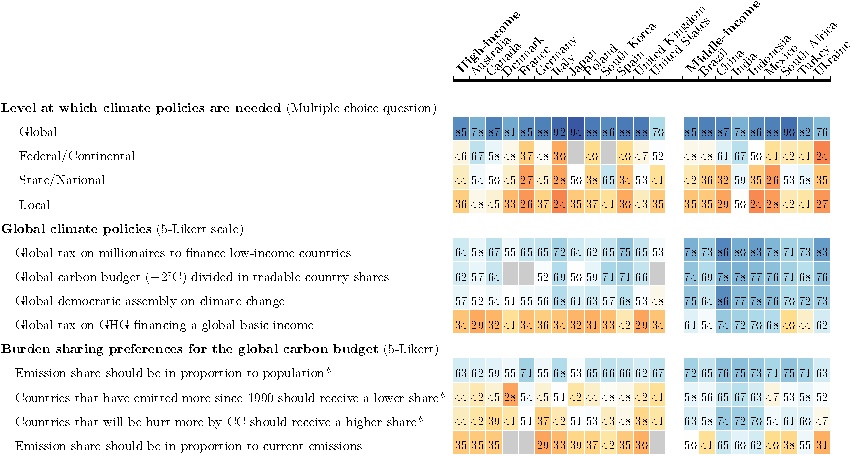
\includegraphics[width=1.2\textwidth]{../figures/OECD/Heatplot_global_tax_attitudes_positive.pdf}}\label{fig:oecd_absolute}% with dependence on others (absent from OECD): Heatplot_burden_share_all_positive_countries
    {\footnotesize \\ *In Denmark, France and the U.S., the questions with an asterisk were asked differently, cf. Question \ref{q:burden_sharing_asterisk}. } 
\end{figure}

\begin{figure}[h!]
    \caption[Comprehension]{Correct answers to comprehension questions (in percent). (Questions \ref{q:understood_gcs}-\ref{q:understood_both})}\label{fig:understood_each}
    \makebox[\textwidth][c]{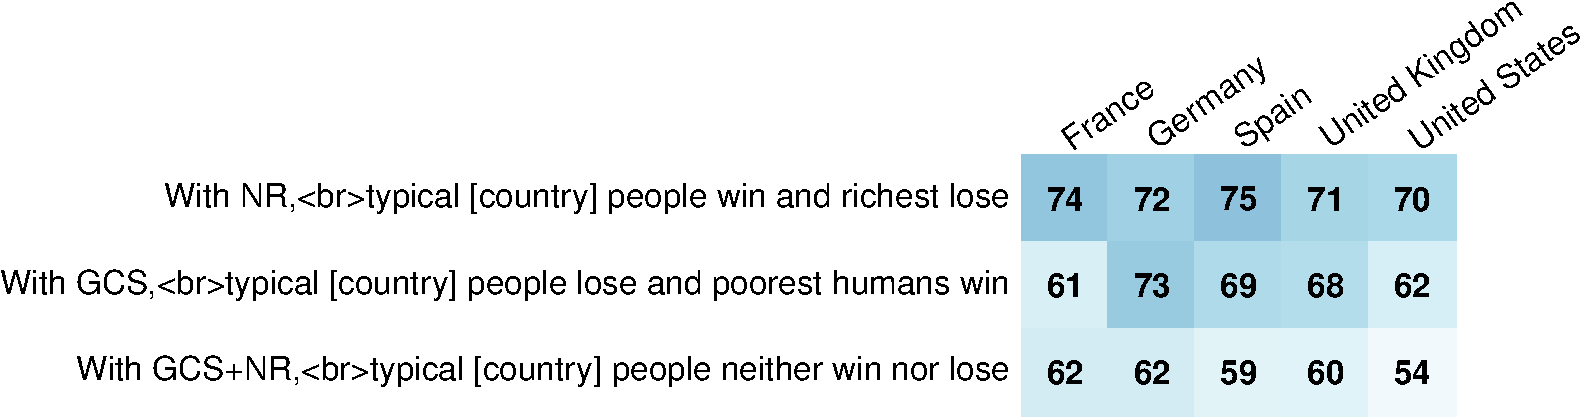
\includegraphics[width=\textwidth]{../figures/country_comparison/understood_each_positive.pdf}} 
\end{figure}

\begin{figure}[h!]
    \caption[Comprehension score]{Number of correct answers to comprehension questions (mean). (Section \ref{subsubsec:support_gcs}, Questions \ref{q:understood_gcs}-\ref{q:understood_both})}\label{fig:understood_score}
    \makebox[\textwidth][c]{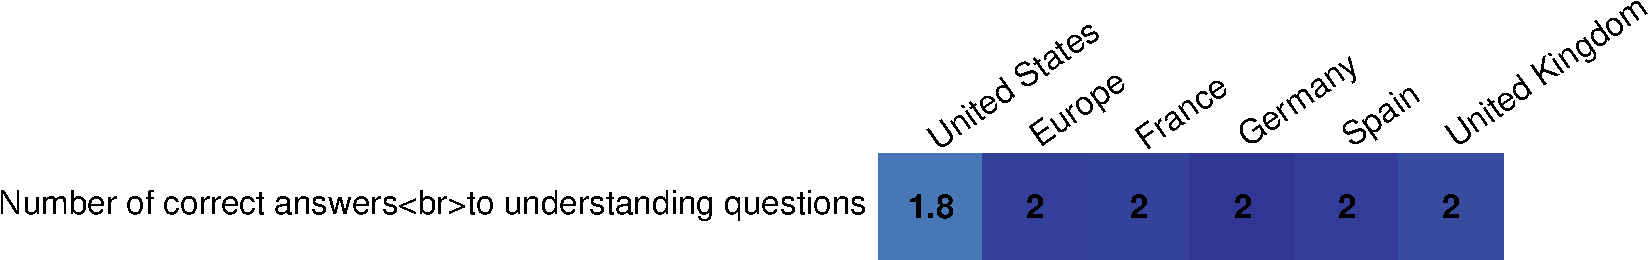
\includegraphics[width=\textwidth]{../figures/country_comparison/understood_score_mean.pdf}} 
\end{figure}

% \begin{figure}[h!]
%     \caption[Support for the Global Climate Scheme]{Support for the GCS, NR and the combination of GCS, NR and C. (Questions \ref{q:gcs_support}, \ref{q:nr_support} and \ref{q:crg_support})}\label{fig:support_binary}
%     \makebox[\textwidth][c]{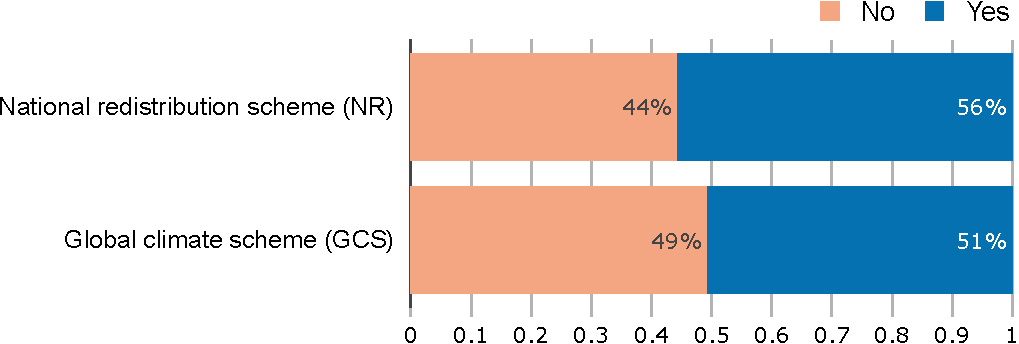
\includegraphics[width=.9\textwidth]{../figures/country_comparison/support_binary.pdf}} 
% \end{figure}

% \begin{figure}[h!]
%     \caption[Beliefs about support for the GCS and NR]{Beliefs regarding the support for the GCS and NR. (Questions \ref{q:gcs_belief} and \ref{q:nr_belief})}\label{fig:belief}
%     \makebox[\textwidth][c]{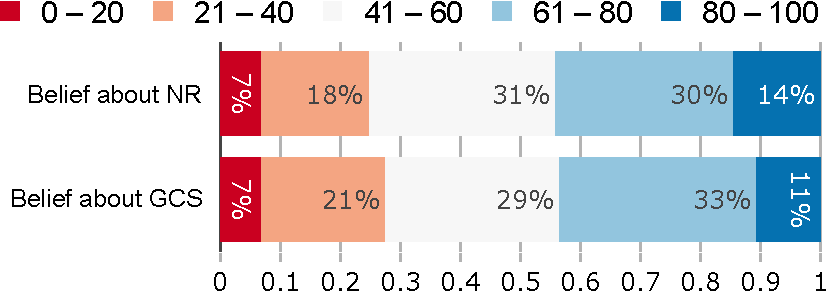
\includegraphics[width=.8\textwidth]{../figures/country_comparison/belief.pdf}} 
% \end{figure}

\begin{figure}[h!]
    \caption[List experiment]{List experiment: mean number of supported policies. (Section \ref{subsubsec:list_exp}, Question \ref{q:list_exp})}\label{fig:list_exp}
    \makebox[\textwidth][c]{
\includegraphics[width=.7\textwidth]{../figures/country_comparison/list_exp_mean.pdf}} 
\end{figure}

\begin{figure}[h!]
    \caption[Conjoint analyses 1 and 2]{Conjoint analyses 1 and 2. (Questions \ref{q:conjoint_a}-\ref{q:conjoint_b}, Back to Section \ref{subsubsec:conjoint})}\label{fig:conjoint}
    \makebox[\textwidth][c]{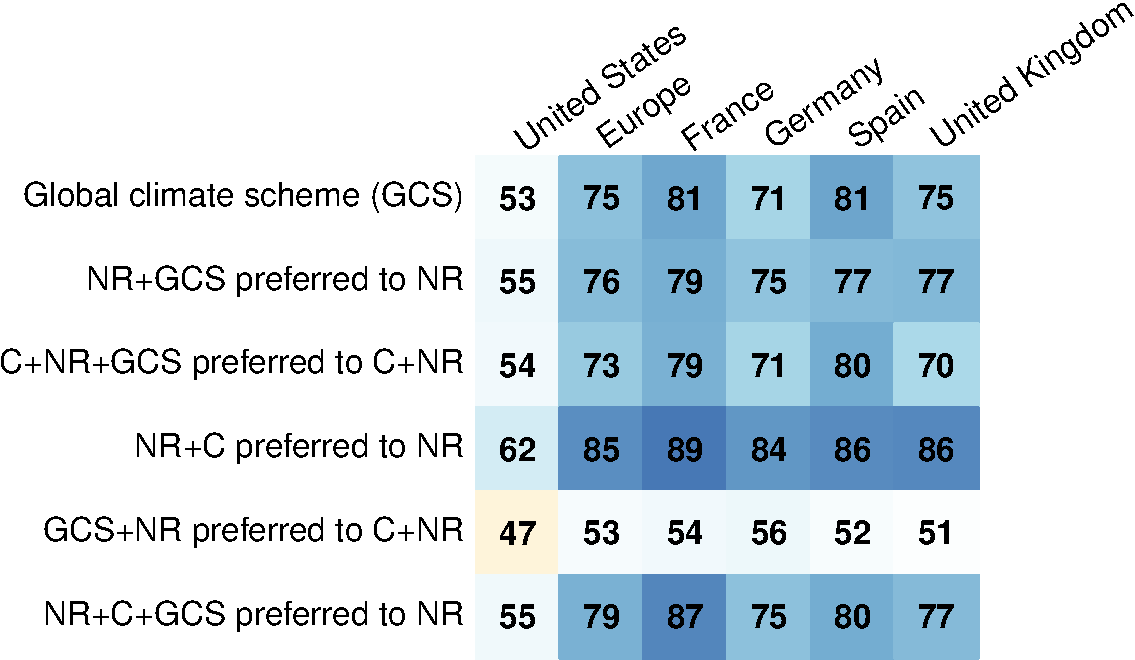
\includegraphics[width=.8\textwidth]{../figures/country_comparison/conjoint_ab_all_positive.pdf}} 
\end{figure}

% \begin{figure}[h!] % already in text
%     \caption{[Asked only to non-Republicans] Conjoint analysis n°4: random programs at the Democratic primary. (Question \ref{q:conjoint_r})}\label{fig:ca_r}
%     \makebox[\textwidth][c]{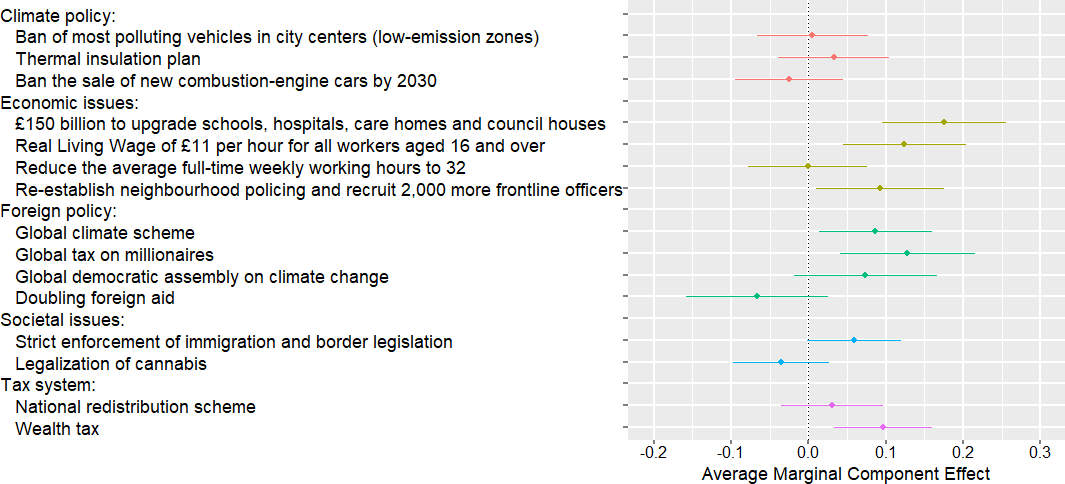
\includegraphics[width=\textwidth]{../figures/country_comparison/ca_r.png}} 
% \end{figure}

% \begin{figure}[h!]
%     \caption[Influence of the GCS on preferred platform]{Influence of the GCS on preferred platform:\\ Preference for a random platform A that contains the Global Climate Scheme rather than a platform B that does not (in percent). (Question \ref{q:conjoint_d}; in the U.S., asked only to non-Republicans.)}\label{fig:conjoint_left_ag_b}
%     \makebox[\textwidth][c]{
\includegraphics[width=\textwidth]{../figures/country_comparison/conjoint_left_ag_b_binary_positive.pdf}} 
% \end{figure}

\begin{figure}[h] 
  \caption[Preferences for various policies in political platforms (English)]{Effects of the presence of a policy (rather than none from this domain) in a random platform on the likelihood that it is preferred to another random platform. (See original translations in Figure \ref{fig:ca_r}; Question \ref{q:conjoint_r}%; in the U.S., asked only to non-Republicans.
  )}\label{fig:ca_r_en}
    \begin{subfigure}{.97\textwidth}
      \subcaption{Germany}
      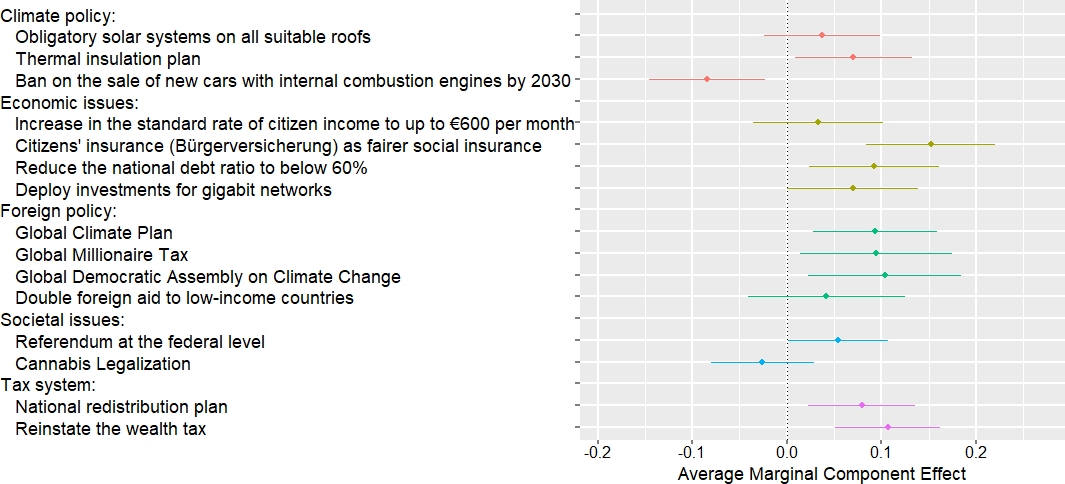
\includegraphics[width=.97\textwidth]{../figures/DE/ca_r_en.png}
    \end{subfigure}
    \begin{subfigure}{.98\textwidth}
      \subcaption{France}
      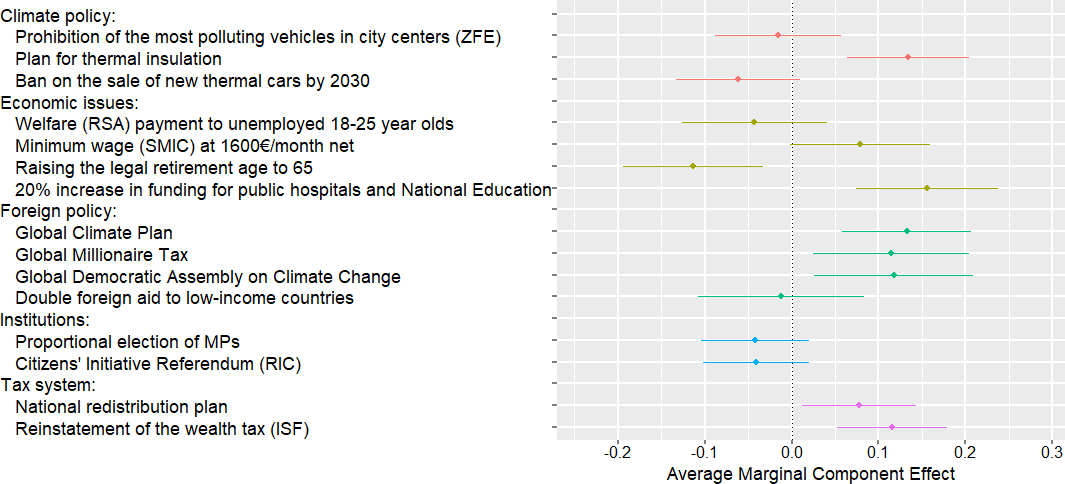
\includegraphics[width=.98\textwidth]{../figures/FR/ca_r_en.png}
    \end{subfigure}
    \begin{subfigure}{.98\textwidth}
      \subcaption{Spain}
      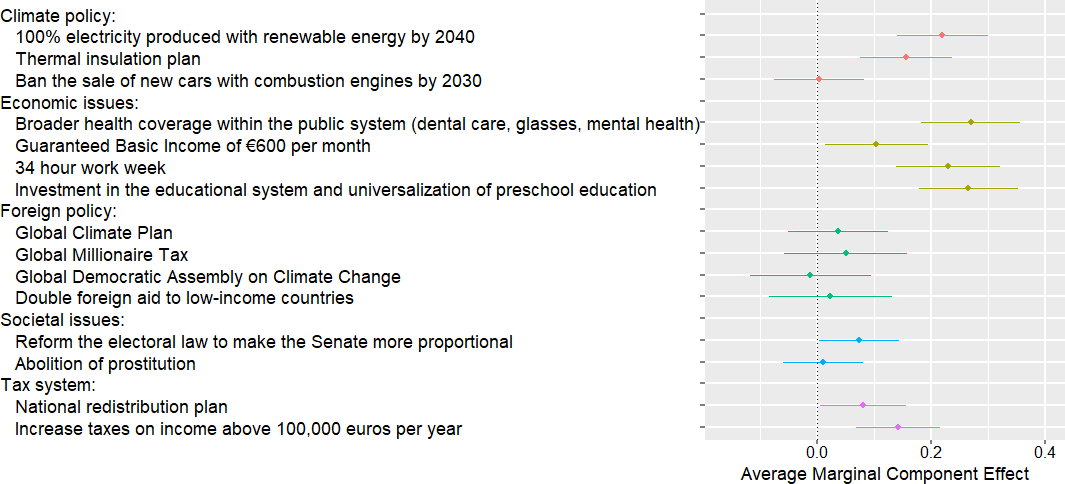
\includegraphics[width=.98\textwidth]{../figures/ES/ca_r_en.png}
    \end{subfigure}
\end{figure}

\begin{figure}[h!]
    \caption[Perceptions of the GCS]{Perceptions of the GCS. Elements seen as important for supporting the GCS in a 4-Likert scale (in percent). (Question \ref{q:gcs_important})  \hfill (Back~to~Section~\ref{subsubsec:pros_cons})}\label{fig:gcs_important}
    \makebox[\textwidth][c]{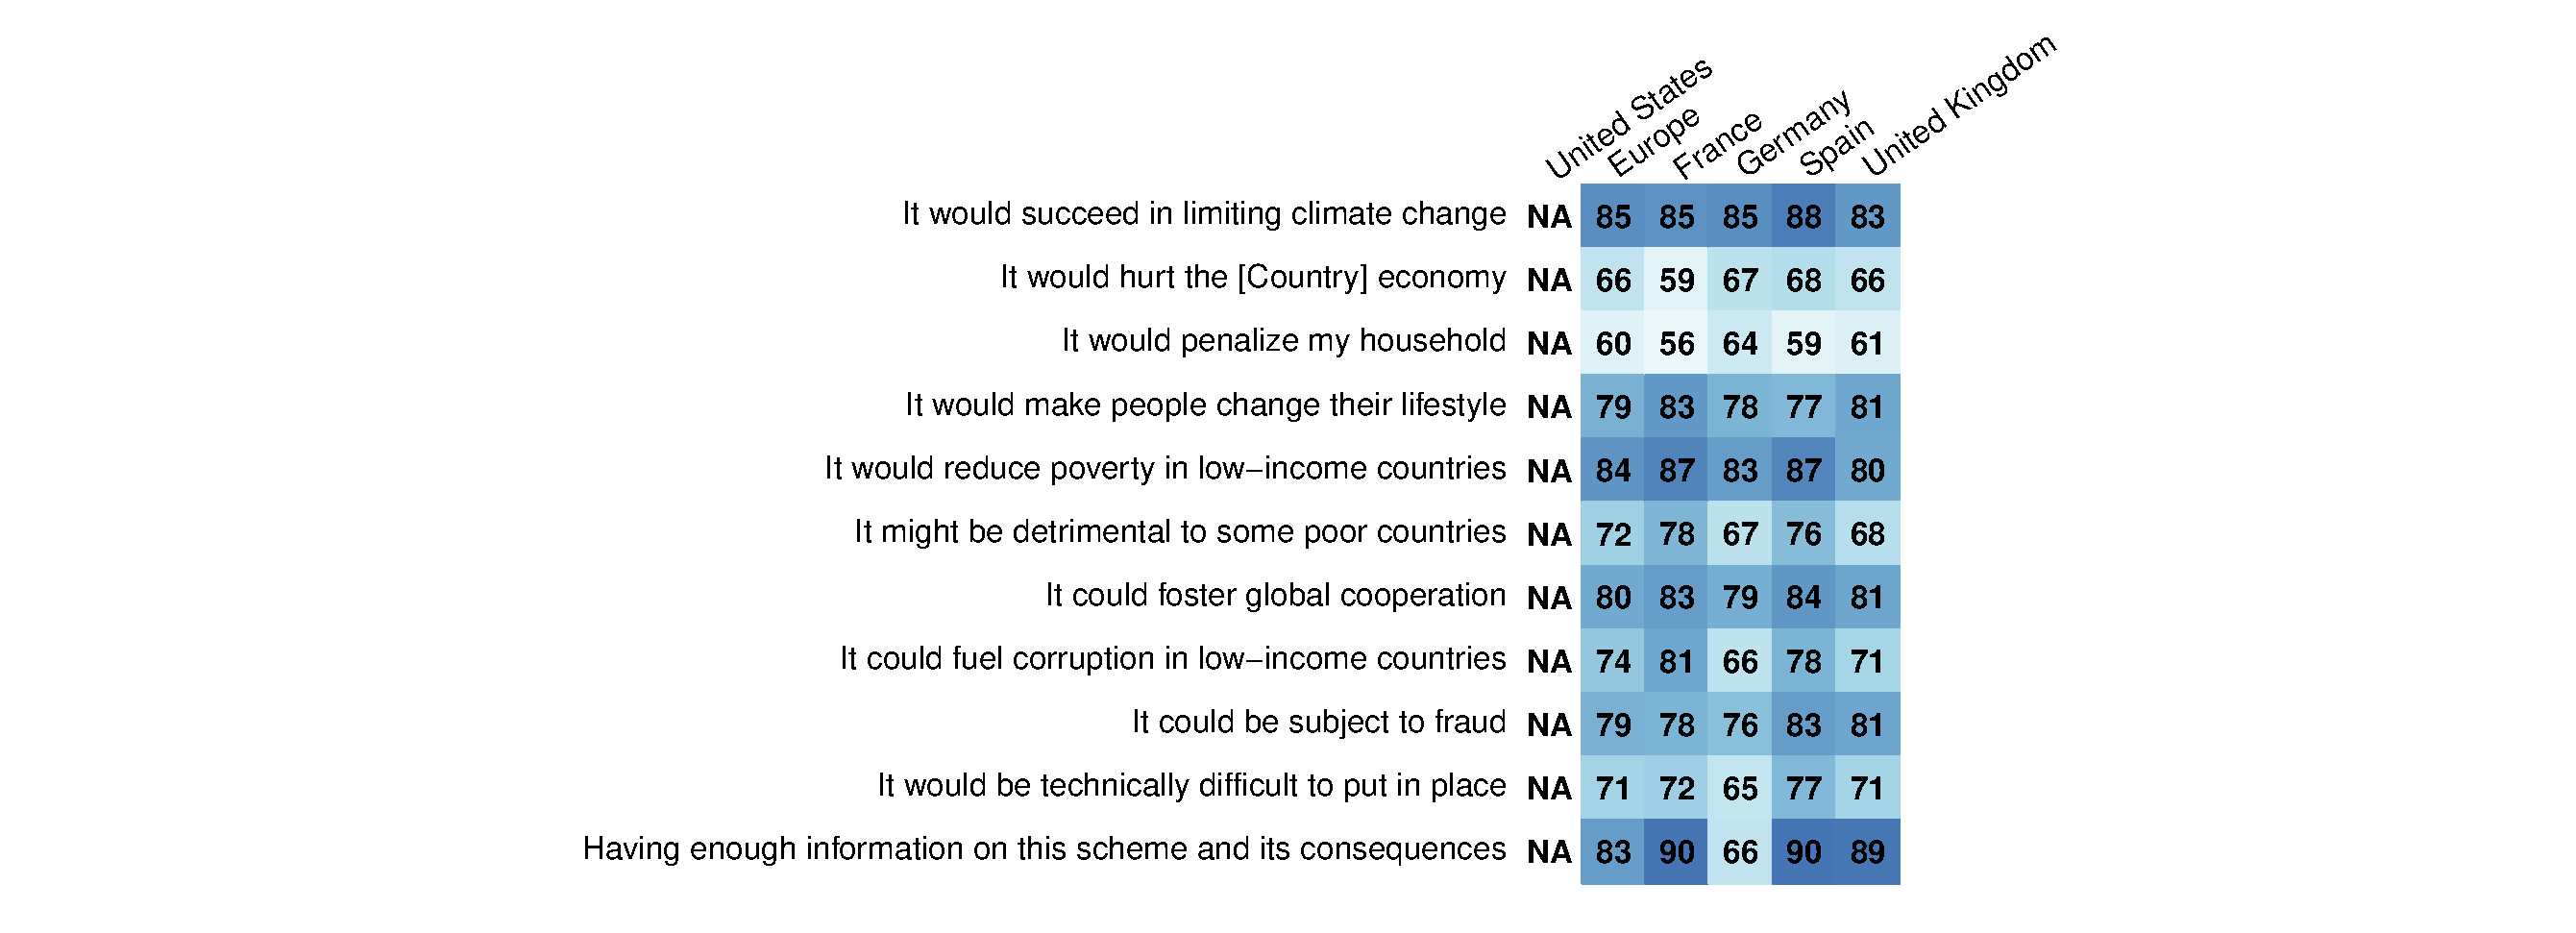
\includegraphics[width=\textwidth]{../figures/country_comparison/gcs_important_positive.pdf}} 
\end{figure}

\begin{figure}[h!]
    \caption[Classification of open-ended field on the GCS]{Perceptions of the GCS. Elements found in the open-ended field on the GCS (manually recoded, in percent). (Question \ref{q:gcs_field}) \hfill (Back~to~Section~\ref{subsubsec:pros_cons})}\label{fig:gcs_field}
    \makebox[\textwidth][c]{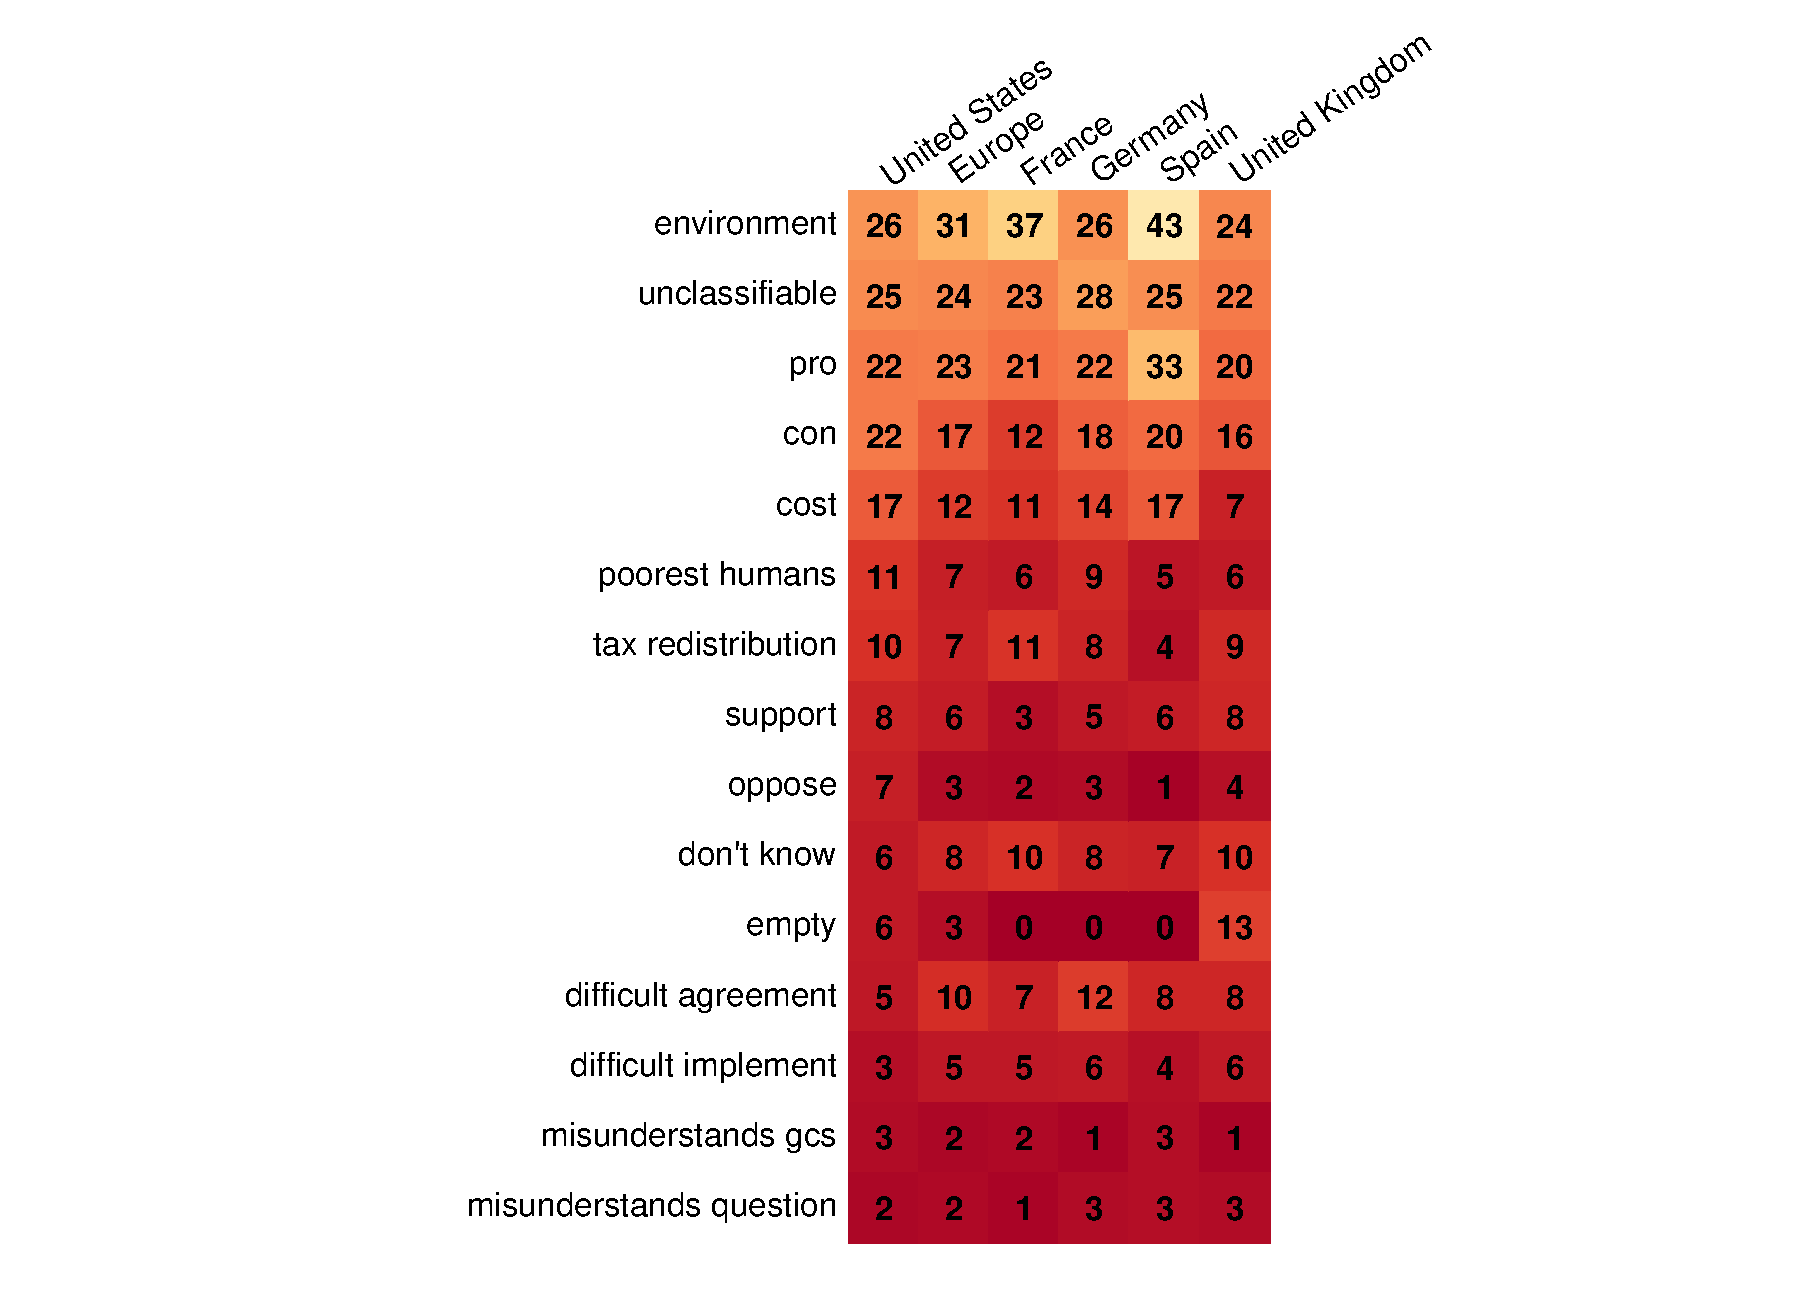
\includegraphics[width=.75\textwidth]{../figures/country_comparison/gcs_field_positive.pdf}} 
\end{figure}

\begin{figure}[h!]
    \caption[Topics of open-ended field on the GCS]{Perceptions of the GCS. Keywords found in the open-ended field on the GCS (automatic search ignoring case, in percent). (Question \ref{q:gcs_field}) \hfill (Back~to~Section~\ref{subsubsec:pros_cons})}\label{fig:gcs_field_contains}
    \makebox[\textwidth][c]{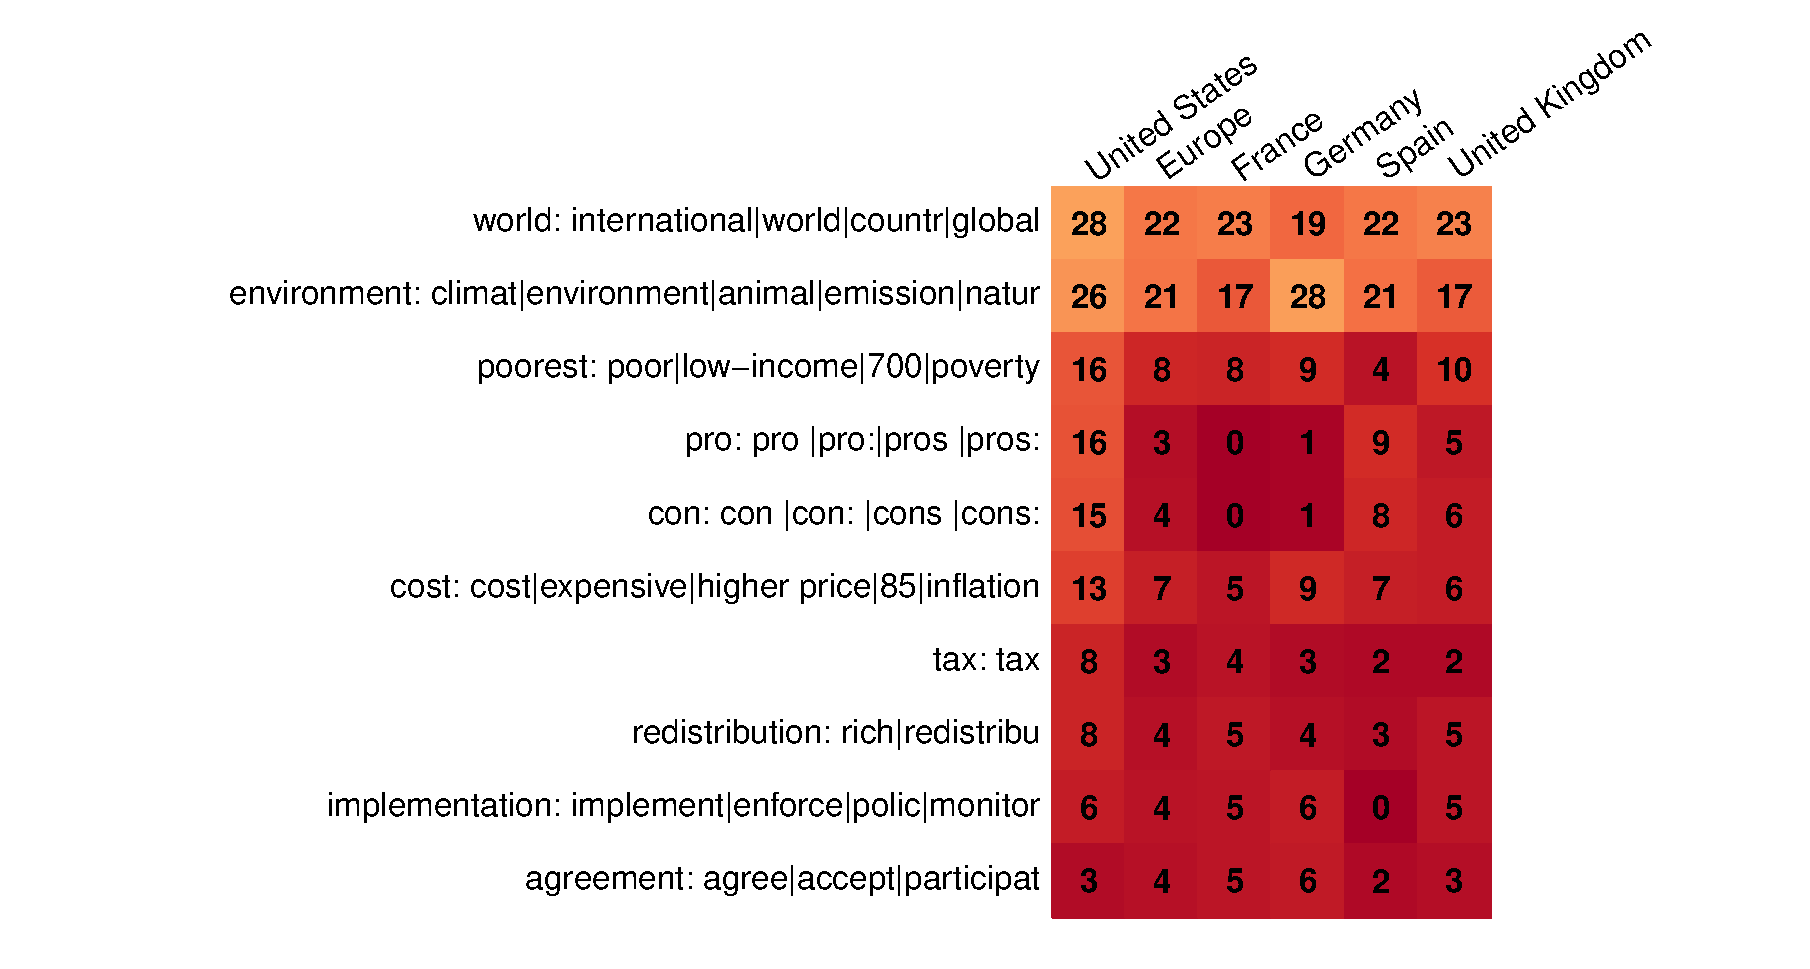
\includegraphics[width=\textwidth]{../figures/country_comparison/gcs_field_contains_positive.pdf}} 
\end{figure}

\begin{table}[h]
    \caption[Campaign and bandwagon effects on the support for the GCS.]{Effects on the support for the GCS of a question on its pros and cons and on information about the actual support, in the U.S. (See Section \ref{subsec:questionnaire_perceptions} in the US2 Questionnaire)  \hfill (Back~to~Section~\ref{subsubsec:pros_cons})} \label{tab:branch_gcs}
    \makebox[\textwidth][c]{
        
\begin{tabular}{@{\extracolsep{5pt}}lcccc} 
\\[-1.8ex]\hline 
\hline \\[-1.8ex] 
 & \multicolumn{4}{c}{Support} \\ 
\cline{2-5} 
\\[-1.8ex] & \multicolumn{2}{c}{Global Climate Scheme} & \multicolumn{2}{c}{National Redistribution} \\ 
\\[-1.8ex] & (1) & (2) & (3) & (4)\\ 
\hline \\[-1.8ex] 
Control group mean & 0.557 & 0.557 & 0.569 & 0.569  \\ \hline \\[-1.8ex]
 Treatment: Open\mbox{-}ended field on GCS pros \& cons & $-$0.073$^{**}$ & $-$0.071$^{**}$ & $-$0.035 & $-$0.030 \\ 
  & (0.035) & (0.031) & (0.035) & (0.032) \\ 
  Treatment: Closed questions on GCS pros \& cons & $-$0.109$^{***}$ & $-$0.096$^{***}$ & $-$0.065$^{*}$ & $-$0.062$^{**}$ \\ 
  & (0.034) & (0.031) & (0.034) & (0.031) \\ 
  Treatment: Info on actual support for GCS and NR & $-$0.021 & $-$0.015 & 0.048 & 0.056$^{*}$ \\ 
  & (0.034) & (0.031) & (0.033) & (0.031) \\ 
 \hline \\[-1.8ex] 
Includes controls &  & \checkmark &  & \checkmark \\

Observations & 2,000 & 1,995 & 2,000 & 1,995 \\ 
R$^{2}$ & 0.007 & 0.170 & 0.007 & 0.154 \\ 
\hline 
\hline \\[-1.8ex] 
\end{tabular} 
    }
    {\footnotesize %\textit{Note}: 
    }
\end{table}

\begin{figure}[h!]
    \caption[Donation to Africa vs. own country]{Donation in case of lottery win, depending on the recipient's (randomly drawn) nationality (mean). (Question \ref{q:donation})\hfill (Back~to~Section~\ref{subsec:universalistic})}\label{fig:donation}
    \makebox[\textwidth][c]{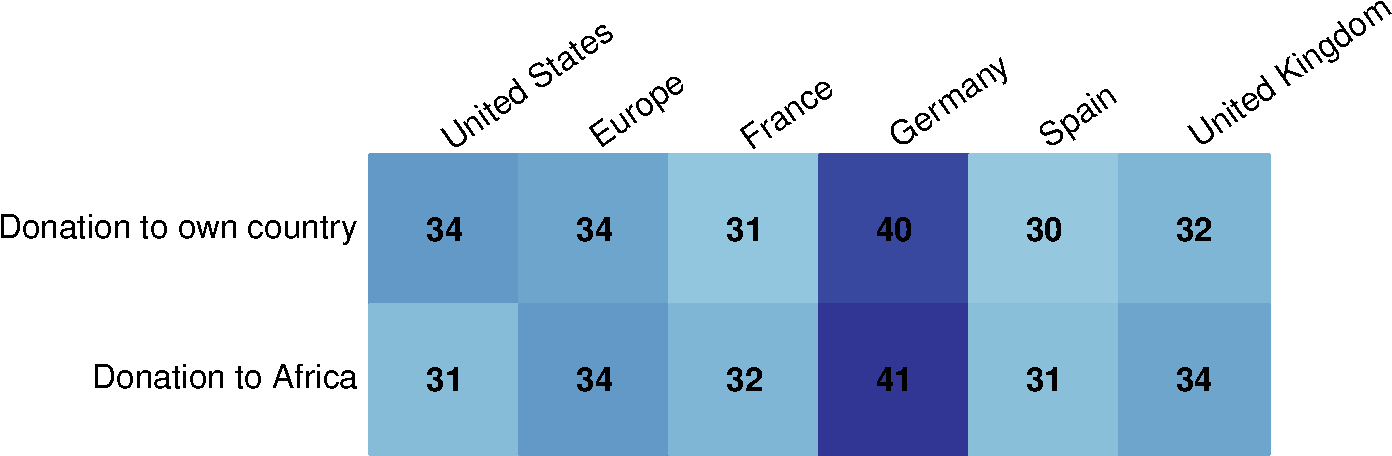
\includegraphics[width=.8\textwidth]{../figures/country_comparison/donation_mean.pdf}} 
\end{figure}

\begin{table}[h]
    \caption[Donation to Africa vs. own country]{Donation in case of lottery win, depending on the recipient's (randomly drawn) nationality. (Question \ref{q:donation})\hfill (Back~to~Section~\ref{subsec:universalistic})} \label{tab:donation}
    \makebox[\textwidth][c]{
\begin{tabular}{@{\extracolsep{5pt}}lcccc} 
\\[-1.8ex]\hline 
\hline \\[-1.8ex] 
 & \multicolumn{4}{c}{Donation to poor people (in \%)} \\ 
\cline{2-5} 
\\[-1.8ex] & All & US & US & Eu \\ 
\hline \\[-1.8ex] 
 Poor is in own country & 0.590 & 2.509$^{**}$ & 0.046 & $-$1.349 \\ 
  & (0.799) & (1.152) & (1.691) & (1.108) \\ 
  Poor is in own country $\times$ Vote: \textit{not} Biden &  &  & 3.954$^{*}$ &  \\ 
  &  &  & (2.279) &  \\ 
 \hline \\[-1.8ex] 
Mean & 34.034 & 33.658 & 33.658 & 34.41 \\ 
Observations & 6,000 & 3,000 & 3,000 & 3,000 \\ 
R$^{2}$ & 0.0001 & 0.002 & 0.034 & 0.0005 \\ 
\hline 
\hline \\[-1.8ex] 
\end{tabular} }
\end{table}

\begin{figure}[h!]
    \caption[Support for a global wealth tax]{Support for a global wealth tax. \\
    ``Do you support or oppose a tax on millionaires of all countries to finance low-
    income countries? \\
    Such tax would finance infrastructure and public services such as access to drinking water, healthcare, and education.'' (Question \ref{q:global_tax})}\label{fig:global_tax}
    \makebox[\textwidth][c]{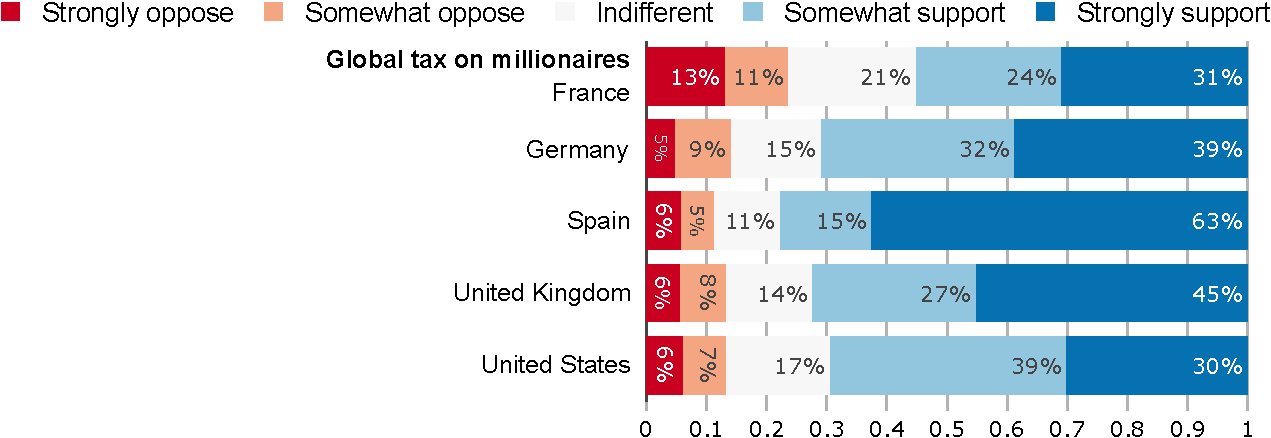
\includegraphics[width=\textwidth]{../figures/country_comparison/global_tax_support.pdf}} 
\end{figure}

\begin{figure}[h!]
    \caption[Support for a national wealth tax]{Support for a national wealth tax financing public services like healthcare, education, and social housing. (Question \ref{q:national_tax})}\label{fig:national_tax}
    \makebox[\textwidth][c]{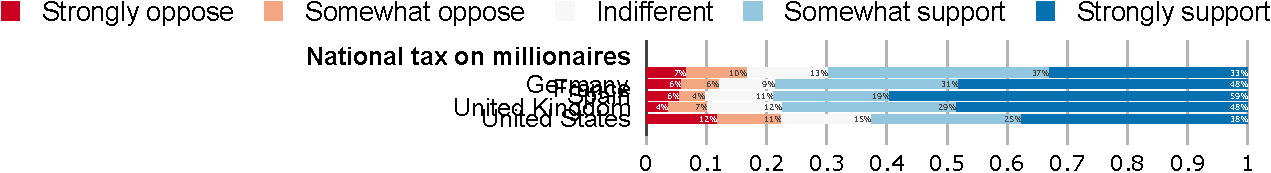
\includegraphics[width=\textwidth]{../figures/country_comparison/national_tax_support.pdf}} 
\end{figure}

\begin{figure}[h!]
    \caption[Preferred share of global tax for low-income countries]{Preferred share of global wealth tax revenues that should be pooled to finance low-income countries. (Question \ref{q:global_tax_global_share})}\label{fig:global_tax_global_share}
    \makebox[\textwidth][c]{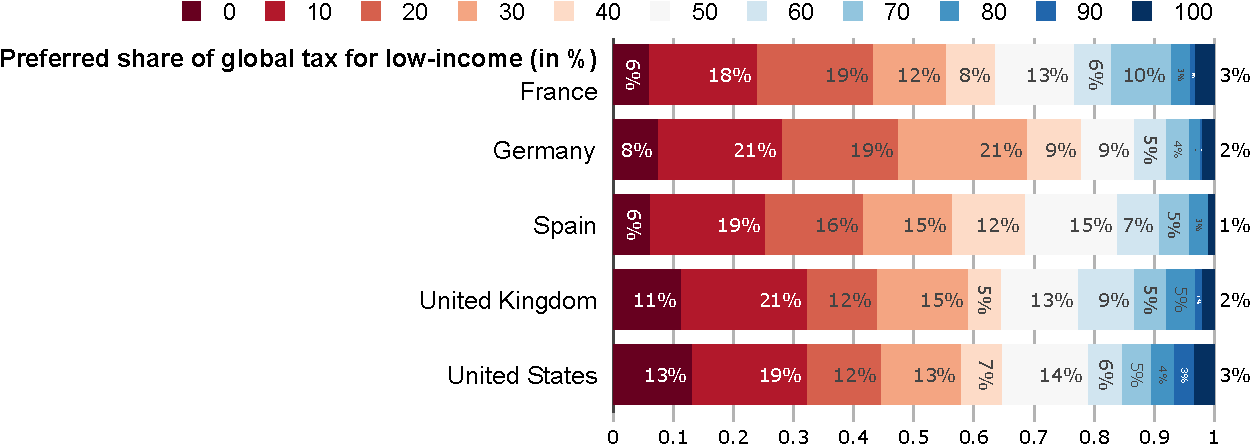
\includegraphics[width=\textwidth]{../figures/country_comparison/global_tax_global_share.pdf}} 
\end{figure}

\begin{figure}[h!]
    \caption[Support for sharing half of global tax revenues with low-income countries]{Support for sharing half of global tax revenues with low-income countries, rather that each country retaining all the revenues it collects (in percent). (Question \ref{q:global_tax_sharing})}\label{fig:global_tax_sharing}
    \makebox[\textwidth][c]{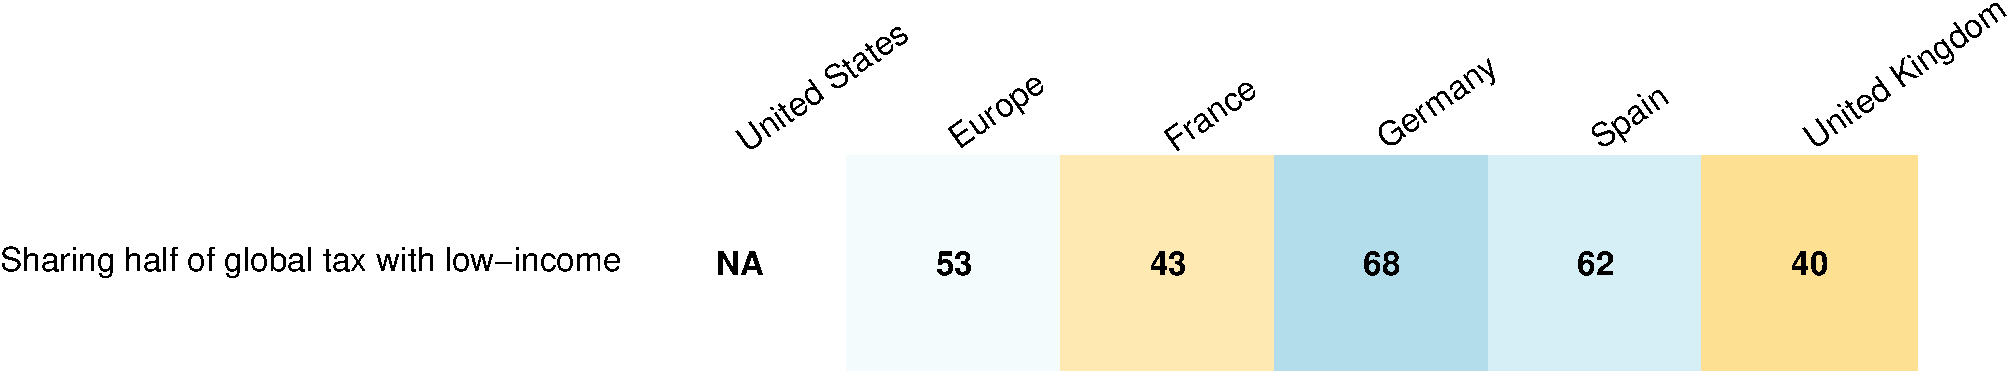
\includegraphics[width=\textwidth]{../figures/country_comparison/global_tax_sharing_positive.pdf}} 
\end{figure}

\begin{figure} 
    \caption[Actual, perceived and preferred amount of foreign aid (mean)]{Actual, perceived and preferred amount of foreign aid, with random info (or not) on actual amount. (\textit{Mean}, Questions \ref{q:foreign_aid_belief}, \ref{q:foreign_aid_preferred})  \hfill (Back~to~Section~\ref{subsubsec:support_foreign_aid})}\label{fig:foreign_aid_amount}
    \makebox[\textwidth][c]{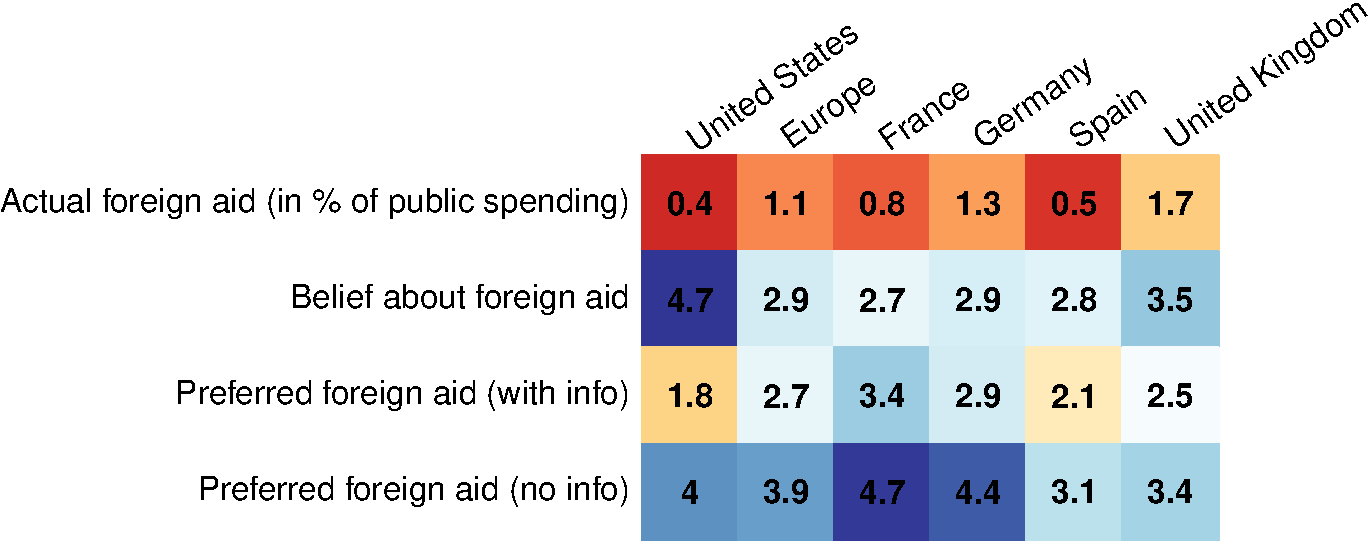
\includegraphics[width=.9\textwidth]{../figures/country_comparison/foreign_aid_amount_mean.pdf} } 
\end{figure}

% \begin{figure} 
%     \caption{Actual, perceived and preferred amount of foreign aid, with random info (or not) on actual amount. (\textit{Median}, Questions \ref{q:foreign_aid_belief}, \ref{q:foreign_aid_preferred})}\label{fig:foreign_aid_amount}
%     \makebox[\textwidth][c]{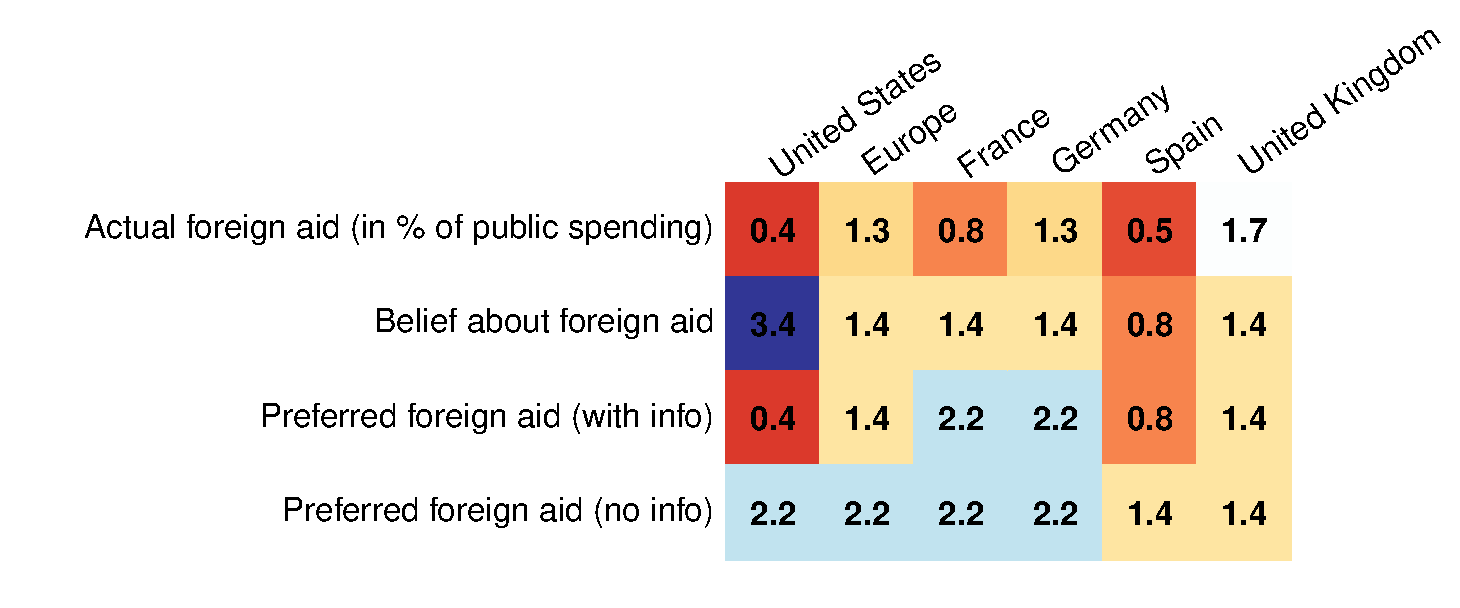
\includegraphics[width=.9\textwidth]{../figures/country_comparison/foreign_aid_amount_median.pdf} } % TODO? add? not necessary as the info on median can be deduced from below figures
% \end{figure}

\begin{figure} 
    % \caption{Support for increased foreign aid (vs. reduced or stable): from previous question, and directly asked (with info).}\vspace{-.2cm}
    % 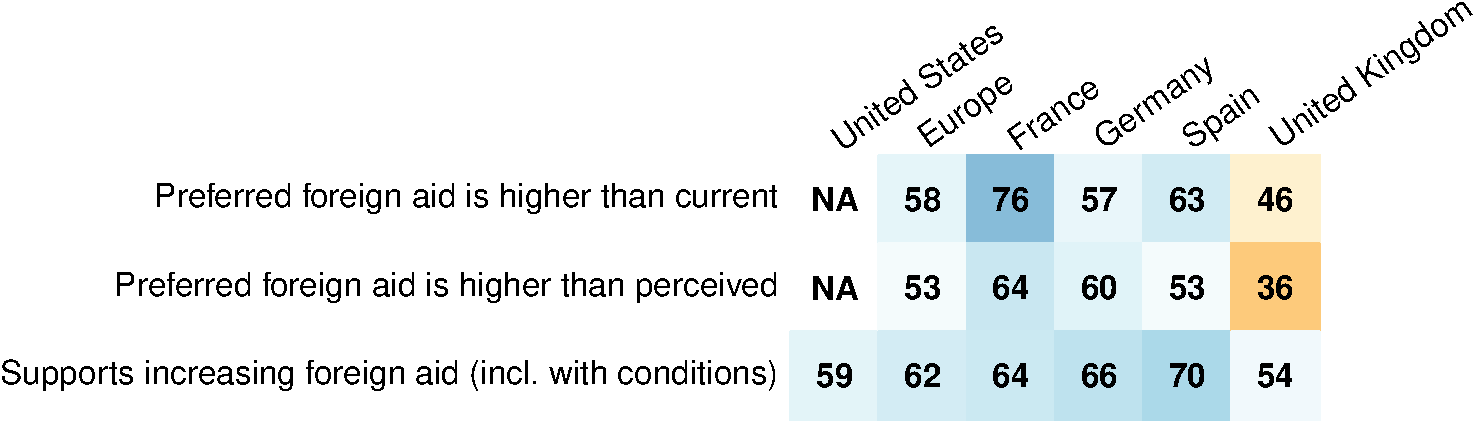
\includegraphics[height=.32\textheight]{../figures/country_comparison/foreign_aid_more_positive.pdf} 
    \caption[Preferred foreign aid (summary)]{Preferred foreign aid (after info or after perception). (Questions \ref{q:foreign_aid_belief} and \ref{q:foreign_aid_preferred})}\label{fig:foreign_aid_no_less_all}
    \makebox[\textwidth][c]{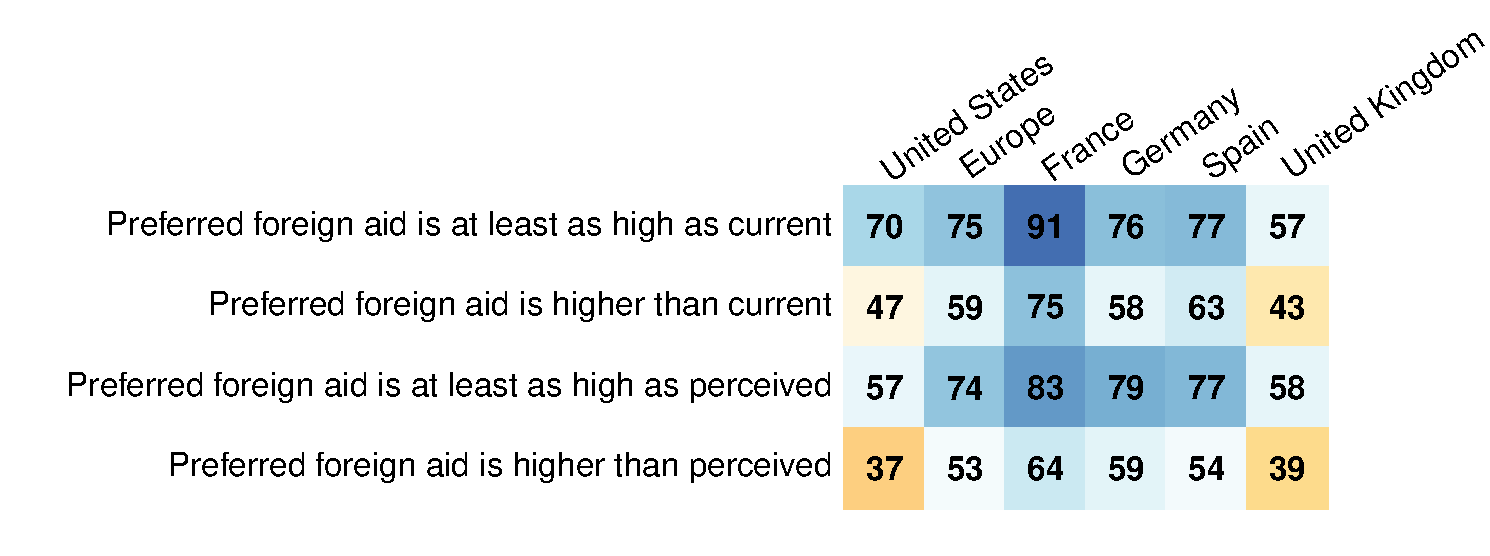
\includegraphics[width=\textwidth]{../figures/country_comparison/foreign_aid_no_less_all_positive.pdf} }
\end{figure} 

% \begin{figure}
%     \centering 
%     \caption{Your previous answer shows that you would like to increase [UK] foreign aid.\\How would you like to finance such increase in foreign aid? (Multiple answers possible)}
%     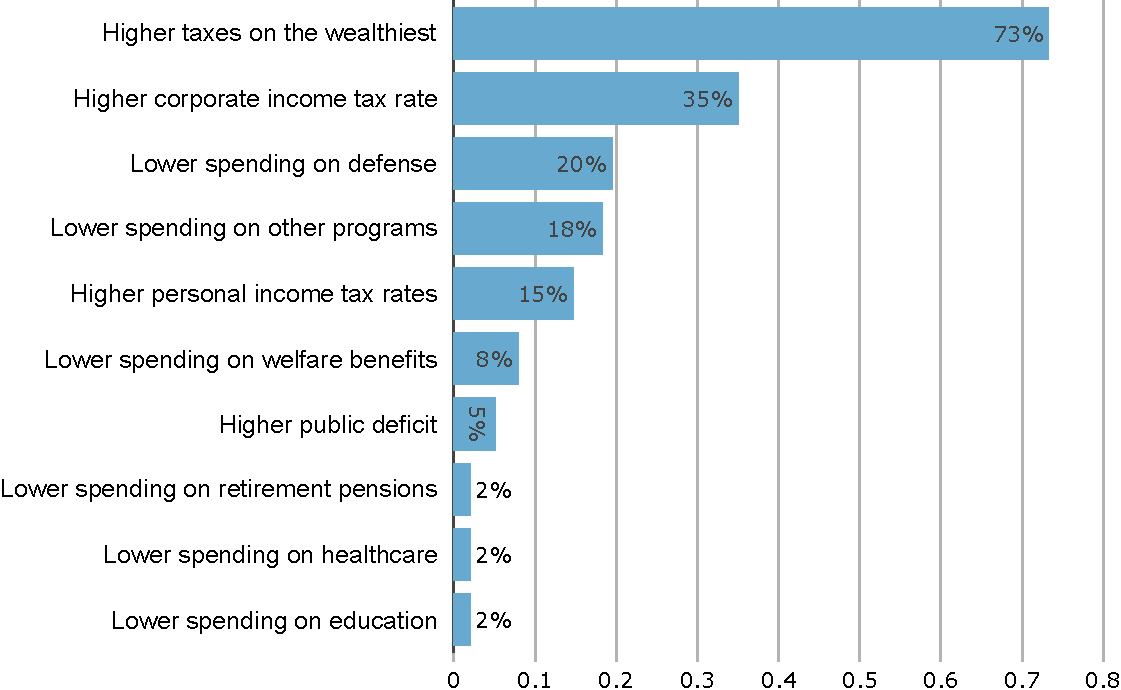
\includegraphics[width=\columnwidth]{../figures/all/foreign_aid_raise.pdf} 
% \end{figure}		
% \begin{figure}
%     \centering 
%     \caption{Your previous answer shows that you would like to reduce [UK] foreign aid.\\How would you like to use the freed budget? (Multiple answers possible)}
%     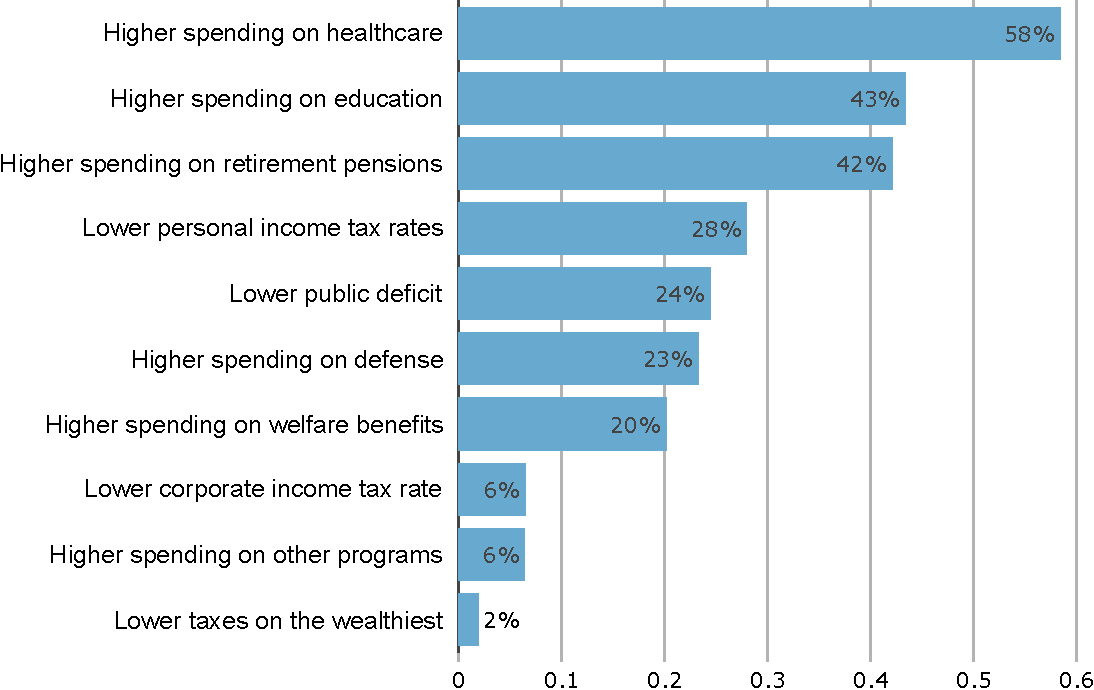
\includegraphics[width=\columnwidth]{../figures/all/foreign_aid_reduce.pdf} 
% \end{figure}

\begin{figure}[h!]
    \caption[Perceived foreign aid]{Perceived foreign aid. ``From your best guess, what percentage of [own country] government spending is allocated to foreign aid (that is, to reduce poverty in low-income countries)?'' (Question \ref{q:foreign_aid_belief})  \hfill (Back~to~Section~\ref{subsubsec:support_foreign_aid}) \\ Actual values: France: 0.8\%; Germany: 1.3\%; Spain: 0.5\%; UK: 1.7\%; U.S.: 0.4\%.}\label{fig:foreign_aid_belief}
    \makebox[\textwidth][c]{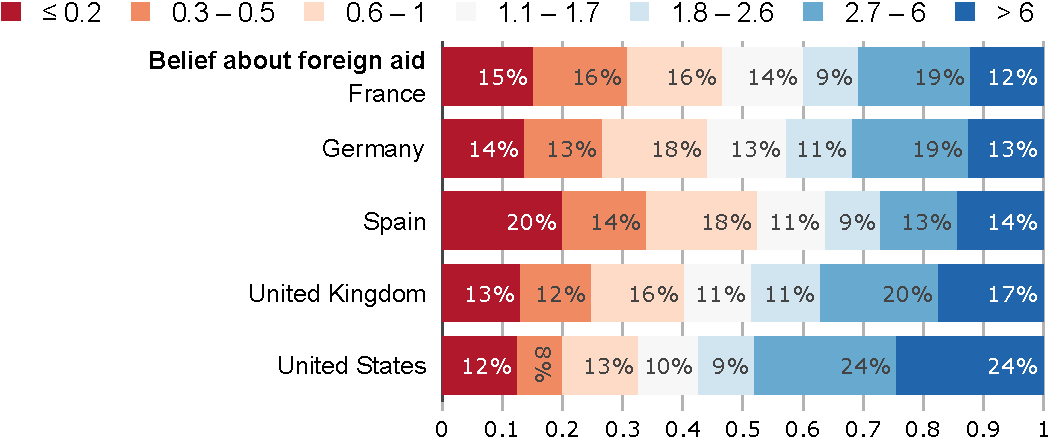
\includegraphics[width=\textwidth]{../figures/country_comparison/foreign_aid_belief_agg.pdf}} 
\end{figure}

\begin{figure}[h!]
    \caption[Preferred foreign aid (without info on actual amount)]{Preferred foreign aid (without info on actual amount). \\ ``If you could choose the government spending, what percentage would you allocate
    to foreign aid?'' (Question \ref{q:foreign_aid_preferred})  \hfill (Back~to~Section~\ref{subsubsec:support_foreign_aid})}\label{fig:foreign_aid_preferred_no_info}
    \makebox[\textwidth][c]{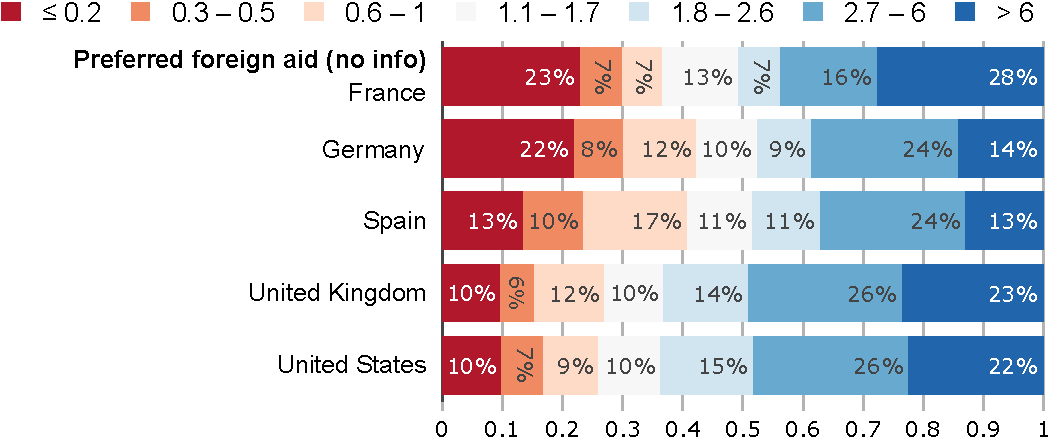
\includegraphics[width=\textwidth]{../figures/country_comparison/foreign_aid_preferred_no_info_agg.pdf}} 
\end{figure}

\begin{figure}[h!]
    \caption[Preferred foreign aid (after info on actual amount)]{Preferred foreign aid (after info on actual amount). \\ ``Actually,
    [US1: 0.4\%; FR: 0.8\%; DE: 1.3\%; ES: 0.5\%; UK: 1.7\%] of [own country] government spending is allocated to foreign aid. \\
    If you could choose the government spending, what percentage would you allocate
    to foreign aid?'' (Question \ref{q:foreign_aid_preferred})  \hfill (Back~to~Section~\ref{subsubsec:support_foreign_aid})}\label{fig:foreign_aid_preferred_info}
    \makebox[\textwidth][c]{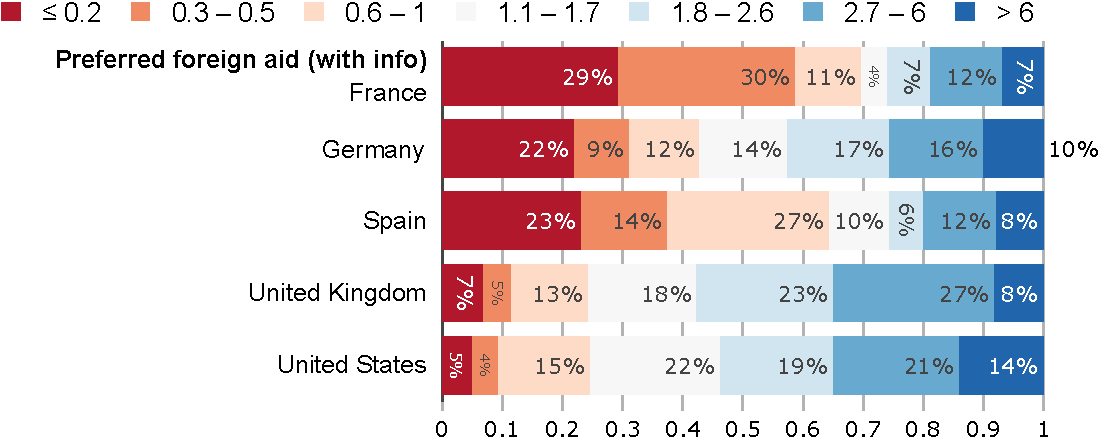
\includegraphics[width=\textwidth]{../figures/country_comparison/foreign_aid_preferred_info_agg.pdf}} 
\end{figure}

\begin{figure}[h!]
    \caption[Preferences for funding increased foreign aid]{Preferences for funding increased foreign aid. [Asked iff preferred foreign aid is strictly greater than [Info: actual; No info: perceived] foreign aid] \\ ``How would you like to finance such increase in foreign aid? (Multiple answers possible)'' (in percent) (Question \ref{q:foreign_aid_raise_how})  \hfill (Back~to~Section~\ref{subsubsec:support_foreign_aid})}\label{fig:foreign_aid_raise_how}
    \makebox[\textwidth][c]{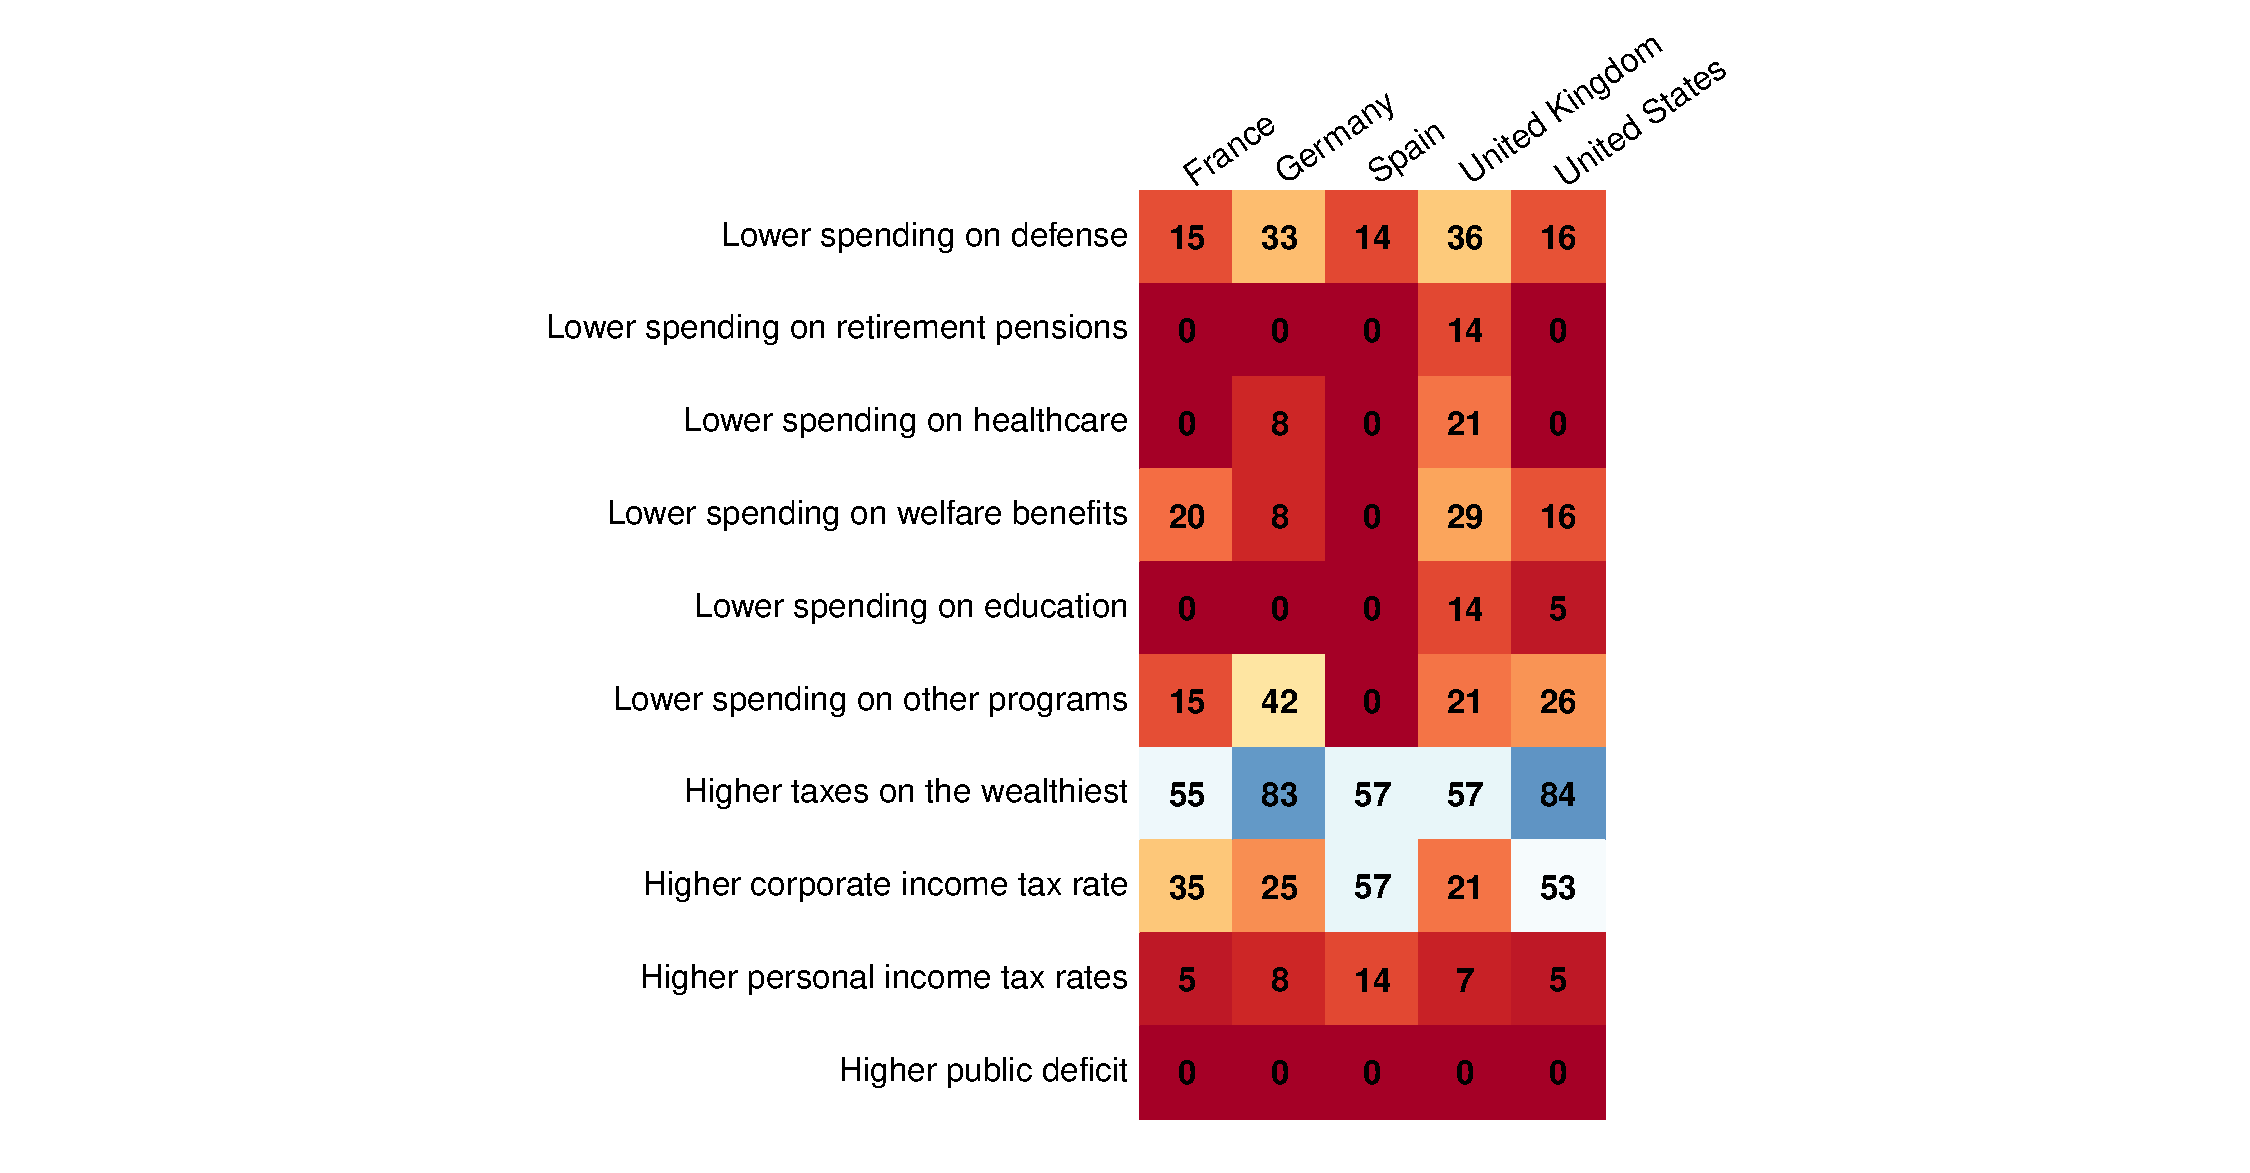
\includegraphics[width=.75\textwidth]{../figures/country_comparison/foreign_aid_raise_positive.pdf}} 
\end{figure}

\begin{figure}[h!]
    \caption[Preferences of spending following reduced foreign aid]{Preferences of spending following reduced foreign aid. [Asked iff preferred foreign aid is strictly lower than [Info: actual; No info: perceived] foreign aid] \\ ``How would you like to use the freed budget? (Multiple answers possible)'' (in percent) (Question \ref{q:foreign_aid_reduce_how})  \hfill (Back~to~Section~\ref{subsubsec:support_foreign_aid})}\label{fig:foreign_aid_reduce_how}
    \makebox[\textwidth][c]{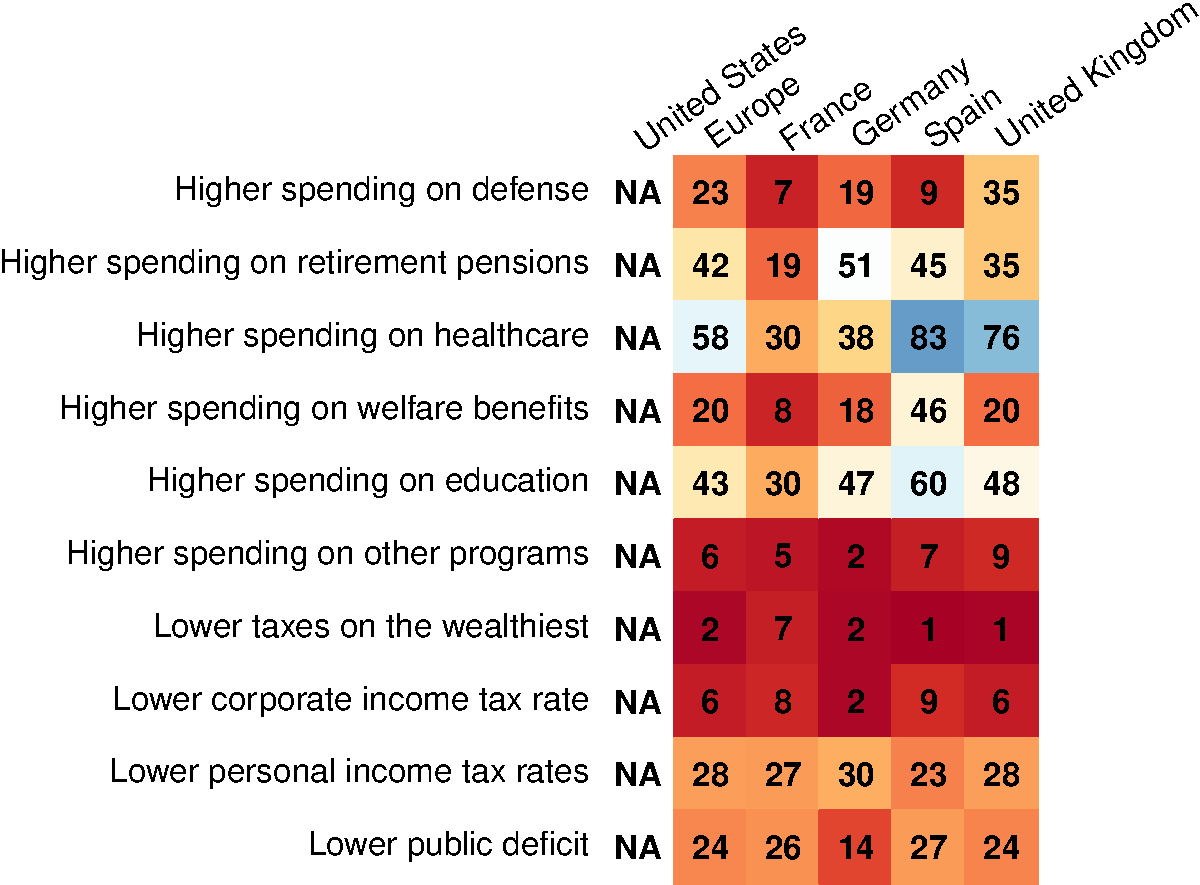
\includegraphics[width=.75\textwidth]{../figures/country_comparison/foreign_aid_reduce_positive.pdf}} 
\end{figure}

% \begin{figure}[h!]
%     \caption[Attitudes on the evolution of foreign aid]{Attitudes regarding the evolution of [own country] foreign aid. (Question \ref{q:foreign_aid_raise_support})}\label{fig:foreign_aid_raise_support}
%     \makebox[\textwidth][c]{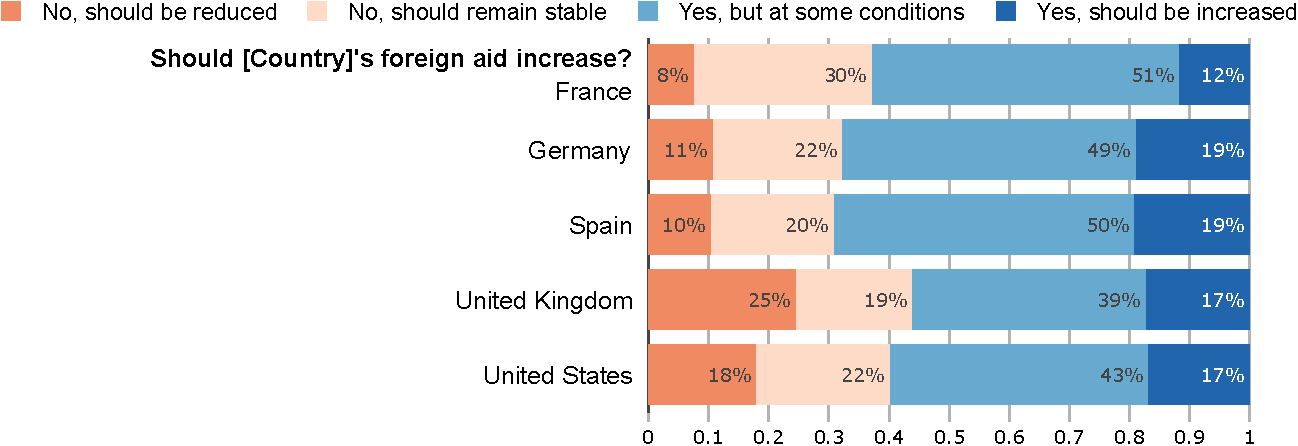
\includegraphics[width=\textwidth]{../figures/country_comparison/foreign_aid_raise_support.pdf}} 
% \end{figure}

% \begin{figure}[h!]
%     \caption[Conditions at which foreign aid should be increased]{Conditions at which foreign aid should be increased (in percent). [Asked to those who wish an increase of foreign aid at some conditions.] (Question \ref{q:foreign_aid_condition})}\label{fig:foreign_aid_condition}
%     \makebox[\textwidth][c]{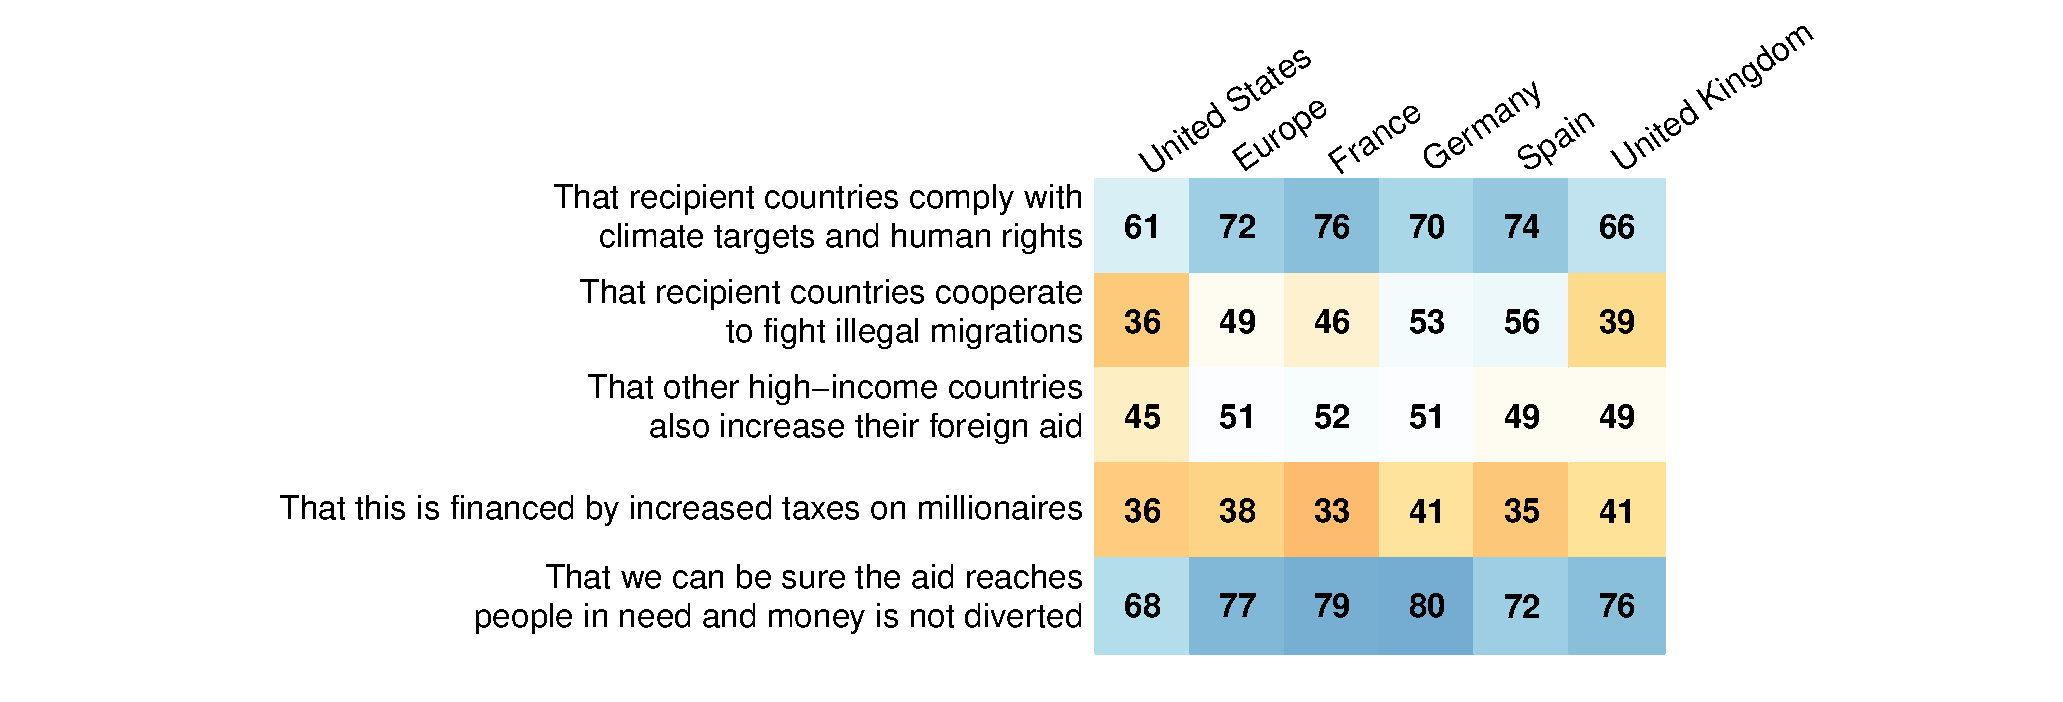
\includegraphics[width=\textwidth]{../figures/country_comparison/foreign_aid_condition_positive.pdf}} 
% \end{figure}

% \begin{figure}[h!]
%     \caption[Reasons why foreign aid should not be increased]{Reasons why foreign aid should not be increased (in percent). [Asked to those who wish a decrease or stability of foreign aid.] (Question \ref{q:foreign_aid_no})}\label{fig:foreign_aid_no}
%     \makebox[\textwidth][c]{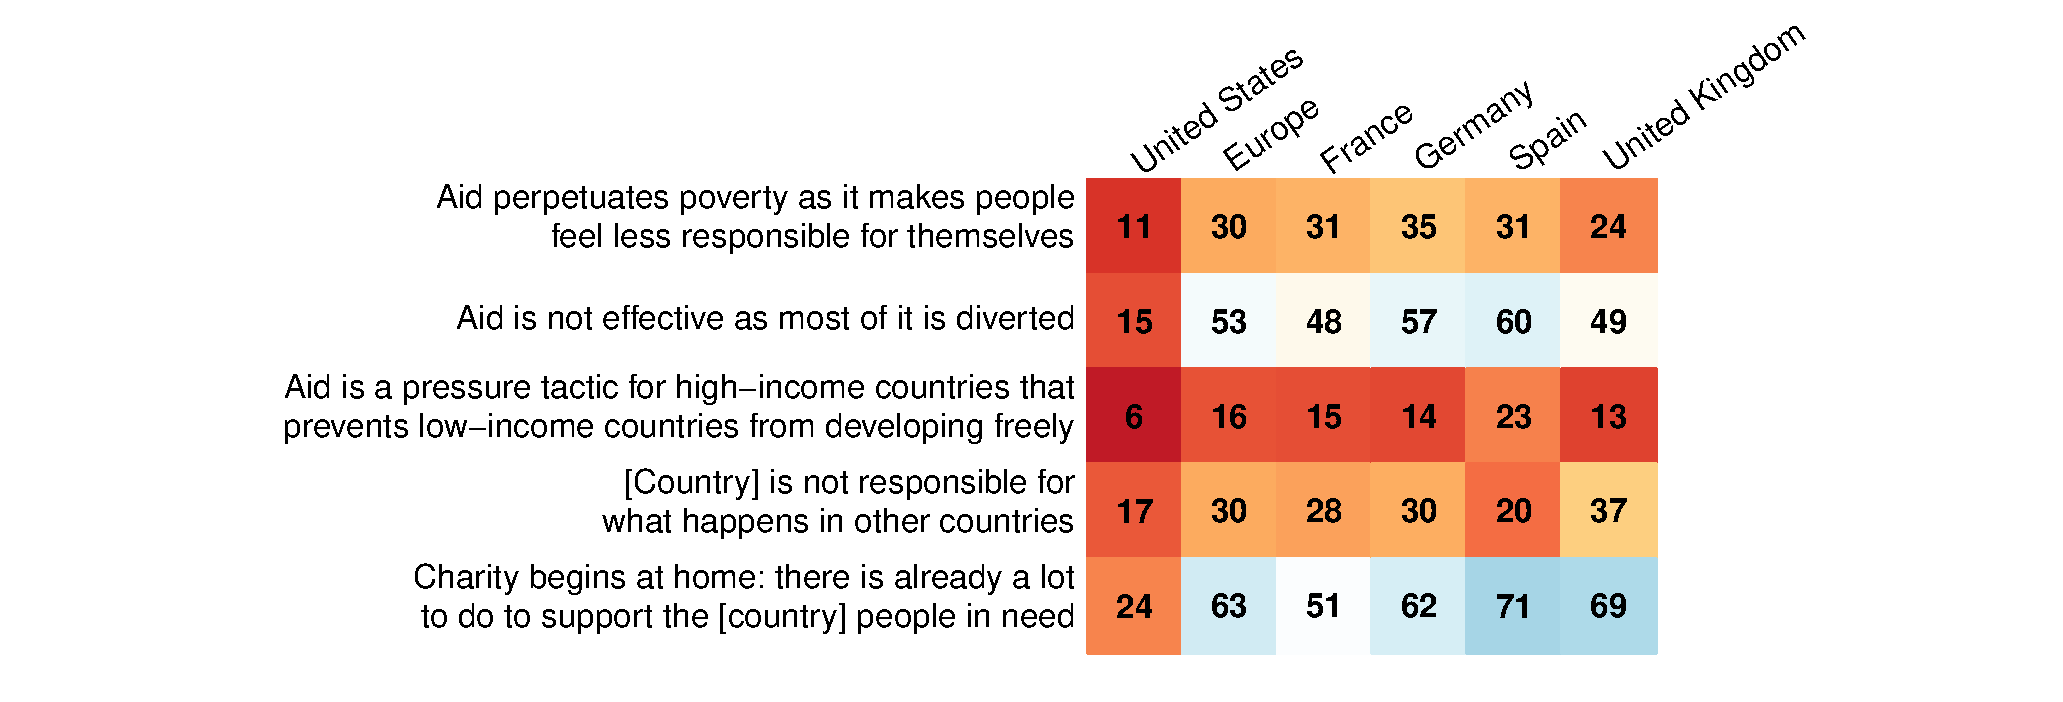
\includegraphics[width=\textwidth]{../figures/country_comparison/foreign_aid_no_positive.pdf}} 
% \end{figure}

% \begin{figure}[h!]
%     \caption[Willingness to sign a real-stake petition]{Willingness to sign real-stake petition for the Global Climate Scheme or National Redistribution. (Question \ref{q:petition})}\label{fig:petition}
%     \makebox[\textwidth][c]{
\includegraphics[width=.8\textwidth]{../figures/country_comparison/petition_only_positive.pdf}} 
% \end{figure}

\begin{figure}[h!]
    \caption[Willingness to sign a real-stake petition]{Willingness to sign real-stake petition for the Global Climate Scheme or National Redistribution, compared to stated support in corresponding subsamples (e.g. support for the GCS in the branch where the petition was about the GCS). (Question \ref{q:petition})}\label{fig:petition}
    \makebox[\textwidth][c]{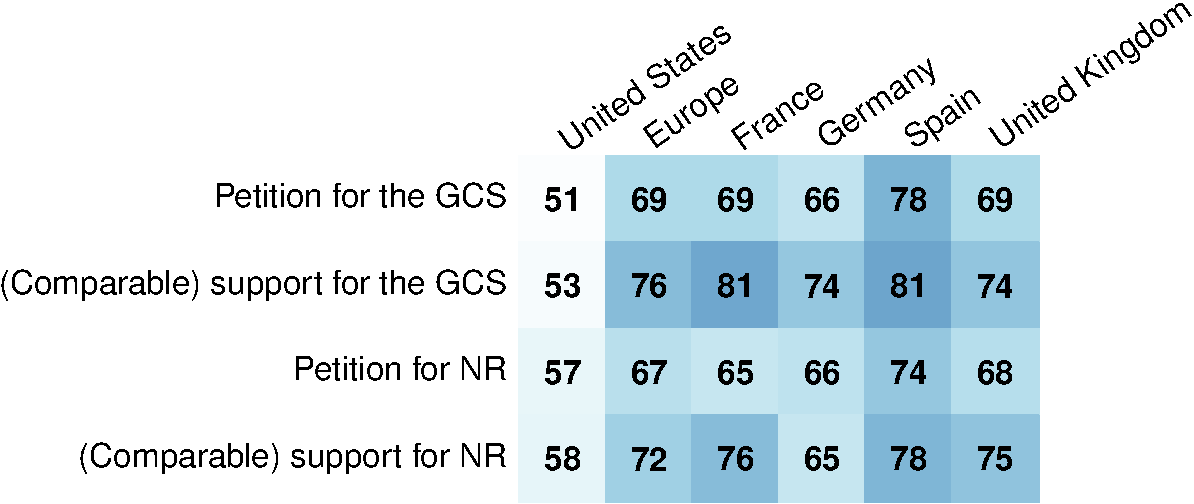
\includegraphics[width=.8\textwidth]{../figures/country_comparison/petition_comparable_positive.pdf}} 
\end{figure}

\begin{figure}[h!] % TODO? More details?
    \caption[Absolute support for various global policies]{Absolute support for various global policies (Percent of (\textit{somewhat} or \textit{strong}) support). (Questions \ref{q:climate_policies} and \ref{q:other_policies}. See Figure \ref{fig:support} for the relative support.)}\label{fig:support_likert_positive}
    \makebox[\textwidth][c]{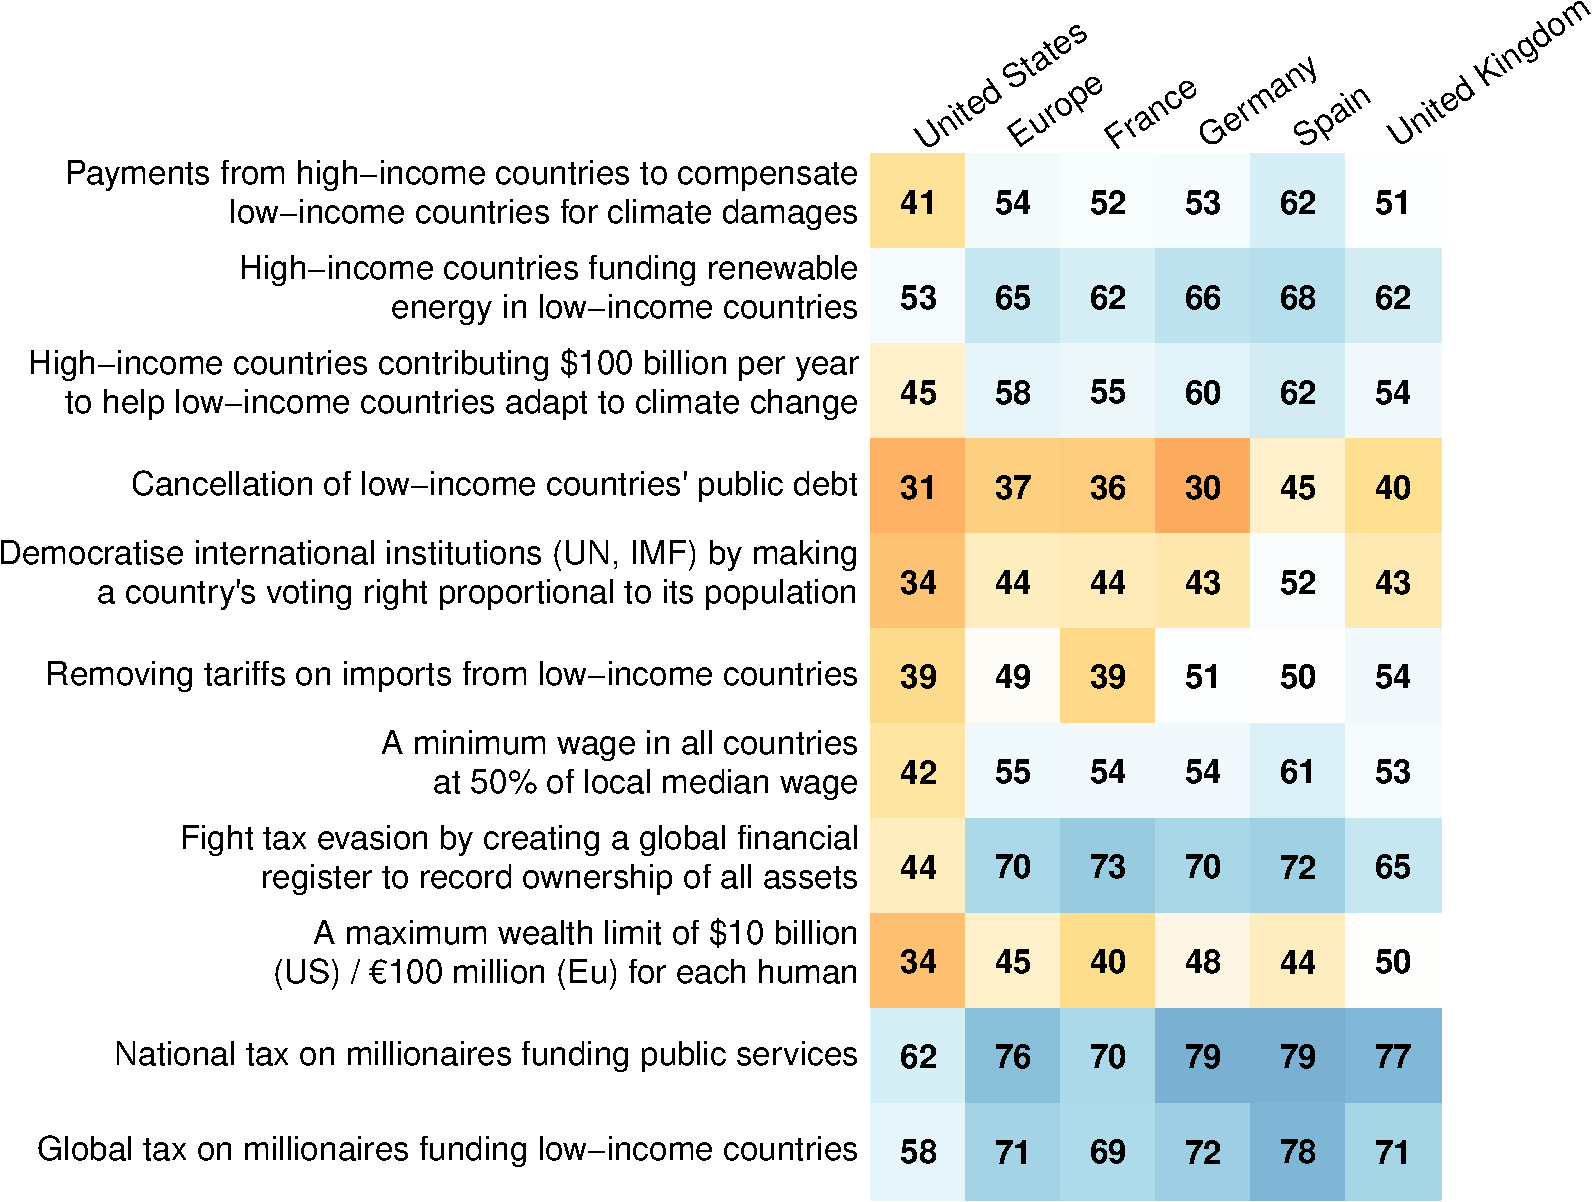
\includegraphics[width=\textwidth]{../figures/country_comparison/support_likert_positive.pdf}} 
\end{figure}

% \begin{figure}[h!]
%     \caption{label}\label{fig:climate_policies}
%     \makebox[\textwidth][c]{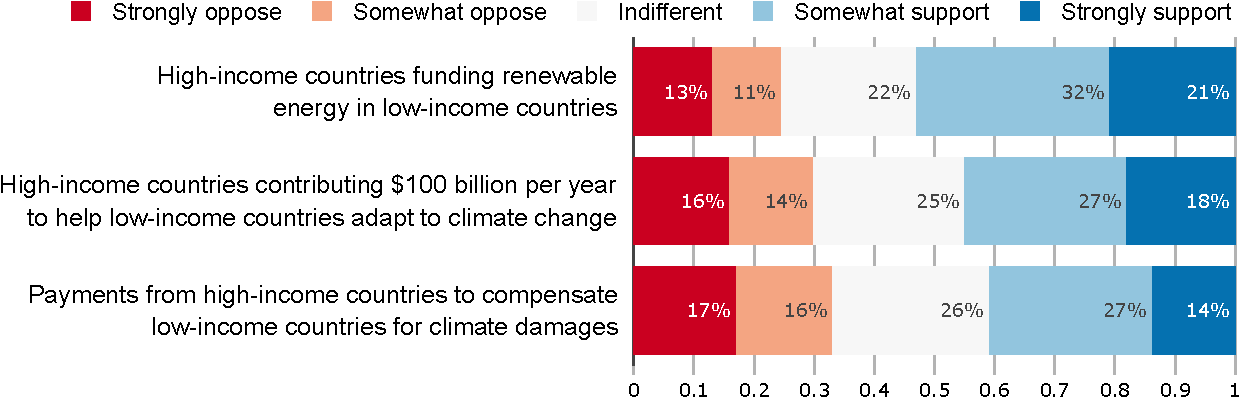
\includegraphics[width=\textwidth]{../figures/country_comparison/climate_policies.pdf}} 
% \end{figure}

% \begin{figure}[h!]
%     \caption{label}\label{fig:global_policies}
%     \makebox[\textwidth][c]{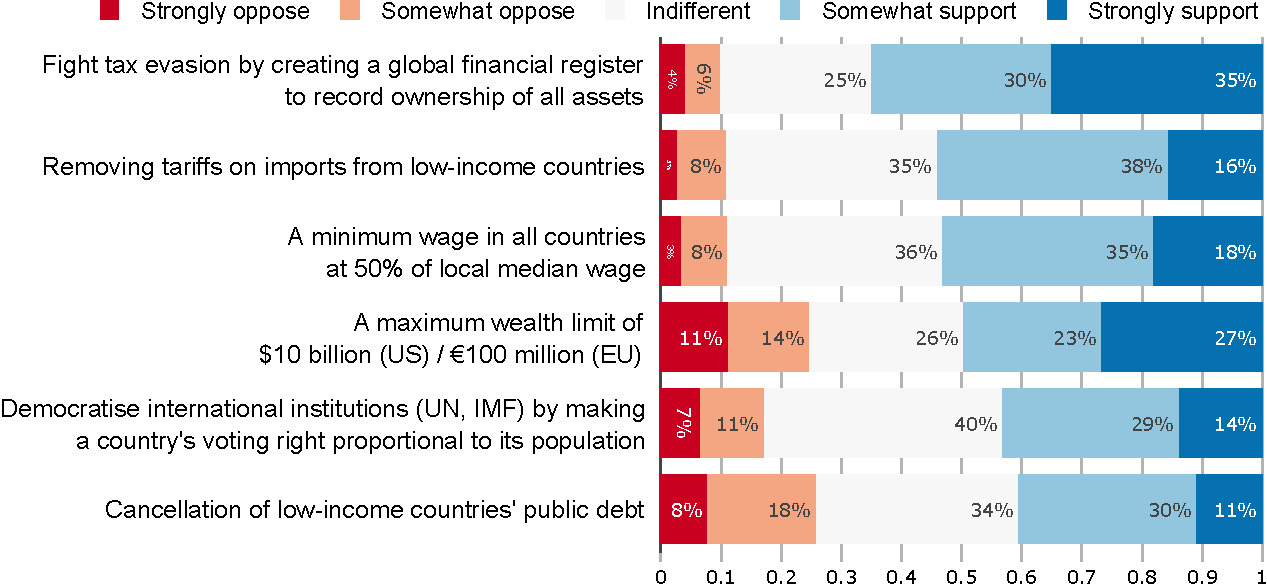
\includegraphics[width=\textwidth]{../figures/country_comparison/global_policies.pdf}} 
% \end{figure}

\begin{figure}[h!]
    \caption[Preferred approach for international climate negotiations]{Preferred approach of diplomats at international climate negotiations. \\ In international climate negotiations, would you prefer [U.S.] diplomats to defend [own country] interests or global justice? (Question \ref{q:negotiation})}\label{fig:negotiation}
    \makebox[\textwidth][c]{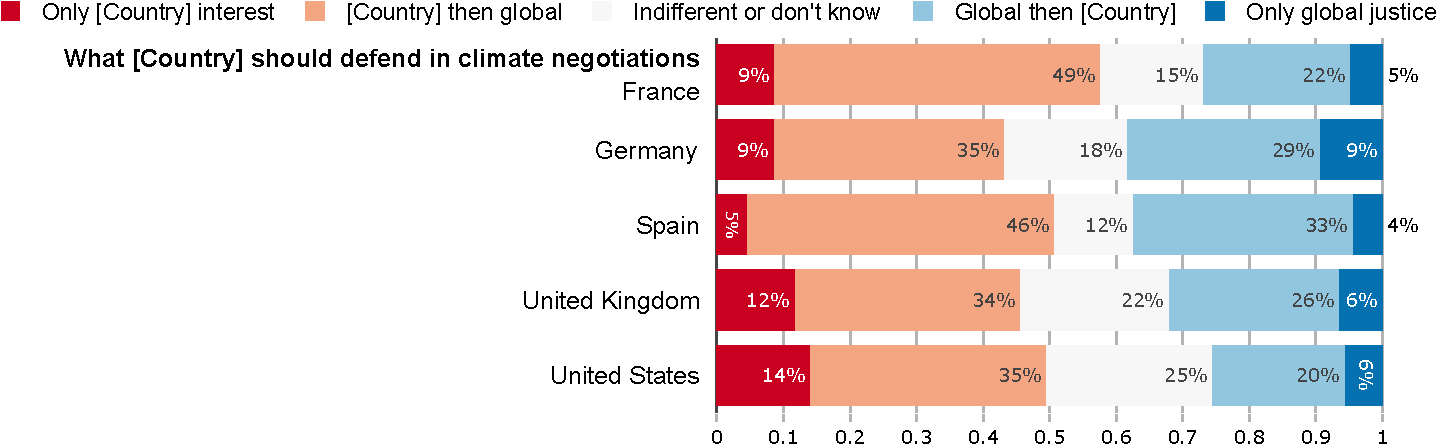
\includegraphics[width=\textwidth]{../figures/country_comparison/negotiation.pdf}} 
\end{figure}

\begin{figure}[h!]
    \caption[Importance of selected issues]{Percent of selected issues viewed as important.\\ ``To what extent do you think the following issues are a problem?'' (Question \ref{q:problem})}\label{fig:problem}
    \makebox[\textwidth][c]{
\includegraphics[width=.75\textwidth]{../figures/country_comparison/problem_positive.pdf}} 
\end{figure}

\begin{figure}[h!]
    \caption[Group defended when voting]{Group defended when voting. \\ ``What group do you defend when you vote?'' (Question \ref{q:group_defended})}\label{fig:group_defended}
    \makebox[\textwidth][c]{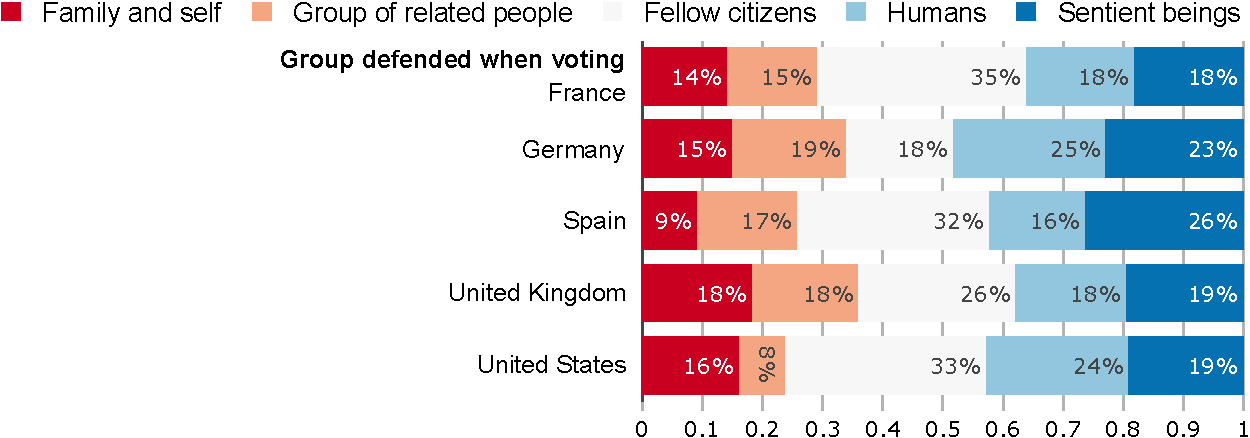
\includegraphics[width=\textwidth]{../figures/country_comparison/group_defended_agg2.pdf}} 
\end{figure}

% \begin{figure}[h!]
%     \caption{label}\label{fig:group_defended}
%     \makebox[\textwidth][c]{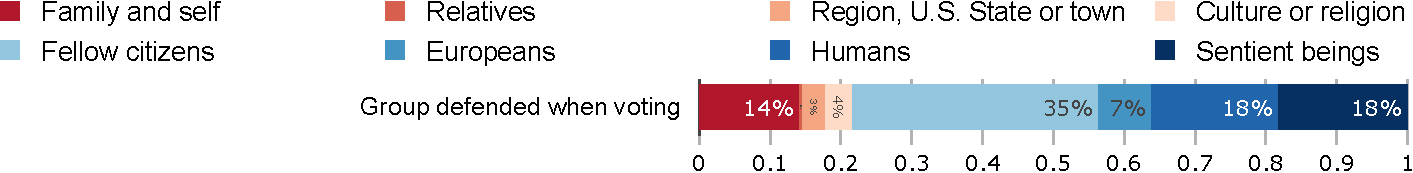
\includegraphics[width=\textwidth]{../figures/country_comparison/group_defended.pdf}} 
% \end{figure}

\begin{figure}[h!] 
    \caption[Mean prioritization of policies]{Mean prioritization of policies. \\Mean number of points allocated policies to express intensity of support (among six policies chosen at random). Blue color means that the policy has been awarded more points than the average policy. (Question \ref{q:points})}\label{fig:points}
    \makebox[\textwidth][c]{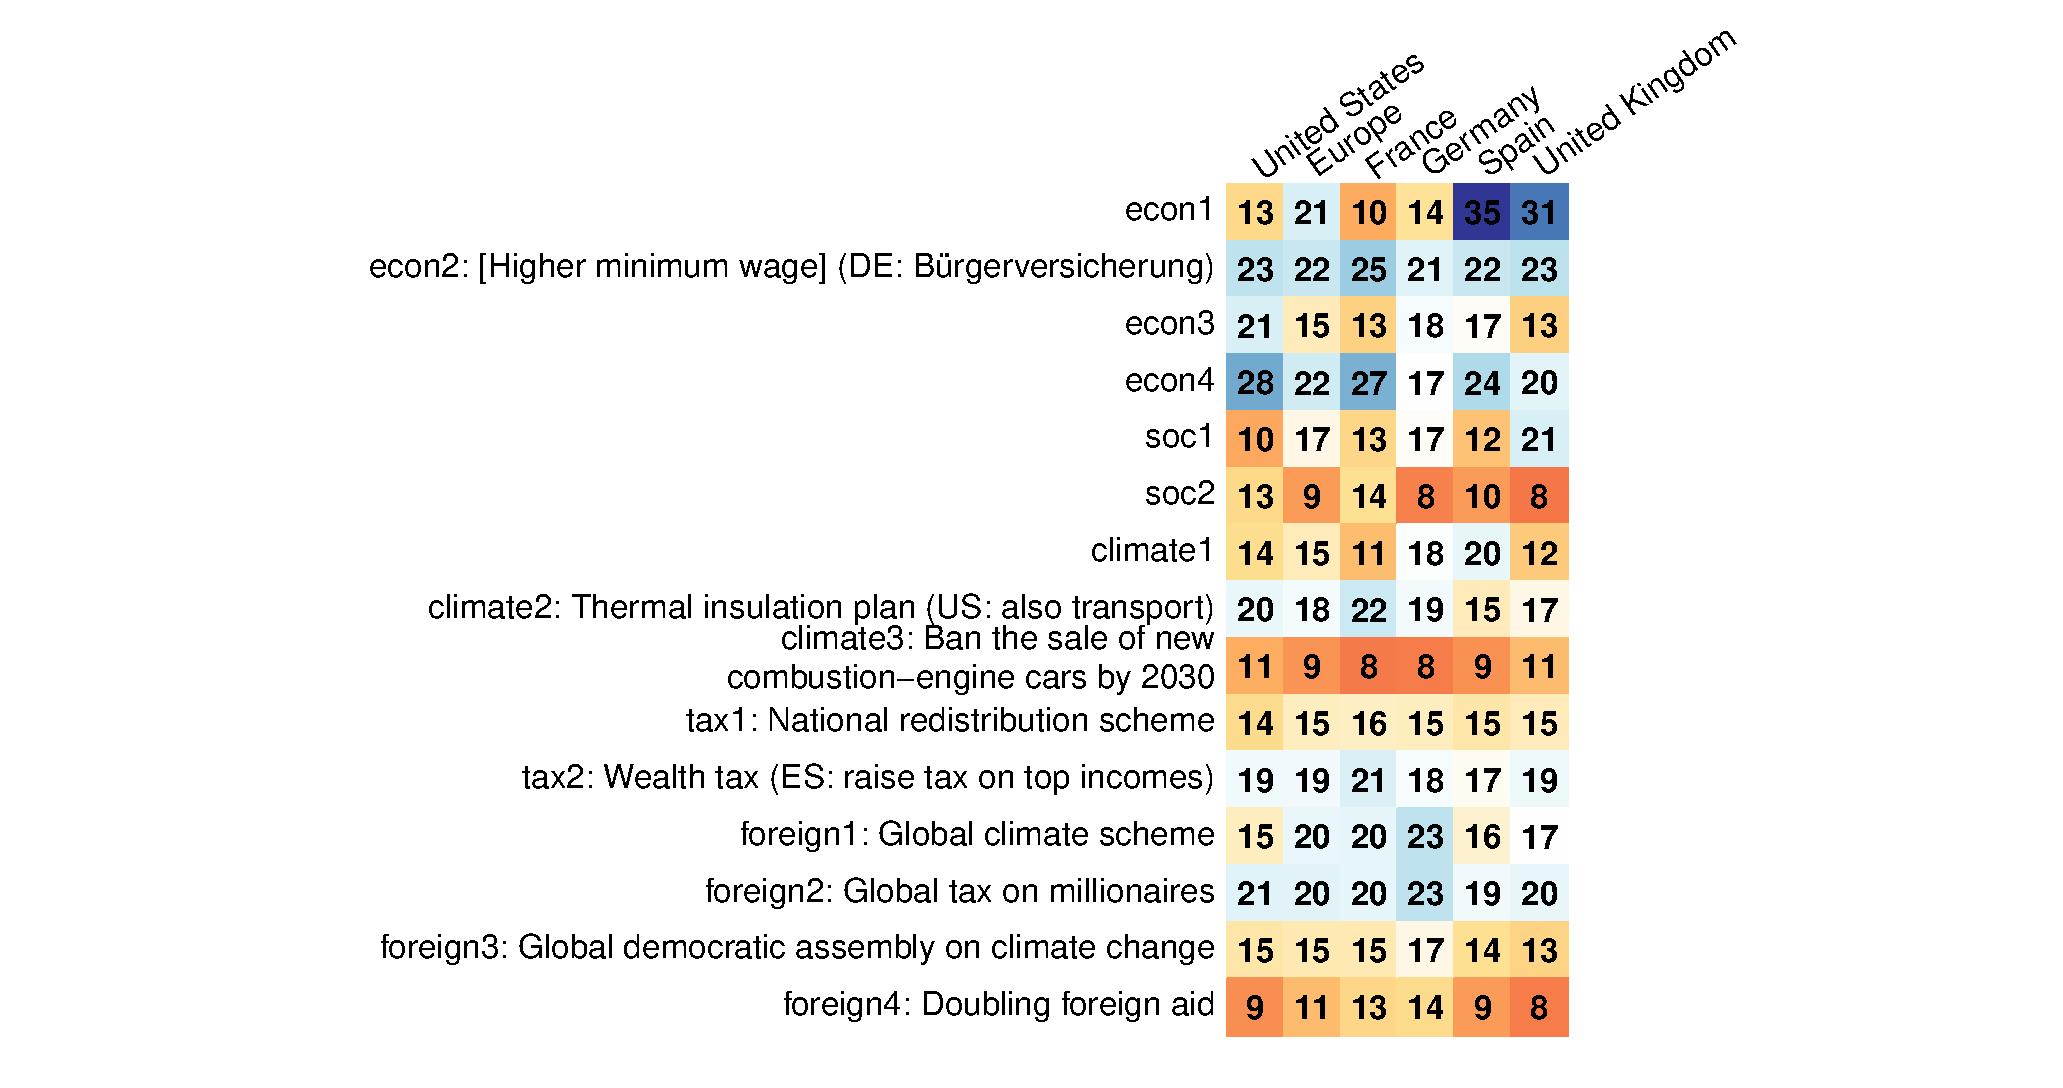
\includegraphics[width=\textwidth]{../figures/country_comparison/points_mean.pdf}} 
\end{figure}

\begin{figure}[h!] 
    \caption[Positive prioritization of policies]{Positive prioritization of policies. \\ Percent of people allocating a positive number of points to policies, expressing their support (among six policies chosen at random). (Question \ref{q:points})}\label{fig:points_positive}
    \makebox[\textwidth][c]{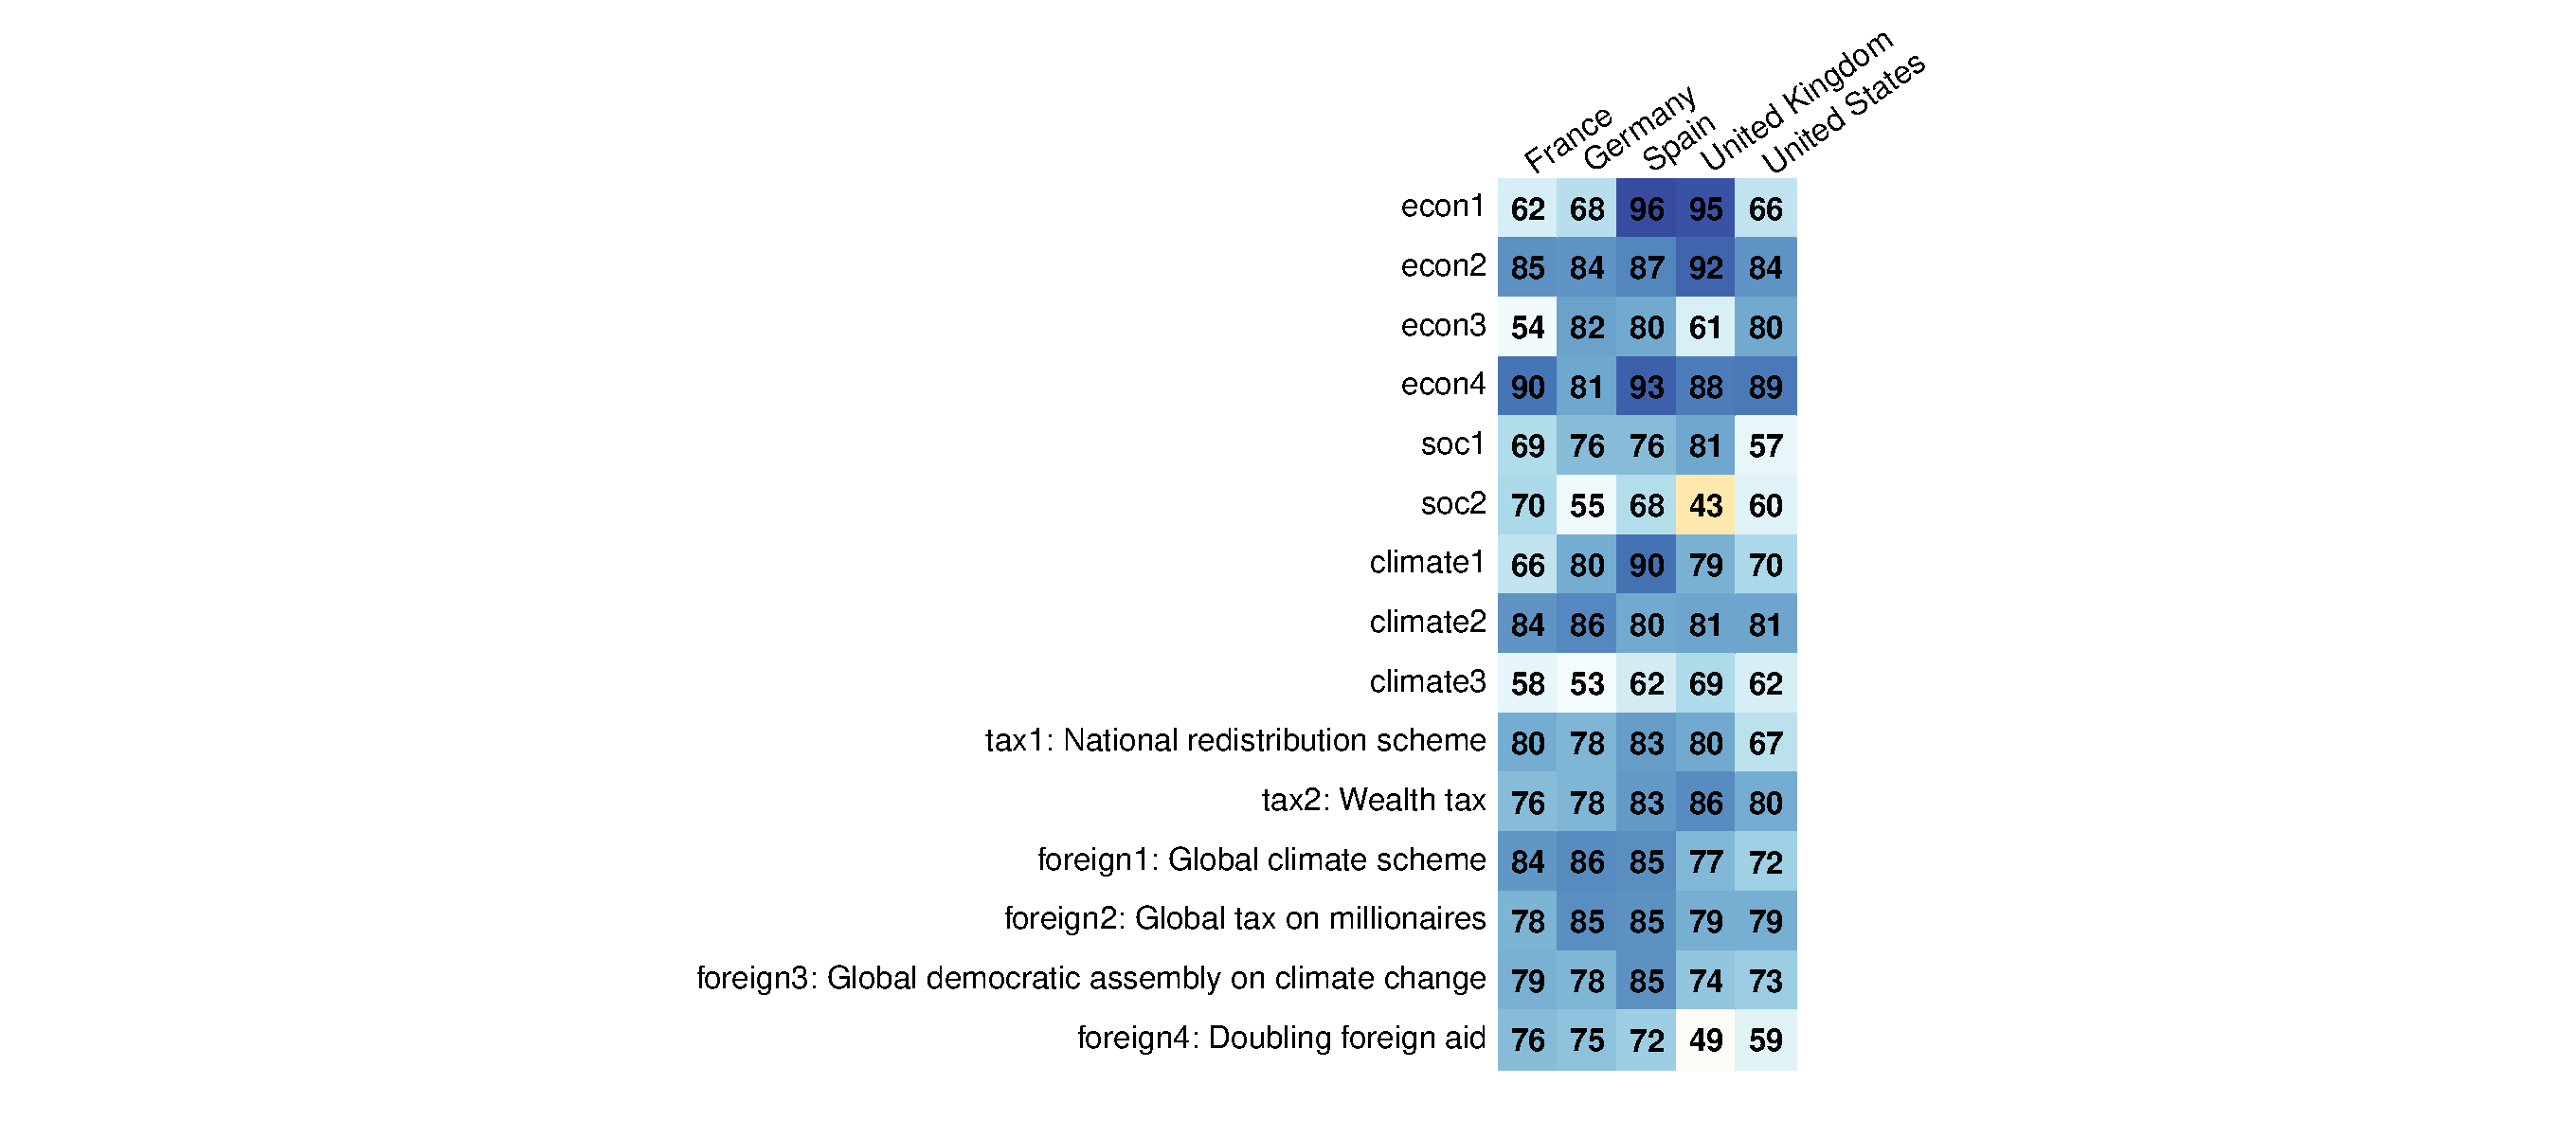
\includegraphics[width=\textwidth]{../figures/country_comparison/points_positive.pdf}} 
\end{figure}

\begin{figure}[h!]
    \caption[Charity donation]{Charity donation. \\ ``How much did you give to charities in 2022?'' (Question \ref{q:donation_charities})}\label{fig:donation_charities}
    \makebox[\textwidth][c]{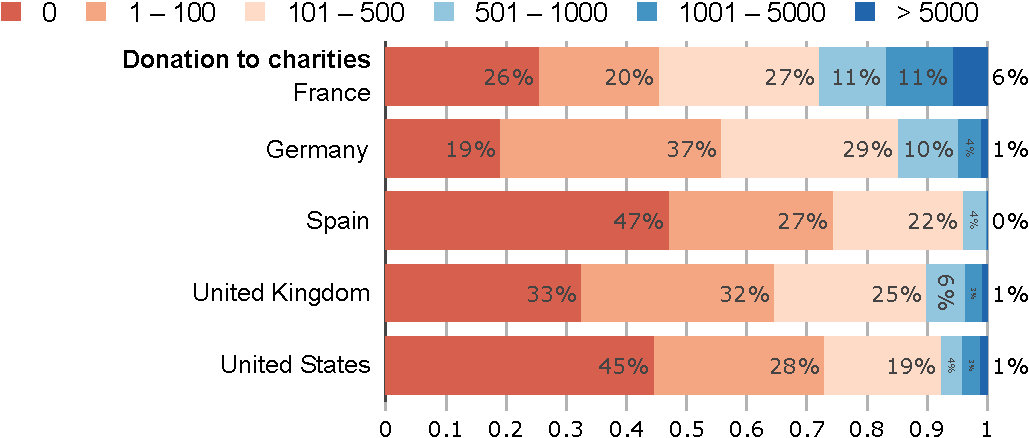
\includegraphics[width=.8\textwidth]{../figures/country_comparison/donation_charities.pdf}} 
\end{figure}

\begin{figure}[h!] 
    \caption[Interest in politics]{Interest in politics. \\ ``To what extent are you interested in politics?'' (Question \ref{q:interested_politics})}\label{fig:interested_politics}
    \makebox[\textwidth][c]{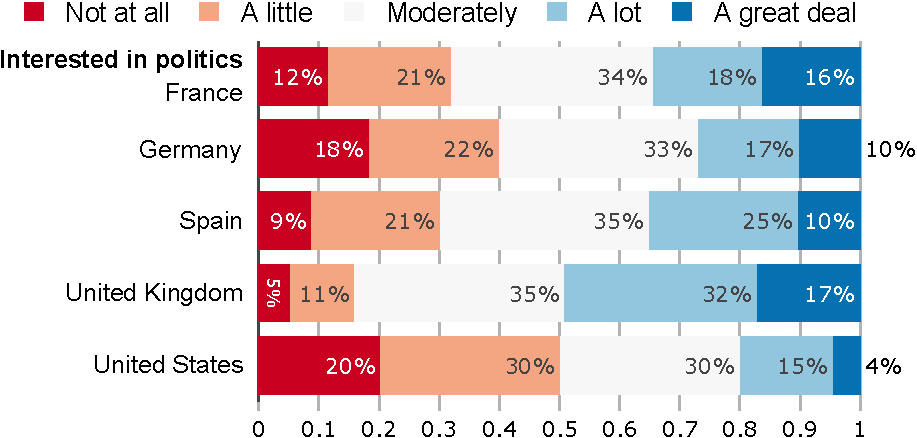
\includegraphics[width=.8\textwidth]{../figures/country_comparison/interested_politics.pdf}} 
\end{figure}

\begin{figure}[h!] 
    \caption[Desired involvement of government]{Desired involvement of government (from 1 to 5). (Question \ref{q:involvement_govt})}\label{fig:involvement_govt}
    \makebox[\textwidth][c]{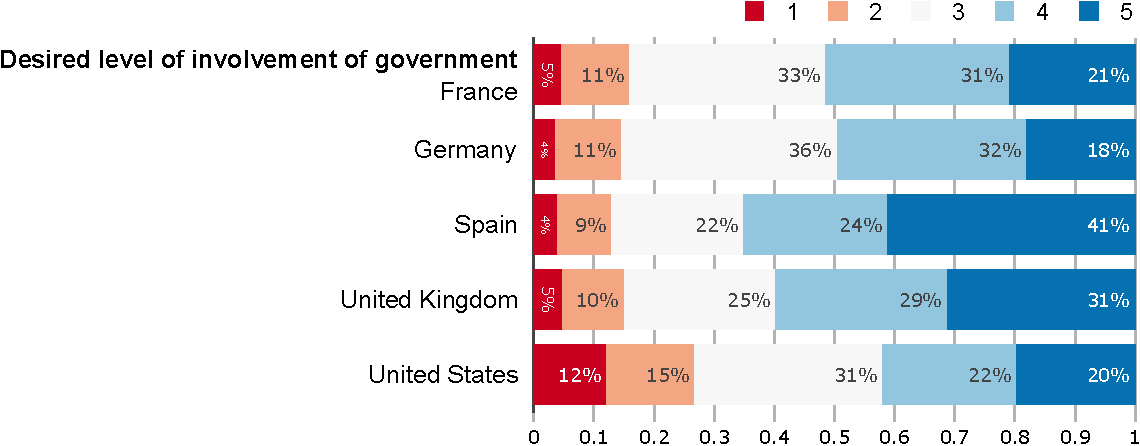
\includegraphics[width=.9\textwidth]{../figures/country_comparison/involvement_govt.pdf}} 
\end{figure}

\begin{figure}[h!] 
    \caption[Political leaning]{Political leaning on economics (from 1: Left to 5: Right). (Question \ref{q:left_right})}\label{fig:left_right}
    \makebox[\textwidth][c]{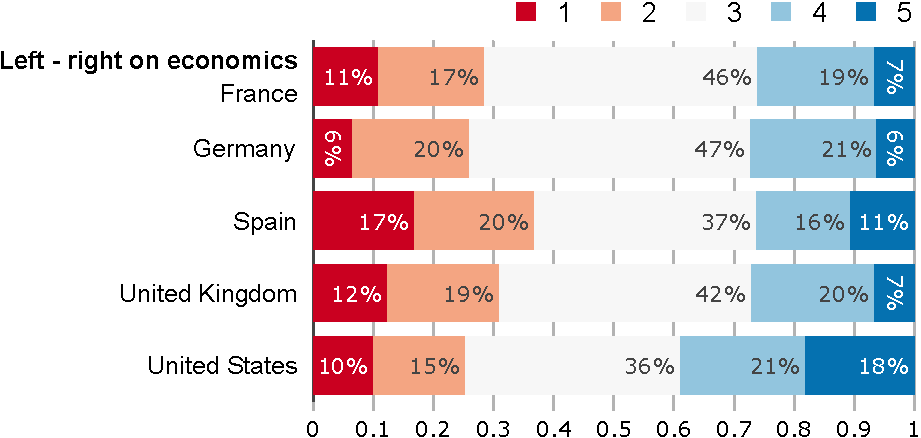
\includegraphics[width=.8\textwidth]{../figures/country_comparison/left_right.pdf}} 
\end{figure}

\begin{figure}[h!] 
    \caption[Voted in last election]{Voted in last election. (Question \ref{q:vote_participation})}\label{fig:vote_participation}
    \makebox[\textwidth][c]{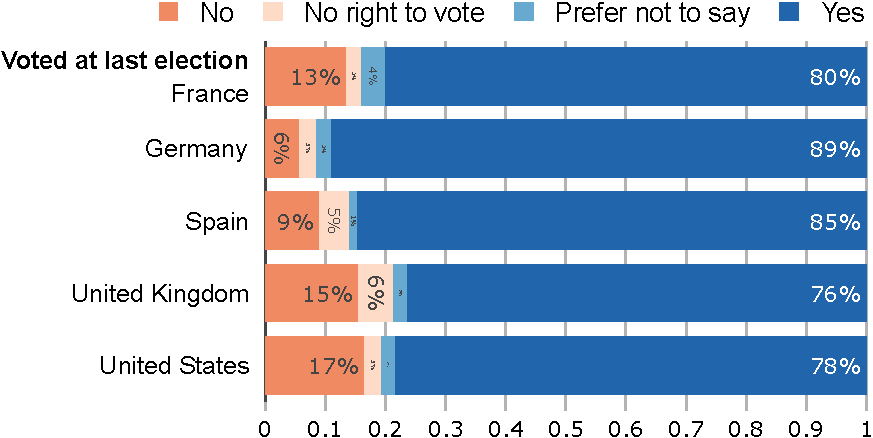
\includegraphics[width=.8\textwidth]{../figures/country_comparison/vote_participation.pdf}} 
\end{figure}

\begin{figure}[h!] 
    \caption[Vote in last election]{Vote in last election (aggregated). \textit{PNR} includes people who did not vote or prefer not to answer. (Question \ref{q:vote})}\label{fig:vote}
    \makebox[\textwidth][c]{\includegraphics[width=.75\textwidth]{../figures/country_comparison/vote.pdf}} 
\end{figure}

\begin{figure}[h!] 
    \caption[Perception that survey was biased]{Perception that survey was biased. \\ ``Do you feel that this survey was politically biased?'' (Question \ref{q:survey_biased})}\label{fig:survey_biased}
    \makebox[\textwidth][c]{\includegraphics[width=.7\textwidth]{../figures/country_comparison/survey_biased.pdf}} 
\end{figure}

% \begin{columns}
% \begin{column}{.5\textwidth}
% \begin{multicols}{2}
    \begin{figure}[h!]
        \caption[Classification of open-ended field on extreme poverty]{Opinion on the fight against extreme poverty. \\ ``According to you, what should high-income countries do to fight extreme poverty in low-income countries?'' (Question \ref{q:poverty_field})  \hfill (Back~to~Section~\ref{subsubsec:support_foreign_aid})}\label{fig:poverty_field}
    \begin{subfigure}{.34\textwidth}
        \caption{Elements found in the open-ended field on the question (manually recoded, in percent)}.
        \includegraphics[width=\textwidth]{../figures/country_comparison/poverty_field_positive.pdf}        
    \end{subfigure}
    \hspace{.02\textwidth}
    \begin{subfigure}{.64\textwidth}
        \caption{Keywords found in the open-ended field on the GCS (automatic search ignoring case, in percent).}
        \includegraphics[width=\textwidth]{../figures/country_comparison/poverty_field_contains_positive.pdf}    
    \end{subfigure}
    \end{figure}
% \end{column}
% \begin{column}{.5\textwidth}
    % \begin{figure}[h!]
    %     \caption[Topics of open-ended field on extreme poverty]{Opinion on the fight against extreme poverty. \\ ``According to you, what should high-income countries do to fight extreme poverty in low-income countries?'' \\ Keywords found in the open-ended field on the GCS (automatic search ignoring case, in percent). (Question \ref{q:poverty_field})}\label{fig:poverty_field_contains}
    %     \makebox[\textwidth][c]{\includegraphics[width=\columnwidth]{../figures/country_comparison/poverty_field_contains_positive.pdf}} 
    % \end{figure}
% \end{multicols}
% \end{column}
% \end{columns}


\begin{figure}[h!] 
    \caption[Main attitudes by vote]{Main attitudes by vote (``Right'' spans from Center-right to Far right). \\ (Relative support in percent in Questions \ref{q:gcs_support}, \ref{q:global_tax}, \ref{q:other_policies}, \ref{q:foreign_aid_raise_support}, \ref{q:negotiation}) \hfill (Back~to~Section~\ref{subsec:universalistic})}\label{fig:main_by_vote}
    \makebox[\textwidth][c]{\includegraphics[width=\textwidth]{../figures/country_comparison/main_all_by_vote_share.pdf}} 
\end{figure}

% \begin{figure}[h!] 
%     \caption[Interested to be interviewed]{Interested to be interviewed by a researcher for 30 min through videoconference. (Question \ref{q:interview})}\label{fig:interview}
%     \makebox[\textwidth][c]{\includegraphics[width=\textwidth]{../figures/country_comparison/interview.pdf}} 
% \end{figure}    

% \begin{figure}[h!]
%     \caption{label}\label{fig:share_policies_supported}
%     \makebox[\textwidth][c]{\includegraphics[width=\textwidth]{../figures/country_comparison/share_policies_supported.pdf}} 
% \end{figure} % TODO? uncomment?

% \begin{figure}[h!]
%     \caption{label}\label{fig:vars}
%     \makebox[\textwidth][c]{\includegraphics[width=\textwidth]{../figures/country_comparison/vars.pdf}} 
% \end{figure}

% In Denmark, France and the U.S., the questions with an asterisk were asked differently, asking ``To achieve a given reduction of greenhouse gas emissions globally, costly investments are needed. Ideally, how should countries bear the costs of fighting climate change?''. Instead of the equal right per capita, the item was ``Countries should pay in proportion to their current emissions'', historical responsibilities was worded as ``Countries should pay in proportion to their past emissions (from 1990 onwards)'', then there was an item ``The richest countries should pay it all'', and compensating vulnerable countries was worded as ``The richest countries should pay even more, to help vulnerable countries face adverse consequences: vulnerable countries would then receive money instead of paying''.

\clearpage 
\section{Questionnaire of the global survey (section on global policies)}\label{app:questionnaire_oecd}
%\subsection*{International burden-sharing}
\renewcommand{\theenumi}{\Alph{enumi}}
\begin{enumerate} \item \label{q:scale} At which level(s) do you think public policies to tackle climate change need to be put in place? (Multiple answers are possible) [\textit{Figures \ref{fig:oecd} and \ref{fig:oecd_absolute}}]
\\ \textit{Global; [Federal / European / ...]; [State / National]; Local}
\item Do you agree or disagree with the following statement: ``[country] should take measures to fight climate change.''% TODO! figure
	\\ \textit{Strongly disagree; Somewhat disagree; Neither agree nor disagree; Somewhat agree; Strongly agree}
\item How should [country] climate policies depend on what other countries do?% TODO! figure
 \begin{itemize}
\item If other countries do more, [country] should do...
\item If other countries do less, [country] should do...
\end{itemize}
\textit{Much less; Less; About the same; More; Much more}
\item ~[In all countries but the U.S., Denmark and France]  All countries have signed the Paris agreement that aims to contain global warming ``well below +2 \textdegree{}C\''. To limit global warming to this level, there is a maximum amount of greenhouse gases we can emit globally, called the carbon budget. Each country could aim to emit less than a share of the carbon budget. To respect the global carbon budget, countries that emit more than their national share would pay a fee to countries that emit less than their share. \\ 
Do you support such a policy? [\textit{Figures \ref{fig:oecd} and \ref{fig:oecd_absolute}}]
\\ \textit{Strongly oppose; Somewhat oppose; Neither support nor oppose; Somewhat support; Strongly support}
\item ~[In all countries but the U.S., Denmark and France] Suppose the above policy is in place. How should the carbon budget be divided among countries? [\textit{Figures \ref{fig:oecd} and \ref{fig:oecd_absolute}}]
\\ \textit{The emission share of a country should be proportional to its population, so that each human has an equal right to emit.; The emission share of a country should be proportional to its current emissions, so that those who already emit more have more rights to emit.; Countries that have emitted more over the past decades (from 1990 onwards) should receive a lower emission share, because they have already used some of their fair share.; Countries that will be hurt more by climate change should receive a higher emission share, to compensate them for the damages.}
\item \label{q:burden_sharing_asterisk} ~[In the U.S., Denmark, and France only] To achieve a given reduction of greenhouse gas emissions globally, costly investments are needed. % TODO! figure
Ideally, how should countries bear the costs of fighting climate change?
 \begin{itemize}
\item Countries should pay in proportion to their income
\item Countries should pay in proportion to their current emissions [Used as a substitute to the equal right per capita in Figure \ref{fig:oecd}]
\item Countries should pay in proportion to their past emissions (from 1990 onwards) [Used as a substitute to historical responsibilities in Figure \ref{fig:oecd}]
\item The richest countries should pay it all, so that the poorest countries do not have to pay anything
\item The richest countries should pay even more, to help vulnerable countries face adverse consequences: vulnerable countries would then receive money instead of paying [Used as a substitute to compensating vulnerable countries in Figures \ref{fig:oecd} and \ref{fig:oecd_absolute}]
\end{itemize} 
\textit{Strongly disagree; Somewhat disagree; Neither agree nor disagree; Somewhat agree; Strongly agree}
\item Do you support or oppose establishing a global democratic assembly whose role would be to draft international treaties against climate change? Each adult across the world would have one vote to elect members of the assembly. [\textit{Figures \ref{fig:oecd} and \ref{fig:oecd_absolute}}]
\\ \textit{Strongly oppose; Somewhat oppose; Neither support nor oppose; Somewhat support; Strongly support}
\item Imagine the following policy: a global tax on greenhouse gas emissions funding a global basic income. 
Such a policy would progressively raise the price of fossil fuels (for example, the price of gasoline would increase by [40 cents per gallon] in the first years). Higher prices would encourage people and companies to use less fossil fuels, reducing greenhouse gas emissions. Revenues from the tax would be used to finance a basic income of [\$30] per month to each human adult, thereby lifting the 700 million people who earn less than \$2/day out of extreme poverty. 
The average [American] person would lose a bit from this policy as they would face [\$130] per month in price increases, which is higher than the [\$30] they would receive.

Do you support or oppose such a policy?  [\textit{Figures \ref{fig:oecd} and \ref{fig:oecd_absolute}}]
\\ \textit{Strongly oppose; Somewhat oppose; Neither support nor oppose; Somewhat support; Strongly support}
\item \label{q:millionaire_tax} Do you support or oppose a tax on all millionaires around the world to finance low-income countries that comply with international standards regarding climate action? 
This would finance infrastructure and public services such as access to drinking water, healthcare, and education. [\textit{Figures \ref{fig:oecd} and \ref{fig:oecd_absolute}}]
\\ \textit{Strongly oppose; Somewhat oppose; Neither support nor oppose; Somewhat support; Strongly support}
\end{enumerate}

% \clearpage
% \section{Questionnaire of US1 %the first U.S. complementary 
% survey}\label{app:questionnaire_US1}

% \begin{figure}[h!]
%     \caption{US1 survey structure}\label{fig:flow_US1}
%     \makebox[\textwidth][c]{\includegraphics[width=\textwidth]{../questionnaire/survey_flow_US1.pdf}} 
% \end{figure}

\renewcommand{\theenumi}{\arabic{enumi}}
\clearpage
\section{Questionnaire of the complementary surveys}\label{app:questionnaire}
% /!\ Ctrl+H "\item ~[" / "\\ ["=> "\item ~[" / "\\ ~["
% TODO!? put in italic the "didascalies" in []
% TODO? give policies options here instead of referring to "this spreadsheet"
Below, we provide the generic questionnaire (based on the U.S. version), which roughly corresponds to the \textit{Eu} questionnaire as well as the combination of the \textit{US1} and \textit{US2} questionnaire. The main difference between Europe and the U.S. is that we split the \textit{US2} sample into four random branches to include some treatments before the Section \ref{subsec:questionnaire_GCS} on the GCS. Besides the control group, the treatments are: information regarding the support of Americans for the GCS and NR, an open-ended field, and a closed question on the pros and cons of the GCS. The pros and cons of the GCS are also asked in \textit{Eu} (likewise, either as an open-ended field or a question), but only in Section \ref{subsec:questionnaire_perceptions}, after the support. 

At each section or question, square brackets specify in which questionnaires it is present (\textit{US1}, \textit{US2} and/or \textit{Eu}) as well as country specificities. Figures \ref{fig:flow_Eu}-\ref{fig:flow_US2} display the structure of each questionnaire. Each treatment randomization is independent. Qualtrics and Word versions of the questionnaires in each language are available on our \href{https://github.com/bixiou/international_attitudes_toward_global_policies/tree/main/questionnaire}{public repository}, together with a spreadsheet that summarizes country specificities and our sources.

\begin{figure}[h!]
    \caption{\textit{Eu} survey structure}\label{fig:flow_Eu}
    \makebox[\textwidth][c]{\includegraphics[width=\textwidth]{../questionnaire/survey_flow_EU.pdf}} 
\end{figure}

\begin{figure}[h!]
    \caption{\textit{US1} survey structure}\label{fig:flow_US1}
    \makebox[\textwidth][c]{\includegraphics[width=\textwidth]{../questionnaire/survey_flow_US1.pdf}} 
\end{figure}

\begin{figure}[h!]
    \caption{\textit{US2} survey structure}\label{fig:flow_US2}
    \makebox[\textwidth][c]{\includegraphics[width=\textwidth]{../questionnaire/survey_flow_US2.pdf}} 
\end{figure}

\clearpage
\subsection*{[\textit{Eu}, \textit{US1}, \textit{US2}] Socio-demographic characteristics}
\begin{enumerate}
\item Welcome to this survey!\\
\\
This survey is \textbf{anonymous} and is conducted \textbf{for research} purposes on a representative sample of [1,000 British people].\\
 \\
It takes [\textit{US1}, \textit{US2}: 10 to 15 min; \textit{Eu}: around \textbf{20 min}] to complete.  \\
 \\
The survey contains lotteries and awards for those who get the correct answer to some understanding questions.\\
If you are attentive and lucky, \textbf{you can win up to }[\textit{US1}, \textit{Eu}: \textbf{\$350}; \textit{US2}: \textbf{\$150}] in points. (\href{https://uvafeb.eu.qualtrics.com/WRQualtricsControlPanel/File.php?F=F_cBZAXTgNktGZbee&download=1}{See terms and conditions}).    \\
Please answer every question carefully.  \\
 \\
\textbf{Do you agree to participate in the survey?}
\\ \textit{Yes; No}
\item What is your gender?
\\ \textit{Woman; Man; Other}
\item How old are you?
\\ \textit{Below 18; 18 to 20; 21 to 24; 25 to 29; 30 to 34; 35 to 39; 40 to 44; 45 to 49; 50 to 54; 55 to 59; 60 to 64; 65 to 69; 70 to 74; 75 to 79; 80 to 84; 85 to 89; 90 to 99; 100 or above}
\item ~[\textit{Eu}] In which country do you live?
\\ \textit{France; Germany; Spain; United Kingdom; Other}
\item What is your ZIP code? [UK: What is your Outcode (the left part of your postcode, e.g. if your postcode is N7 8H7, just enter N7)?]
\item \label{q:partner} Do you live with your partner (if you have one)?
\\ \textit{Yes; No}
\item How many people are in your household? The household includes: you, the members of your family who live with you, and your dependants. %This excludes flatmates.
\\ \textit{1; 2; 3; 4; 5 or more}
\item \label{q:children} [\textit{Eu}] How many children below 14 live with you?
\\ \textit{1; 2; 3; 4 or more}
\item ~[\textit{US1}, \textit{US2}] What race or ethnicity do you identify with? (Multiple answers are possible) 
\\ \textit{White; Black or African American; Hispanic; Asian; American Indian or Alaskan Native; Natice Hawaiian or Pacific Islander; Other: \{open field\}; Prefer not to say}
\item What is the [\textit{US1}, \textit{US2}: \textit{annual}; \textit{Eu}: \textit{monthly}] gross income of your household (before withholding tax)? This includes all income: wages, self-employment earnings, Social Security benefits, pensions, investment income, welfare payments, and income from other sources. % ~[quartiles thresholds are given for the U.S. ] 
\\ ~[\textit{US1}, \textit{US2}: Items based on household total income deciles and quartiles, namely: \textit{Less than \$20,000; between \$20,001 and \$35,000; between \$35,001 and \$42,000; between \$42,001 and \$50,000; between \$50,001 and \$65,000; between \$65,001 and \$82,000; between \$82,001 and \$103,000; between \$103,001 and \$130,000; between \$130,001 and \$145,000; between \$145,001 and \$165,000; between \$165,001 and \$250,000; More than \$250,000; I prefer not to answer}; \\ \textit{Eu}: custom thresholds, taking into account household composition Questions \ref{q:partner}-\ref{q:children}, and corresponding to the country's deciles and quartiles of standard of living, cf. the sheet ``Income'' in \href{https://github.com/bixiou/international_attitudes_toward_global_policies/raw/main/questionnaire/specificities.xlsx}{this spreadsheet}]
\item What is the highest level of education you have completed? 
\\ ~[\textit{Below upper secondary}, \textit{Upper secondary}, and \textit{Post secondary} are coded as the first two, middle three, and last three items, respectively. \\ \textit{US1}, \textit{US2}: \textit{Primary school or less; Eigth grade; Some high school; Regular high school diploma/GED or alternative credential; Some college, no degree; 2-year college degree or associates degree (for example: AA, AS); Bachelor's degree (for example: BA, BS); Master’s degree or above (MA, MS, MEng, MEd, MSW, MBA, MD, DDS, DVM, LLB, JD, PhD); } \\FR: \textit{École primaire / Aucun; Brevet; CAP ou BEP; Baccalauréat professionnel ou technologique; Baccalauréat général; Bac +2 (BTS, DUT, DEUG…); Bac +3 (licence…); Bac +5 ou plus (master, école d'ingénieur ou de commerce, doctorat, médecine, maîtrise, DEA, DESS...)} \\DE: \textit{Keine abgeschlossene Schulbildung / Grundschule; Untere Sekundarstufe (z.B. Haupt- oder Realschulabschluss); Erstausbildung; Beruflicher Abschluss / Ausbildung; Abitur; Zweitausbildung; Bachelor oder Fachhochschulabschluss; Master-Abschluss oder höher} \\ ES: \textit{Educación primaria / No he completado la enseñanza básica; Educación secundaria obligatoria (ESO); Formación profesional básica (FP); Formación profesional de grado medio; Bachillerato; Formación profesional de grado superior; Grado universitario; Máster/doctorado}\\ UK: \textit{Primary education or less; Some secondary school; GSCE; Vocational Upper secondary (Level 3 award, level 3 certificate, level 3 diploma, advanced apprenticeship, etc.); High school degree (A level); Higher vocational education (Level 4+ award, level 4+ certificate, level 4+ diploma, higher apprenticeship, etc.); Bachelor's Degree (BA, BSc, BEng, etc.); Postgraduate diploma or certificate, Master's Degree (MSc, MA, MBA, etc.) or Ph.D.}]
\item What is your employment status? \label{item:employment}
\\ \textit{Full-time employed; Part-time employed; Self-employed; Student; Retired; Unemployed (searching for a job); Inactive (not searching for a job)}
\item Are you a homeowner or a tenant? (Multiple answers are possible) 
\\ \textit{Tenant; Owner; Landlord renting out property; Hosted free of charge}
\item ~[If lives with partner: What is the estimated value of your household's assets (in U.S. dollars)?  \\
 If does not live with partner: What is the estimated value of your assets (in U.S. dollars)?]
   \\
Include here all your possessions (home, car, savings, etc.) net of debt. For example, if you own a house worth [\$]300,000 and you have [\$]100,000 left to repay on your mortgage, your assets are [\$]200,000.  \\
  \\
I estimate my [If lives with partner: household's] assets net of debt to be:  \\% ~[Quintiles thresholds are given for the U.S. ]
% \\ ~[Items based on wealth quintiles. US1, \textit{US2}: \textit{Less than \$0 (I have a net debt); Close to \$0; Between \$4,000 and \$120,000; Between \$120,000 and \$380,000; More than \$380,000}; For Eu, the thresholds are: FR: \euro{}10/100/300/600k; DE: \euro{}0/70/260/560k; ES: \euro{}0/100/200/400k; UK: £6/90/230/530k] 
\\ ~[Items based on the following individual wealth quintiles, doubled if lives with partner. \textit{US1}, \textit{US2}: \textit{Less than \$0 (I have a net debt); Close to \$0; Between \$4,000 and \$60,000; Between \$60,000 and \$190,000; More than \$190,000}; For \textit{Eu}, the thresholds are: FR: \euro{}5/50/150/300k; DE: \euro{}0/35/130/280k; ES: \euro{}0/50/100/200k; UK: £3/45/115/270k] 
% \item ~[Asked if does not live with partner] What is the estimated value of your assets (in U.S. dollars)?   \\
%    \\
% Include here all your possessions (home, car, savings, etc.) net of debt. For example, if you own a house worth [\$]300,000 and you have [\$]100,000 left to repay on your mortgage, your assets are [\$]200,000.  \\
%   \\
%   I estimate my assets net of debt to be: \\% ~[Quintiles thresholds are given for the U.S. ]
% \\ ~[Items based on wealth quintiles. US1, \textit{US2}: \textit{Less than \$0 (I have a net debt); Close to \$0; Between \$4,000 and \$60,000; Between \$60,000 and \$190,000; More than \$190,000}; For Eu, the thresholds are: FR: \euro{}5/50/150/300k; DE: \euro{}0/35/130/280k; ES: \euro{}0/50/100/200k; UK: £3/45/115/270k] 
\item \label{q:political_affiliation} ~[\textit{US1}, \textit{US2} (where it is instead asked toward the end, after the vote question)] What do you consider to be your political affiliation, as of today?
\\ \textit{Republican; Democrat; Independent; Other; Non-Affiliated}
\end{enumerate}

\subsection*{[\textit{Eu}, \textit{US1}, \textit{US2}] Global climate scheme}\label{subsec:questionnaire_GCS}
\begin{enumerate}[resume] \item[] In the following, we describe two policies, on which we will survey your opinion. To check that you have attentively read the descriptions,~\textbf{we will ask some understanding questions afterwards: those who get correct answers can win up to \$150}. \\
\textbf{\underbar{Global climate scheme:}}~ At the Paris agreement in 2015, all countries have agreed to contain global warming ``well below +2 $\mathrm{{}^\circ}$C''. To limit global warming to this level,~\textbf{there is a maximum amount of greenhouse gases we can emit globally}.\\
To meet the climate target, a limited number of permits to emit greenhouse gases can be created globally. Polluting firms would be required to buy permits to cover their emissions. Such a policy would~\textbf{make fossil fuel companies pay}~for their emissions and progressively raise the price of fossil fuels.~\textbf{Higher prices would encourage people and companies to use less fossil fuels, reducing greenhouse gas emissions.}\\
In accordance with the principle that each human has an equal right to pollute, the revenues generated by the sale of permits could finance a global basic income.~\textbf{Each adult in the world would receive } [\textit{US1}, \textit{US2}: \textbf{\$30/month}; UK: \textbf{\$30 (that is £25) per month}; FR, DE, ES:  \textbf{\euro{}30/month}], thereby lifting out of extreme poverty the 700 million people who earn less than \$2/day.\\
\textbf{The typical }[\textbf{American}]\textbf{ would lose out financially }[\textit{US1}, \textit{US2}: \textbf{\$85}, FR: \textbf{\euro{}10}, DE: \textbf{\euro{}25}, ES: \textbf{\euro{}5}, UK: \textbf{£20}]\textbf{ per month}~(as he or she would face [\$115] per month in price increases, which is higher than the [\$30] they would receive). 
\\The policy could be put in place as soon as countries totaling more than 60\% of global emissions agree on it. Countries that would refuse to take part in the policy could face sanctions (like tariffs) from the rest of the World and would be excluded from the basic income. \hfill (Back~to~Section~\ref{subsubsec:global_support})
\item \label{q:understood_gcs} Who would win or lose financially in the Global climate scheme? [\textit{Figure \ref{fig:understood_each}}] \\
\\
Three respondents with the expected answer will get [\$]50 in points.
\\ \textit{Typical [Americans] would win and the 700 million poorest humans would win.; \\Typical [Americans] would win and the 700 million poorest humans would lose.; \\Typical [Americans] would lose and the 700 million poorest humans would win.; \\Typical [Americans] would lose and the 700 million poorest humans would lose.}
\item[[new page\!\!\!]] For your information, the expected answer was \textit{Typical [Americans] would lose and the 700 million poorest humans would win} from the Global climate scheme. Now, here is the second policy: \\ 
\\
\textbf{\underbar{National redistribution scheme:}}\\ This policy would \textbf{increase taxes on the top} [\textit{US1}, \textit{US2}: \textbf{5\%}; 
\textit{Eu}: \textbf{1\%}] and provide cash transfers to all adults. More precisely, \textbf{each }[\textbf{American}]\textbf{ adult would receive }[\textbf{\$85}]\textbf{ per month} (that is [\$1,000] per year). 
This would be financed by an increase of the federal income tax on household income in excess of [\textit{US1}, \textit{US2}: \$315,000 per year; FR: \euro{}15,000 per month; DE: \euro{}20,000 per month; ES: \euro{}10,000 per month; UK: £15,000 per month], leaving taxes unchanged for income below [\$315,000]. [\textit{US1}, \textit{US2}: \underbar{See more details}.]
\footnote{8\% of U.S. respondents click. They then see the following text, based on \href{https://taxjusticenow.org/\#makeYourOwnTaxPlan}{taxjusticenow.org} by \citet{saez_triumph_2019}: \textit{The marginal income taxe rates would evolve as follows:\\Below \$315,000: unchanged \\ ~\$315,000 - \$400,000: current rate 32\% =$>$ new rate 41\% \\ ~\$400,000 - \$600,000: 35\% =$>$ 50\% \\ ~\$600,000 - \$2.5 million: 37\% =$>$ 60\% \\ ~\$2.5 - \$5 million: 37\% =$>$ 65\% \\ Above \$5 million: 37\% =$>$ 70\%}}
\item \label{q:understood_nr} Who would win or lose financially in the National redistribution? [\textit{Figure \ref{fig:understood_each}}] ~\\
\\
Three respondents with the expected answer will get [\$]50 in points.
\\ \textit{Typical [Americans] would win and the richest [Americans] would win.; Typical [Americans] would win and the richest [Americans] would lose.; Typical [Americans] would lose and the richest [Americans] would win.; Typical [Americans] would lose and the richest [Americans] would lose.}
\item[[new page\!\!\!]] For your information, the expected answer was \textit{Typical [Americans] would win and the richest [Americans] would lose} from the National redistribution scheme. \\ 
\\
To help you with the next question, here is a reminder of the policies:\\
\\
\textbf{\underbar{Global Climate scheme:}}\\ 
To limit global warming and reach the international climate objective, the Global climate scheme would \textbf{impose a maximum amount of greenhouse gases we can emit globally}.\\
It would \textbf{make polluters pay} for their emissions, which in turn would increase fossil fuel prices and discourage polluting activities.\\
The revenues would finance a \textbf{global basic income} of [\$30] per month for all humans, lifting out of extreme poverty the poorest billion people.\\
Considering the basic income and the fuel price increases, \textbf{the typical }[\textbf{American}]\textbf{ would lose out financially }[\textbf{\$85}]\textbf{ per month}.\\
\\
\textbf{\underbar{National redistribution scheme:}} \\This policy would \textbf{increase taxes on the top }[\textbf{5\%}] and provide cash transfers to all adults. More precisely, \textbf{each }[\textbf{American}]\textbf{ would receive }[\textbf{\$85}]\textbf{ per month}. This would be financed by an increase of the federal income tax on household income in excess of [\$315,000 per year], leaving taxes unchanged for income below [\$315,000 per year].
\item \label{q:understood_both} If both the Global climate scheme and the National redistribution scheme are implemented, how would a typical [American] be financially affected? [\textit{Figure \ref{fig:understood_each}}] \\
Three respondents with the expected answer will get [\$]50 in points.
\\ \textit{A typical [American] would lose out financially.; A typical [American] would neither gain nor lose.; A typical [American] would gain financially.}
\item[[new page\!\!\!]] For your information, the expected answer was that \textit{A typical [American] would neither gain nor lose} from both schemes combined. [\textit{US1}, \textit{Eu}: Now, here are the last two policies:]~ \\
\\
~[\textit{US1}: \textbf{\underbar{Coal exit:}} \\To reduce CO$_\text{2}$~emissions, this policy would require all U.S. coal power plants to be phased out by 2030. Coal would be replaced by renewable sources like wind and solar panels as well as stronger reliance on gas power plants.\\
\textit{Eu}: \textbf{\underbar{Thermal insulation plan:}}\\ To reduce CO$_\text{2}$ emissions and energy insecurity, this policy would require that all buildings meet energy efficiency targets: at least rating E in 2030 and rating C in 2040. 
The [UK] government would subsidise half the cost of insulation for all households, and up to 90\% for the poorest households. Insulation work would cost [FR, DE: \euro{}25; ES: \euro{}20; UK: £25] billion a year, but would deliver energy savings greater than this cost.
]~\\
\\
~[\textit{US1}: \textbf{\underbar{Marriage only for opposite-sex couples:}}\\
This policy is a proposed amendment to the U.S. Constitution that would legally define marriage as a union of one man and one woman. \\
\textit{Eu}: \textbf{\underbar{Death penalty for major crimes:}} \\This measure would reintroduce capital punishment for major crimes such as terrorism and mass shootings.]~\\
\\
Now, we will ask your opinion on the [\textit{US1}, \textit{Eu}: four] policies.\\
\underbar{Click here for the reminder of the [\textit{US1}, \textit{Eu}: first] two policies.} [\textit{Clicking displays the previous summarized descriptions.}]
\item ~[\textit{US2}] [4 Random branches: control (\textit{nothing}); Question \ref{q:gcs_field} (\textit{field}); Question \ref{q:gcs_important} (\textit{important}); or the following question (\textit{info}).] \label{q:info_support} For information, a recent survey has shown that:
\begin{itemize} 
    \item 64\% of Americans support the Global climate scheme. 	
    \item 72\% of Americans support the National redistribution scheme. 
\end{itemize}
\item \label{q:gcs_support} Do you support the Global climate scheme? [\textit{Figure \ref{fig:support_binary}}]
\\ \textit{Yes; No}
\item ~[\textit{Eu}, \textit{US1}] \label{q:gcs_belief} According to you, what percentage of [Americans] answer Yes to the previous question? [\textit{Figure \ref{fig:belief}}]\\
The three people who are closest to the true value get [\$]50 in panel points.
\\ \textit{Percentage of [Americans] in favor of Global climate scheme} [slider from 0 to 100]
\item \label{q:nr_support} Do you support the National redistribution scheme? [\textit{Figure \ref{fig:support_binary}}]
\\ \textit{Yes; No}
\item ~[\textit{Eu}, \textit{US1}] \label{q:nr_belief} According to you, what percentage of [Americans] answer Yes to the previous question? [\textit{Figure \ref{fig:belief}}]\\
The three people who are closest to the true value get [\$]50 in panel points.
\\ \textit{Percentage of [Americans] in favor of National redistribution } [slider from 0 to 100]
% \item ~[Random branch (list\_exp)] \label{q:list_exp_1} Beware, this question is quite unusual. Among the policies below, \textbf{how many} do you support?
% \begin{itemize} 
%     \item Global climate scheme 
%     \item Coal exit  
%     \item Marriage only for opposite-sex couples
% \end{itemize}
% \textit{0; 1; 2; 3}
% \item ~[Random branch (list\_exp)] Beware, this question is quite unusual. Among the policies below, \textbf{how many} do you support?
% \begin{itemize} 
%     \item Global climate scheme 
%     \item National redistribution scheme
%     \item Coal exit  
%     \item Marriage only for opposite-sex couples
% \end{itemize}
% \textit{0; 1; 2; 3; 4}
% \item ~[Random branch (list\_exp)] Beware, this question is quite unusual. Among the policies below, \textbf{how many} do you support?
% \begin{itemize} 
%     \item Coal exit  
%     \item Marriage only for opposite-sex couples
% \end{itemize}
% \textit{0; 1; 2}
% \item ~[Random branch (list\_exp)] \label{q:list_exp_4} Beware, this question is quite unusual. Among the policies below, \textbf{how many} do you support?
% \begin{itemize} 
%     \item National redistribution scheme 
%     \item Coal exit  
%     \item Marriage only for opposite-sex couples
% \end{itemize}
% \textit{0; 1; 2; 3}
\item ~[\textit{Eu}, \textit{US1}] \label{q:list_exp} Beware, this question is quite unusual. Among the policies below, \textbf{how many} do you support? [\textit{Figure \ref{fig:list_exp}, Table \ref{tab:list_exp}}]\\
~[\textit{Four random branches. Branch GCS/NR/C/O}] \\
\begin{itemize} \vspace{-1em}
    \item Global climate scheme 
    \item National redistribution scheme
    \item ~[Coal exit]  
    \item ~[Marriage only for opposite-sex couples]
\end{itemize}
\textit{0; 1; 2; 3; 4}\\
\\
~[\textit{Branch GCS/C/O}] \\
\begin{itemize}  \vspace{-1em}
    \item Global climate scheme 
    \item ~[Coal exit]  
    \item ~[Marriage only for opposite-sex couples]
\end{itemize}
\textit{0; 1; 2; 3}\\
\\
~[\textit{Branch NR/C/O}] \\
\begin{itemize}  \vspace{-1em}
    \item National redistribution scheme 
    \item ~[Coal exit]  
    \item ~[Marriage only for opposite-sex couples]
\end{itemize}
\textit{0; 1; 2; 3}
\\
~[\textit{Branch C/O}] \\
\begin{itemize}  \vspace{-1em}
    \item ~[Coal exit]  
    \item ~[Marriage only for opposite-sex couples]
\end{itemize}
\textit{0; 1; 2}\\
\end{enumerate}

\subsection*{[\textit{Eu}, \textit{US1}] Conjoint analyses}
\begin{enumerate}[resume]
\item \label{q:conjoint_a} Among the two following bundles of policies, which one would you prefer? [\textit{Figure \ref{fig:conjoint}}] \\ 
Note that for each bundle, all policies of the bundle would be implemented at the same time.\\
    \begin{tabular}{@{\extracolsep{5pt}}|c|c|} 
        \hline \\[-1.8ex] 
        \textbf{Bundle A} & \textbf{Bundle B}  \\ \hline \\[-1.8ex]
        [Coal exit] & [Coal exit] \\ 
        National redistribution scheme & National redistribution scheme \\ 
        Global climate scheme &  \\ 
        \hline
    \end{tabular}\\ 
\\ \textit{Bundle A; Bundle B}
\item \label{q:crg_support} Do you support Bundle A (combining [Coal exit], the National redistribution scheme, and the Global climate scheme)?[\textit{Figure \ref{fig:support_binary}}]
\\ \textit{Yes; No}
% \item ~[new page] [Random branch (conjoint analysis b.)] \label{q:conjoint_b_1} Among the two following bundles of policies, which one would you prefer? \\ 
% Note that for each bundle, all policies of the bundle would be implemented at the same time.\\
%     \begin{tabular}{@{\extracolsep{5pt}}|c|c|} 
%         \hline \\[-1.8ex] 
%         \textbf{Bundle A} & \textbf{Bundle B}  \\ \hline \\[-1.8ex]
%         Coal exit & Global climate scheme \\ 
%         National redistribution scheme & National redistribution scheme \\ 
%         \hline 
%     \end{tabular}\\ 
% \\ \textit{Bundle A; Bundle B}
% \item ~[new page] [Random branch (conjoint analysis b.)] Among the two following bundles of policies, which one would you prefer? \\ 
% Note that for each bundle, all policies of the bundle would be implemented at the same time.\\
%     \begin{tabular}{@{\extracolsep{5pt}}|c|c|} 
%         \hline \\[-1.8ex] 
%         \textbf{Bundle A} & \textbf{Bundle B}  \\ \hline \\[-1.8ex]
%         National redistribution scheme & National redistribution scheme \\ 
%          & Coal exit \\ 
%          & Global climate scheme \\ 
%         \hline
%     \end{tabular}\\ 
% \\ \textit{Bundle A; Bundle B}
% \item ~[new page] [Random branch (conjoint analysis b.)] Among the two following bundles of policies, which one would you prefer? \\ 
% Note that for each bundle, all policies of the bundle would be implemented at the same time.\\
%     \begin{tabular}{@{\extracolsep{5pt}}|c|c|} 
%         \hline \\[-1.8ex] 
%         \textbf{Bundle A} & \textbf{Bundle B}  \\ \hline \\[-1.8ex]
%         National redistribution scheme & National redistribution scheme \\ 
%         Global climate scheme &  \\ 
%         \hline 
%     \end{tabular}\\ 
% \\ \textit{Bundle A; Bundle B}
% \item ~[new page] [Random branch (conjoint analysis b.)] \label{q:conjoint_b_4} Among the two following bundles of policies, which one would you prefer? \\ 
% Note that for each bundle, all policies of the bundle would be implemented at the same time.\\
%     \begin{tabular}{@{\extracolsep{5pt}}|c|c|} 
%         \hline \\[-1.8ex] 
%         \textbf{Bundle A} & \textbf{Bundle B}  \\ \hline \\[-1.8ex]
%         National redistribution scheme & National redistribution scheme \\ 
%         Coal exit &  \\ 
%         \hline
%     \end{tabular}\\ 
% \\ \textit{Bundle A; Bundle B} 
\item ~[new page] \label{q:conjoint_b} Among the two following bundles of policies, which one would you prefer? [\textit{Figure \ref{fig:conjoint}}]\\ 
Note that for each bundle, all policies of the bundle would be implemented at the same time.\\
~[\textit{Four random branches. Branch C + NR vs. GCS + NR}]\\
\begin{tabular}{@{\extracolsep{5pt}}|c|c|} 
    \hline \\[-1.8ex] 
    \textbf{Bundle A} & \textbf{Bundle B}  \\ \hline \\[-1.8ex]
    [Coal exit] & Global climate scheme \\ 
    National redistribution scheme & National redistribution scheme \\ 
    \hline 
\end{tabular}\\ 
\\
~[\textit{Branch NR vs. NR + C + GCS}]\\
\begin{tabular}{@{\extracolsep{5pt}}|c|c|} 
    \hline \\[-1.8ex] 
    \textbf{Bundle A} & \textbf{Bundle B}  \\ \hline \\[-1.8ex]
    National redistribution scheme & National redistribution scheme \\ 
     & [Coal exit] \\ 
     & Global climate scheme \\ 
    \hline
\end{tabular}\\ 
\\
~[\textit{Branch NR + GCS vs. NR}]\\
\begin{tabular}{@{\extracolsep{5pt}}|c|c|} 
    \hline \\[-1.8ex] 
    \textbf{Bundle A} & \textbf{Bundle B}  \\ \hline \\[-1.8ex]
    National redistribution scheme & National redistribution scheme \\ 
    Global climate scheme &  \\ 
    \hline 
\end{tabular}\\ 
\\
~[\textit{Branch NR + C vs. NR}]\\
    \begin{tabular}{@{\extracolsep{5pt}}|c|c|} 
        \hline \\[-1.8ex] 
        \textbf{Bundle A} & \textbf{Bundle B}  \\ \hline \\[-1.8ex]
        National redistribution scheme & National redistribution scheme \\ 
        ~[Coal exit] &  \\ 
        \hline
    \end{tabular}\\ 
\\ \textit{Bundle A; Bundle B} 
\item ~[new page] \label{q:conjoint_c} [\textit{US1}: [Asked only to non-Republicans] Imagine if the Democratic and Republican presidential candidates in 2024 campaigned with the following policies in their platforms. \\ \textit{Eu}: Imagine if [DE, ES, UK: the two favorite candidates in your constituency in the next general election; FR: the two candidates in the second round of the next presidential election] campaigned with the following policies in their party's platforms.]\\
\\
Which of these candidates would you vote for? [\textit{Table \ref{tab:conjoint_c}, Figure \ref{fig:conjoint}}]\\
    ~[\textit{Table \ref{tab:conjoint_c}. Two random branches: with and without the final row. The \textit{US1} version of the policies is given below, see the sheet ``Policies'' in \href{https://github.com/bixiou/international_attitudes_toward_global_policies/raw/main/questionnaire/specificities.xlsx}{this spreadsheet} for the European versions.}] \\
    \begin{tabular}{|>{\centering\arraybackslash}p{7cm}|>{\centering\arraybackslash}p{7cm}|}
    \hline \\[-1.8ex] 
        \textbf{Democrat} & \textbf{Republican}  \\ \hline \\[-1.8ex]
        Increase corporate income tax rate from 21\% to 28\% & Decrease the payroll tax \\ 
        Coal exit & Permit completion of the Keystone pipeline \\ 
        Trillion dollar investment in childcare, healthcare, education and housing & Withdrawal of the Paris agreement \\ 
        \$15 minimum wage & Marriage only for opposite-sex couples \\ 
        National redistribution scheme & Strict enforcement of immigration and border legislation \\ 
        ~[Global climate scheme / \textit{no row}] & [ / \textit{no row}]\\ 
        \hline
    \end{tabular}\\ 
\\ ~[\textit{US1}: \textit{Democrat; Republican; None of them}; \textit{Eu}: \textit{Candidate A; Candidate B; None of them}]
\item ~[new page] \label{q:conjoint_r} [\textit{US1}: [Asked only to non-Republicans] Imagine if the Democratic and Republican presidential candidates in 2024 campaigned with the following policies in their platforms. \\ \textit{Eu} (\textit{where it is instead asked toward the end, after the Section ``Values and politics''}): Imagine that [FR: the left or center-left; DE: a red-red-green coalition; ES: the PSOE; UK: the Labour Party] wins the next [general] elections. Here are two possible platforms on which it may campaign (the policies in each platform are randomly drawn from a pool of credible [FR: left or center-left, DE: left-wing parties'; ES: PSOE; UK: Labour] policies).]\\
\\
~[\textit{US1}: Which of these candidates do you prefer? \\
\textit{Eu}: Even if you [FR: are not from the left or center-left; DE: do not support the left-wing parties; ES: do not support the PSOE; UK: do not support the Labour Party], which of these platforms do you prefer?] 
\\ ~[\textit{Figures \ref{fig:ca_r}, \ref{fig:ca_r_en}; see also the sheet ``Policies'' in \href{https://github.com/bixiou/international_attitudes_toward_global_policies/raw/main/questionnaire/specificities.xlsx}{this spreadsheet} for the possible policies.}]\\ 
\begin{tabular}{@{\extracolsep{5pt}}|c|c|c|} 
    \hline \\[-1.8ex] 
    & [\textbf{Candidate A}] & [\textbf{Candidate B}]  \\ \hline \\[-1.8ex]
    ~[Policy field in random order] & [Random policy] & [Random policy] \\ 
    ~[Policy field in random order] & [Random policy] & [Random policy] \\ 
    ~[Policy field in random order] & [Random policy] & [Random policy] \\ 
    ~[Policy field in random order] & [Random policy] & [Random policy] \\ 
    ~[Policy field in random order] & [Random policy] & [Random policy] \\ 
    \hline 
\end{tabular} 
\\ ~[\textit{US1}: \textit{Candidate A; Candidate B}; \textit{Eu}: \textit{Platform A; Platform B}]
\item ~[new page] \label{q:conjoint_d} [\textit{Same wording and conditions as above. For brevity, only the UK version is given here.}] \label{q:conjoint_d} Imagine that the Labour Party wins the next general elections. Here are two possible platforms on which it may campaign (the policies in each platform are randomly drawn from a pool of credible Labour policies).\\
\\
Even if you do not support the Labour Party, which of these platforms do you prefer?
 [\textit{Figure \ref{fig:ca_r}}]\\
\begin{tabular}{@{\extracolsep{5pt}}|c|c|c|} 
    \hline \\[-1.8ex] 
     & \textbf{Platform A} & \textbf{Platform B}  \\ \hline \\[-1.8ex]
    ~[Policy field in random order] & [Random policy] & [Random policy] \\ 
    ~[Policy field in random order] & [Random policy] & [Random policy] \\ 
    ~[Policy field in random order] & [Random policy] & [Random policy] \\ 
    ~[Policy field in random order] & [Random policy] & [Random policy] \\ 
    \textbf{Foreign policy} & Global climate scheme & - \\ 
    \hline 
\end{tabular} 
\\ \textit{Platform A; Platform B}
\end{enumerate}

\subsection*{[\textit{Eu}, \textit{US2}] Perceptions of the GCS}\label{subsec:questionnaire_perceptions}
[\textit{Eu: two random branches. \textit{US2}: four random branches and the question is asked (if asked) before Question \ref{q:gcs_support}}]
\begin{enumerate}[resume] \item ~[Branch: field] \label{q:gcs_field} When thinking about the Global climate scheme, what comes to your mind? \\ Please list pros and cons of the Global climate scheme. [\textit{Figures \ref{fig:gcs_field}, \ref{fig:gcs_field_contains}}]
\\ \textit{\{Open field\}} 
\item ~[Branch: important] \label{q:gcs_important} When determining your support or opposition to the Global climate scheme, which points are important to you? [\textit{Figure \ref{fig:gcs_important}}]
\begin{itemize}
    \item It would succeed in limiting climate change. 
    \item It would hurt the [U.S.] economy. 
    \item It would penalize my household. 
    \item It would make people change their lifestyle. 
    \item It would reduce poverty in low-income countries. 
    \item It might be detrimental to some poor countries. 
    \item It could foster global cooperation. 
    \item It could fuel corruption in low-income countries. 
    \item It could be subject to fraud. 
    \item It would be technically difficult to put in place. 
    \item Having enough information on this scheme and its consequences. 
\end{itemize}
\textit{Not at all important; Not so important; Quite important; Very important}
\end{enumerate}

\subsection*{[\textit{Eu}, \textit{US1}] Donation lottery}
\begin{enumerate}[resume] \item Please select ``A little'' (this is a test to see if you are paying attention).
\\ \textit{Not at all; A little; A lot; A great deal}
\item ~[\textit{Two random branches}] \label{q:donation} By taking this survey, you are automatically entered into a lottery to win [\$]100 in panel points. This lottery is unrelated to the previous ones that rewarded answers' accuracy. In a few days you will know whether you have been selected in the lottery. The payment will be made to you in the same way as your compensation for this survey, so no further action is required on your part.\\
\\
Should you be selected in the lottery, you can also donate a part of this additional compensation to [[American] / African] people living in poverty through [\textit{US1}: the charity GiveDirectly. The charity GiveDirectly; \textit{Eu}: a charity. We would channel this donation to a charity that] provides small amounts of cash to people in need in [[the U.S] / Africa].\\
\\
\textbf{In case you are winner of the lottery, what share of the [\$]100 would you donate to} [[\textbf{American}] / \textbf{African}] \textbf{people living in poverty} [\textit{US1}: \textbf{through GiveDirectly}]\textbf{?}  [\textit{Figure \ref{fig:donation}, Table \ref{tab:donation}}]
\\ \textit{Amount donated to [[American] / African] people in need (in [\$])} [slider from 0 to 100]
% \item ~[Random branch (donation)] \label{q:donation_2} By taking this survey, you are automatically entered into a lottery to win \$100 in panel points. This lottery is unrelated to the previous ones that rewarded answers' accuracy. In a few days you will know whether you have been selected in the lottery. The payment will be made to you in the same way as your compensation for this survey, so no further action is required on your part.\\
% \\
% Should you be selected in the lottery, you can also donate a part of this additional compensation to African people living in poverty through the charity GiveDirectly. The charity GiveDirectly provides small amounts of cash to people in need in Africa.\\
% \\
% \textbf{In case you are winner of the lottery, what share of the \$100 would you donate to African people living in poverty through GiveDirectly?}
% \\ \textit{Amount donated to African people in need (in \$)} [slider from 0 to 100]
\end{enumerate}

\subsection*{[\textit{Eu}, \textit{US2}] Wealth tax}
[\textit{Four random branches: Question \ref{q:global_tax} then Question \ref{q:national_tax} (global\_first); Question \ref{q:national_tax} then Question \ref{q:global_tax} (national\_first); Question \ref{q:global_tax_global_share} (global\_share); Question \ref{q:global_tax_sharing} (sharing)}]
\begin{enumerate}[resume] 
    \item \label{q:global_tax} Do you support or oppose a tax on millionaires of all countries to finance low-income countries? \\
    Such tax would finance infrastructure and public services such as access to drinking water, healthcare, and education. [\textit{Figures \ref{fig:support_binary}, \ref{fig:global_tax}}]
   \\ \textit{Strongly oppose; Somewhat oppose; Neither support nor oppose; Somewhat support; Strongly support}
   \item \label{q:national_tax} Do you support or oppose a tax on millionaires in [the U.S.] to finance [\textit{US2}: affordable housing and universal childcare/pre-K; \textit{Eu}: finance government hospitals and schools]?  [\textit{Figures \ref{fig:support_binary},  \ref{fig:national_tax}}]
  \\ \textit{Strongly oppose; Somewhat oppose; Neither support nor oppose; Somewhat support; Strongly support}
  \item \label{q:global_tax_global_share} Imagine a wealth tax on households with net worth above [\$]5 million, enacted in all countries around the world.  
  In [the U.S.], the tax revenues collected would amount to [US2: \$430; FR: \euro{}16; DE: \euro{}44; ES: \euro{}5; UK: £20] billion per year (that is, [US2: 2\%; FR: 0.7\%; DE: 1.3\%; ES: 0.7\%; UK: 0.9\%] of [U.S.] GDP), while it would amount to [\$]1 billion in all low-income countries taken together (28 countries, home to 700 million people, most of them in Africa).  \\
  Each country would retain part of the revenues it collects, and the remaining part would be pooled at the global level to finance infrastructure and public services in low-income countries.  \\
     \\
  What percentage should be pooled to finance low-income countries (instead of retained in the country's national budget)?  [\textit{Figure \ref{fig:global_tax_global_share}}]
  \\ \textit{Percent of global wealth tax that should go to low-income countries} [slider from 0 to 100]
  \item \label{q:global_tax_sharing} Imagine a wealth tax on households with net worth above [\$]5 million, enacted in all countries around the world.  \\
  In [the U.S.], the tax revenues collected would amount to [\textit{US2}: \$430; FR: \euro{}16; DE: \euro{}44; ES: \euro{}5; UK: £20] billion per year (that is, [\textit{US2}: 2\%; FR: 0.7\%; DE: 1.3\%; ES: 0.7\%; UK: 0.9\%] of [U.S.] GDP), while it would amount to [\$]1 billion in all low-income countries taken together (28 countries, home to 700 million people, most of them in Africa).  \\ Which of the following options would you prefer?  [\textit{Figure \ref{fig:global_tax_sharing}}]
  \begin{itemize}
    \item The whole wealth tax financing national budgets in each country. For example, in [\textit{US2}: the U.S., it could finance affordable housing and universal childcare/pre-K.; \textit{Eu}-UK: the UK, it could finance the National Health Service and state-funded schools].
    \item Half of the wealth tax financing national budgets in each country, half of it financing low-income countries. For example, it could finance [\textit{US2}: universal childcare/pre-K in the U.S.; \textit{Eu}-UK: state-funded schools in the UK] and access to drinking water, healthcare, and education in Africa. 
  \end{itemize}
\end{enumerate}

\subsection*{[\textit{Eu}, \textit{US2}] Foreign aid}
\begin{enumerate}[resume] 
    \item [\textit{US2}] Please select ``A little'' (this is a test to see if you are paying attention).
    \\ \textit{Not at all; A little; A lot; A great deal}
    \item \label{q:foreign_aid_belief} From your best guess, what percentage of [U.S.] government spending is allocated to foreign aid (that is, to reduce poverty in low-income countries)?\\
 \\
    For your information, government spending totals [US2: 38\%; FR: 55\%; DE: 45\%; ES: 42\%; UK: 41\%] of [U.S.] GDP, it includes [\textit{US2}: federal, State; \textit{Eu}: national] and local government spending, and apart from foreign aid, it covers the following items: defense, social security (retirement pensions), health [\textit{US2}: (including Medicare and Medicaid)], welfare benefits [\textit{US2}: (including food stamps and EITC)], education, roads, justice, other programs [\textit{US2}: and federal agencies (including in energy, science...)]. [\textit{Figure \ref{fig:foreign_aid_belief}}]
   \\ \textit{Less than 0.1\%; 0.1\% to 0.2\%; 0.3\% to 0.5\%; 0.6\% to 1.0\%; 1.1\% to 1.7\%; 1.8\% to 2.6\%; 2.7\% to 4\%; 4.1\% to 6\%; 6.1\% to 9\%; 9.1\% to 13\%; 13.1\% to 25\%; More than 25\%}
   \item \label{q:foreign_aid_preferred} ~[\textit{Two random branches: with or without information on actual amount}] [\textit{Info}: Actually, [US1: 0.4\%; FR: 0.8\%; DE: 1.3\%; ES: 0.5\%; UK: 1.7\%] of [the U.S.] government spending is allocated to foreign aid.]\\
 \\
   If you could choose the government spending, what percentage would you allocate to foreign aid? [\textit{Figures \ref{fig:foreign_aid_amount}, \ref{fig:foreign_aid_no_less_all}, \ref{fig:foreign_aid_preferred_no_info} and \ref{fig:foreign_aid_preferred_info}}]
  \item \label{q:foreign_aid_raise_how} ~[Asked iff branch: \textit{Info} and preferred foreign aid is strictly greater than actual foreign aid]  Your previous answer shows that you would like to increase [U.S.] foreign aid.\\
\\
  How would you like to finance such increase in foreign aid? (Multiple answers possible) [\textit{Figure \ref{fig:foreign_aid_raise_how}}]
  \\ \textit{Lower spending on defense; Lower spending on retirement pensions; Lower spending on healthcare [US2: (Medicare and Medicaid)]; Lower spending on welfare benefits [US2: (like EITC or food stamps)]; Lower spending on education; Lower spending on other programs [US2: and federal agencies]; Higher taxes on the wealthiest; Higher corporate income tax rate; Higher personal income tax rates; Higher public deficit}
  \item \label{q:foreign_aid_reduce_how} ~[Asked iff branch: \textit{Info} and preferred foreign aid is strictly lower than actual foreign aid] Your previous answer shows that you would like to reduce [U.S.] foreign aid.\\
\\
  How would you like to use the freed budget? (Multiple answers possible) [\textit{Figure \ref{fig:foreign_aid_reduce_how}}]
  \\ \textit{Higher spending on defense; Higher spending on retirement pensions; Higher spending on healthcare [US2: (Medicare and Medicaid)]; Higher spending on welfare benefits [US2: (like EITC or food stamps)]; Higher spending on education; ower spending on other programs [US2: and federal agencies]; Lower taxes on the wealthiest; Lower corporate income tax rate; Lower personal income tax rates; Lower public deficit}
\end{enumerate}

\subsection*{[\textit{Eu}, \textit{US1}] Petition}
\begin{enumerate}[resume] \item ~[\textit{Two random branches}] \label{q:petition} Would you be willing to sign a petition for the [Global climate / National redistribution] scheme?  [\textit{Figure \ref{fig:petition}}]\\
\\
As soon as the survey is complete, we will send the results to [the U.S. President's office], informing him what share of American people are willing to endorse the [Global climate / National redistribution] scheme. (You will NOT be asked to sign, only your answer here is required and remains anonymous.) 
\textit{Yes; No}
% \item Would you be willing to sign a petition for the Global climate scheme? \\
% \\
% As soon as the survey is complete, we will send the results to the U.S. President's office, informing him what share of American people are willing to endorse the Global climate scheme. (You will NOT be asked to sign, only your answer here is required and remains anonymous.) 
% \textit{Yes; No}
% \item Would you be willing to sign a petition for the National redistribution scheme? \\
% \\
% As soon as the survey is complete, we will send the results to the U.S. President's office, informing him what share of American people are willing to endorse the National redistribution scheme. (You will NOT be asked to sign, only your answer here is required and remains anonymous.) 
% \textit{Yes; No}
\end{enumerate}

\subsection*{[\textit{Eu}, \textit{US1}] Other policies}
\begin{enumerate}[resume] \item \label{q:climate_policies} The following policies are discussed  at international negotiations on how to deal with climate change. [\textit{Figures \ref{fig:support} and \ref{fig:support_likert_positive}}]\\
\\
Do you support or oppose the following policies?
\begin{itemize}
    \item Payments from high-income countries to compensate low-income countries for climate damages 
    \item High-income countries funding renewable energy in low-income countries
    \item High-income countries contributing \$100 billion per year to help low-income countries adapt to climate change
\end{itemize}
\textit{Strongly oppose; Somewhat oppose; Neither support nor oppose; Somewhat support; Strongly support}
\item \label{q:other_policies} Do you support or oppose the following global policies? [\textit{Figures \ref{fig:support} and \ref{fig:support_likert_positive}}]
\begin{itemize}
    \item Cancellation of low-income countries' public debt 
    \item Democratise international institutions (UN, IMF) by making a country's voting right proportional to its population 
    \item Removing tariffs on imports from low-income countries
    \item A minimum wage in all countries at 50\% of local median wage
    \item Fight tax evasion by creating a global financial register to record ownership of all assets
    \item A maximum wealth limit of [\textit{US1}: \$10 billion; \textit{Eu}: [\euro{}]100 million] for each human 
\end{itemize}
\textit{Strongly oppose; Somewhat oppose; Neither support nor oppose; Somewhat support; Strongly support}
\item \label{q:foreign_aid_raise_support} Currently, [US1: 0.4\%; FR: 0.8\%; DE: 1.3\%; ES: 0.5\%; UK: 1.7\%] of [U.S.] government spending (that is, [US1: 0.2\%; FR: 0.4\%; DE: 0.6\%; ES: 0.2\%; UK: 0.7\%] of [U.S.] GDP) is spent on foreign aid to reduce poverty in low-income countries. [\textit{Figure \ref{fig:foreign_aid_raise_support}}]\\
\\
Do you support [the U.S.] transferring more money to low-income countries?
\\ \textit{Yes, [U.S.] foreign aid should be increased.; Yes, but only if some conditions are met.; No, [U.S.] foreign aid should remain stable.; No, [U.S.] foreign aid should be reduced.}
\item ~[Asked only if \textit{Yes, but only if some conditions are met.} is chosen] \label{q:foreign_aid_condition} What conditions should be required for [the U.S.] to increase its foreign aid? (Multiple answers possible) [\textit{Figures \ref{fig:foreign_aid_condition}, \ref{fig:foreign_aid_amount}}]
\\ \textit{That recipient countries comply with climate targets and human rights.; That recipient countries cooperate to fight illegal migrations.; That other high-income countries also increase their foreign aid.; That this is financed by increased taxes on millionaires.; That we can be sure the aid reaches people in need and money is not diverted.; Other: [open field]}
\item ~[Asked only if \textit{No, [U.S.] foreign aid should remain stable.} or \textit{No, [U.S.] foreign aid should be reduced.} is chosen] \label{q:foreign_aid_no} Why do you oppose [the U.S.] increasing its foreign aid? (Multiple answers possible) [\textit{Figure \ref{fig:foreign_aid_no}}]
\\ \textit{Aid perpetuates poverty as it makes people feel less responsible for themselves.; Aid is not effective as most of it is diverted.; Aid is a pressure tactic for high-income countries that prevents low-income countries from developing freely.; [The U.S.] is not responsible for what happens in other countries.; Charity begins at home: there is already a lot to do to support the American people in need.; Other: [open field]}
\end{enumerate}

\subsection*{[\textit{Eu}, \textit{US1}, \textit{US2}] Values and politics}
\begin{enumerate}[resume] \item ~[\textit{Eu} (where it is instead asked at the beginning of Section ``Other Policies''), \textit{US1}] \label{q:negotiation} In international climate negotiations, would you prefer [U.S.] diplomats to defend [U.S.] interests or global justice? [\textit{Figure \ref{fig:negotiation}}]
\\ \textit{[U.S.] interests, even if it goes against global justice; [U.S.] interests, to the extent it respects global justice; ndifferent or don't know; Global justice, to the extent it respects [U.S.] interests; Global justice, even if it goes against [U.S.] interests}
\item \label{q:donation_charities} How much did you give to charities in 2022? [\textit{Figure \ref{fig:donation_charities}}]
\\ \textit{I did not make donations to charities last year.; Less than [\$]100.; Between [\$]101 and [\$]500.; Between [\$]501 and [\$]1,000.; Between [\$]1,001 and [\$]5,000.; More than [\$]5,000.}
\item \label{q:interested_politics} To what extent are you interested in politics? [\textit{Figure \ref{fig:interested_politics}}]
\\ \textit{Not at all; A little; Moderately; A lot; A great deal}
\item \label{q:involvement_govt} Where would you rate yourself on a scale of 1 to 5, where 1 means you think the government should do only those things necessary to provide the most basic government functions, and 5 means you think the government should take active steps in every area it can to try and improve the lives of its citizens? [\textit{Figure \ref{fig:involvement_govt}}]
\\ \textit{Desired involvement of government} [slider from 1 to 5]
\item \label{q:left_right} \textbf{On economic policy matters}, where do you see yourself on a scale of 1 to 5, where 1 is Left (favoring equality and government interventions) and 5 is Right (favoring free competition and little government intervention)? [\textit{Figure \ref{fig:left_right}}]
\\ \textit{Left (1) to Right (5) on economic issues} [slider from 1 to 5]
\item \label{q:vote_participation} Did you vote in the [2020 U.S. presidential] election?  [\textit{Figure \ref{fig:vote_participation}}]
\\ \textit{Yes; No: I didn't have the right to vote in the U.S.; Prefer not to say}
\item \label{q:vote} ~[If voted: Which candidate did you vote for in the [2020 U.S. presidential] election? \\ If did not vote: Even if you did not vote in the [2020 U.S. presidential] election, please indicate the candidate that you were most likely to have voted for or who represents your views more closely.] [\textit{Figure \ref{fig:vote}}]
\\ ~[\textit{US1}, \textit{US2}: \textit{Biden; Trump; Jorgensen; Hawkins; Prefer not to say}\\ FR: candidates at the 2022 presidential election\\ DE: parties with more than 1\% of votes at the 2021 federal election and \textit{Other}\\ ES: lists with more than 0.9\% at the November 2019 general election and \textit{Other}\\ UK: parties with more than 0.5\% of votes at the 2019 general election and \textit{Other}]
% \item ~[Asked if did not vote] Even if you did not vote in the [2020 U.S. presidential] election, please indicate the candidate that you were most likely to have voted for or who represents your views more closely.
% \\ \textit{Biden; Trump; Jorgensen; Hawkins; Prefer not to say}
\item \label{q:problem} To what extent do you think the following issues are a problem? [\textit{Figure \ref{fig:problem}}]
\begin{itemize}
    \item Income inequality in [the U.S.] 
    \item Climate change
    \item Global poverty
\end{itemize}
\textit{Not an important issue for me; An issue but there are other priorities; An issue but we already do what we can; An important issue, we should do more; One of the most pressing issue of our time}
\item \label{q:group_defended} What group do you defend when you vote? [\textit{Figure \ref{fig:group_defended}}]
\\ \textit{Sentient beings (humans and animals); Humans; [\textit{Eu}: Europeans]; [Americans]; People sharing my culture or religion; [\textit{US1}, US2: My State]; [\textit{US1}, US2: My town; \textit{Eu}: My country, region or town]; My relatives and/or colleagues; My family and myself}
\end{enumerate}

\subsection*{[\textit{Eu}, \textit{US1}] Prioritization}
\begin{enumerate}[resume] \item \label{q:points} In this question, you have 100 points that you can allocate to different policies. The more you give points to a policy, the more you support it.\\ 
   \\
    How do you allocate the points among the following policies? [\textit{Figures \ref{fig:points} and \ref{fig:points_positive}}]  \\
    \\
    You can adjust the number of points either using the slider or entering the number of your choice on the right-hand-side. \textbf{The sum of points must equal exactly 100}. By pushing the last slider to the right, the total will automatically adjust to 100. Please read the 6 options before making your choice.
    \\ \textit{See the sheet ``Policies'' in \href{https://github.com/bixiou/international_attitudes_toward_global_policies/raw/main/questionnaire/specificities.xlsx}{this spreadsheet} for the pool of policies in each country.}
% \begin{itemize}
%     \item Student loan forgiveness
%     \item \$15 minimum wage 
%     \item Universal childcare/pre-K 
%     \item Funding affordable housing 
%     \item Expanding the Supreme Court 
%     \item Handgun ban 
%     \item Making abortion a right at the federal level 
%     \item Coal exit 
%     \item Trillion dollar investment in clean transportation infrastructure and building insulation 
%     \item Ban the sale of new combustion-engine cars by 2030 
%     \item National redistribution scheme 
%     \item Wealth tax 
%     \item Increase corporate income tax rate from 21\% to 28\% 
%     \item Global climate scheme 
%     \item Global tax on millionaires 
%     \item Global democratic assembly on climate change 
%     \item Doubling foreign aid 
% \end{itemize}
\\ ~[sliders from 0 to 100]
\end{enumerate}

\subsection*{[FR, DE, ES] ETS2}
\begin{enumerate}[resume] 
    \item Similar to the Global Climate Scheme, the European Climate Scheme would impose a maximum amount of greenhouse gases we can emit across the EU in the buildings and transport sectors. It would make polluters pay for their emissions, which in turn would increase fossil fuel prices and discourage polluting activities. Several options are possible regarding the use of the scheme's revenues:
    \begin{itemize}
        \item Provide an equal cash transfer of \euro{}105 per year to each European.
        \item Provide a country-specific cash transfer to each European, proportional to their country's emissions: people in countries with higher emissions per person (like Germany) would receive more than people in countries with lower emissions (like Romania). For information, people in [Germany] would receive \euro{}[FR: 110; DE: 130; ES: 90]/year.
        \item Finance low-carbon investments: thermal insulation of buildings, switch to clean sources of heating, public transportation, and charging stations for electric vehicles.
        \item Provide cash transfers to the most vulnerable half of Europeans and finance low-carbon investments. 
    \end{itemize}     	 	 	 
    Do you support or oppose the European Climate Scheme in case the revenue is used to... ?
    \begin{itemize}
        \item Provide an equal cash transfer to each European 
        \item Provide a country-specific cash transfer to each European 
        \item Finance low-carbon investments 
        \item Provide cash transfers for the most vulnerable Europeans and low-carbon investments 
    \end{itemize}
    \textit{Strongly oppose; Somewhat oppose; Neither support nor oppose; Somewhat support; Strongly support}
    \item ~[\textit{Asked iff none of the four variants of the European Climate Scheme is (somewhat or strongly) supported}] Why do you not support a European Climate Scheme? (Multiple answers possible)
    \\ \textit{I am opposed to climate policy being decided at the EU level, it should be decided at the national level; \\I would prefer if the revenues were used in a different way (beyond the four suggestions above) than previously suggested; \\I would prefer if decreasing carbon emissions were regulated by other climate policies; \\I am generally opposed to additional, or more ambitious, climate policies; \\I do not fully understand how the European Climate Scheme is supposed to work; \\I don't know}
\end{enumerate}

\subsection*{[\textit{Eu}, \textit{US1}, \textit{US2}] Feedback}
\begin{enumerate}[resume]
\item \label{q:survey_biased} Do you feel that this survey was politically biased? [\textit{Figure \ref{fig:survey_biased}}]
\\ \textit{Yes, left-wing biased; Yes, right-wing biased; No, I do not feel it was biased}
\item \label{q:poverty_field} ~[\textit{US2} \textit{Asked only to one random third of the respondents, instead of the feedback Question \ref{q:feedback}}] According to you, what should high-income countries do to fight extreme poverty in low-income countries? [\textit{Figure \ref{fig:poverty_field}}]
\\ ~\textit{\{Open field\}}
\item \label{q:feedback} The survey is nearing completion. You can now enter any comments, thoughts or suggestions in the field below.
\\ ~\textit{\{Open field\}}
\item Lastly, are you interested to be interviewed by a researcher (through videoconferencing) for 30 min? \\
\\
This is totally optional and will not be rewarded.
\\ \textit{Yes; No}
\end{enumerate}



\clearpage
\section{Net gains from the Global Climate Scheme}\label{app:gain_gcs}

To specify the GCS, we use the IEA's 2DS scenario \citep{iea_energy_2017}, which is consistent with limiting the global average temperature increase to 2\textdegree{}C with a probability of at least 50\%. The paper by \citet{hood_input_2017} contributing to the Report of the High-Level Commission on Carbon Prices \citep{stern_report_2017} presents a price corridor compatible with this emissions scenario, from which we take the midpoint. The product of these two series provides an estimate of the revenues expected from a global carbon price. We then use the UN median scenario of future population aged over 15 years (\textit{adults}, for short). We derive the basic income that could be paid to all adults by recycling the revenues from the global carbon price: evolving between \$20 and \$30 per month, with a peak in 2030. Accounting for the lower price levels in low-income countries, an additional income of \$30 per month would allow \href{https://data.worldbank.org/indicator/SI.POV.DDAY}{670 million people} to escape extreme poverty, defined with the threshold of \$2.15 per day in purchasing power parity.\footnote{By taking the \href{https://data.worldbank.org/indicator/PA.NUS.PPPC.RF}{ratio} of the World Bank series relating the GDP per capita of Sub-Saharan Africa in \href{https://data.worldbank.org/indicator/NY.GDP.PCAP.PP.KD?locations=ZG&year_high_desc=true}{PPP} and \href{https://data.worldbank.org/indicator/NY.GDP.PCAP.KD?locations=ZG&year_high_desc=true}{nominal}, we obtain the purchasing power of \$1 in this region: \$2.4 in 2019. %See also the price level ratio of PPP conversion factor to market exchange rate.
} 

To estimate the increase in fossil fuel expenditures (or ``cost'') in each country by 2030, we make a key assumption concerning the evolution of the carbon footprints per adult: that they will decrease by the same proportion %$\rho$ 
in each country. We use data from the Global Carbon Project \citep{peters_synthesis_2012}. 
% Noting $e_c$ (resp. $e_c^b$) the carbon footprint per adult of a country $c$ in 2030 (resp. in baseline year $b$), we have $e_c = \rho e_c^b$. Noting $a_c$ (resp. $a_c^b$) the adult population of a country $c$ in 2030 (resp. in baseline year $b$) and $E = \sum_c e_c a_c$ global emissions in 2030, we find $\rho = \frac{E}{\sum_c e_c^b a_c}$. Finally, the average cost per adult in year $y$ is $p \cdot e_c \frac{a_c}{a^y_c}$. %Multiplying country $c$'s carbon footprint per capita with the carbon price $p$ yields its average cost per adult: $p \cdot e_c$. %$\frac{s_c^y}{p^y_c} R$. 
In 2030, the average carbon footprint of a country $c$, $e_c$, evolves from baseline year $b$ proportionally to the evolution of its adult population $\Delta p_c = p^{2030}_c/p^b_c$. Thus, the global share of country $c$'s carbon footprint, $s_c$, is proportional to $\sigma_c = e_c \Delta p_c$, and as countries' shares sum to 1, $s_c = \frac{\sigma_c}{\sum_k \sigma_k}$. Multiplying country $c$'s emission share with global revenues in 2030, $R$, and dividing by $c$'s adult population in year $y$, yields its average cost per adult: $R \cdot s_c / p^y_c$. %$\frac{s_c^y}{p^y_c} R$. 
Using findings from \citet{ivanova_unequal_2020} for Europe and \citet{fremstad_impact_2019} for the U.S., we approximate the median cost as 90\% of the average cost. Finally, the net gain is given by the basic income (\$30 per month) minus the cost. We provided consistent estimates of net gains in all surveys (using $y = b = 2015$), though in the global survey we gave the average net gains vs. the median ones in the complementary surveys. The latter are shown in Figure \ref{fig:median_gain_2015}. 
For the record, Table \ref{tab:gain_gcs.tex} also provides an estimate of \textit{average} net gains (computed with $b = 2019$ and $y = 2030$).\footnote{2015 was the last year of data available when the global questionnaire was conceived (\href{https://stats.oecd.org/Index.aspx?DataSetCode=IO_GHG_2019}{OECD data} was then used -- it does not cover all countries but give identical rounded estimates than those recomputed from the Global Carbon Project data for our complementary surveys). 2030 was chosen as the reference year as it is the date at which global carbon price revenues are expected to peak (and the GCS redistributive effects would be largest), and the GCS could not realistically enter into force before that date. In the surveys, we chose $y = b = 2015$ rather than $b = 2019$ and $y = 2030$ to get more conservative estimates of the monthly cost in the U.S. (\$20 higher than the other option) and in Europe (\euro{5} or £10 higher).}% TODO? remove footnote?
%  ((e/E)*(f/a)*A/F)*R/a

Estimates of the net gains from the Global Climate Scheme are necessarily imprecise, given the uncertainties surrounding the carbon price required to achieve emissions reductions as well as each country's trajectory in terms of emissions and population. These values are highly dependent on future (non-price) climate policies, technical progress, and economic growth of each country, which are only partially known. Integrated Assessment Models have been used to derive a Global Energy Assessment \citep{johansson_global_2012}, a 100\% renewable scenario \citep{greenpeace_energy_2015} as well as Shared Socioeconomic Pathways (SSPs), which include consistent trajectories of population, emissions, and carbon price \citep{riahi_shared_2017,bauer_shared_2017,van_vuuren_energy_2017,fricko_marker_2017}. Instead of using some of these modelling trajectories, we relied on a simple and transparent formula, for a number of reasons. First and foremost, those trajectories describe territorial emissions while we need consumption-based emissions to compute the incidence of the GCS. Second, the carbon price is relatively low in trajectories of SSPs that contain global warming below 2\textdegree{}C (less than \$35/tCO$_\text{2}$ in 2030), so we conservatively chose a method yielding a higher carbon price (\$90 in 2030). Third, modelling results are available only for a few macro regions, while we wanted country by country estimates. Finally, we have checked that the emissions per capita given by our method are broadly in line with alternative methods, even if it tends to overestimate net gains in countries which will decarbonize less rapidly than average.\footnote{Computations with alternative methods can be found on \href{https://github.com/bixiou/global_tax_attitudes/blob/main/code_global/map_GCS_incidence.R}{our public repository}.} For example, although countries' decarbonization plans should realign with the GCS in place, India might still decarbonize less quickly than the European Union, so India's gain and the EU's loss might be overestimated in our computations. For a more sophisticated version of the Global Climate Scheme which includes participation mechanisms preventing middle-income countries (like China) to lose from it and estimations of the Net Present Value by country, see \citet{fabre_global_2023}.  \hfill (Back~to~Section~\ref{box:GCS})

\begin{figure}[h!]
    \caption{Net gains from the Global Climate Scheme.}\label{fig:median_gain_2015}
    \makebox[\textwidth][c]{\includegraphics[width=\textwidth]{../figures/maps/median_gain_2015.pdf}} 
\end{figure}

% \begin{table}[h]\label{tab:gain_gcs}
%     \caption{Net gains from the Global Climate Scheme.} 
%     \makebox[\textwidth][c]{
        % \resizebox*{!}{.7\textheight}{
\clearpage
\begin{multicols}{2}
    \setbox\ltmcbox\vbox{
    \makeatletter\col@number\@ne
        
\begin{longtable}[t]{lrr}
\caption{\label{tab:gain_gcs.tex}Estimated net gain from the GCS in 2030 and carbon footprint by country.}\\
\toprule
  & \makecell{Mean\\net gain\\from\\the GCS\\(\$/month)} & \makecell{CO$_\text{2}$\\footprint\\per adult\\in 2019\\(tCO$_\text{2}$/y)}\\
\midrule
Saudi Arabia & -93 & 24.0\\
United States & -77 & 21.0\\
Australia & -60 & 17.6\\
Canada & -56 & 16.7\\
South Korea & -50 & 15.6\\
Germany & -30 & 11.7\\
Russia & -29 & 11.5\\
Japan & -28 & 11.3\\
Malaysia & -21 & 10.0\\
Iran & -19 & 9.5\\
Poland & -19 & 9.5\\
United Kingdom & -18 & 9.4\\
China & -14 & 8.6\\
Italy & -13 & 8.4\\
South Africa & -11 & 8.0\\
France & -10 & 7.8\\
Iraq* & -8 & 7.4\\
Spain & -6 & 7.0\\
Turkey & -2 & 6.2\\
Algeria* & -1 & 6.0\\
Mexico & 2 & 5.6\\
Ukraine & 2 & 5.6\\
Uzbekistan* & 4 & 5.1\\
Argentina & 5 & 4.9\\
Thailand & 6 & 4.6\\
Egypt & 12 & 3.6\\
Indonesia & 13 & 3.3\\
Colombia & 15 & 3.0\\
Brazil & 15 & 2.9\\
Vietnam & 15 & 2.9\\
Peru & 16 & 2.8\\
Morocco & 16 & 2.7\\
North Korea* & 17 & 2.5\\
India & 18 & 2.4\\
Philippines & 18 & 2.3\\
Pakistan & 22 & 1.6\\
Bangladesh & 24 & 1.1\\
Nigeria & 25 & 1.0\\
Kenya & 25 & 0.9\\
Myanmar* & 26 & 0.9\\
Sudan* & 26 & 0.9\\
Tanzania & 27 & 0.5\\
Afghanistan* & 27 & 0.5\\
Uganda & 28 & 0.4\\
Ethiopia & 28 & 0.3\\
Venezuela & 29 & 0.3\\
DRC* & 30 & 0.1\\
\bottomrule
\end{longtable}
    \unskip
    \unpenalty
    \unpenalty}
    \unvbox\ltmcbox
\end{multicols}
        % }
%     }
    {\footnotesize \textit{Note}: %Emission data is from \cite{peters_synthesis_2012}. 
    Asterisks denote countries where footprint is missing and territorial emissions is used instead. %Estimation of net gains is described in the text. 
    Values differ from Figure \ref{fig:median_gain_2015} as this table present estimates of \textit{mean} net gain per adult in \textit{2030}, not at the present. Only the countries with more than 20 million adults (covering 87\% of the global total) are shown. 
    }
% \end{table}

% \clearpage
% \section{Sources}\label{app:sources}

\clearpage
\section{Determinants of support}\label{app:determinants}

\begin{table}[h]\label{tab:gcs_determinant}
    \caption[Determinants of support for the GCS]{Determinants of support for the Global Climate Scheme. (Back to \ref{subsubsec:support_gcs})} 
    \makebox[\textwidth][c]{
\resizebox*{!}{.73\textheight}{ % 73 is the max when there is a title
        
\begin{tabular}{@{\extracolsep{5pt}}lcccccc} 
\\[-1.8ex]\hline 
\hline \\[-1.8ex] 
 & \multicolumn{6}{c}{\makecell{Supports the Global Climate Scheme}} \\ 
\cline{2-7} 
\\[-1.8ex] & All & United States & France & Germany & United Kingdom & Spain \\ 
\hline \\[-1.8ex] 
 Country: ES & 0.113$^{***}$ &  &  &  &  &  \\ 
  & (0.023) &  &  &  &  &  \\ 
  Country: FR & 0.157$^{***}$ &  &  &  &  &  \\ 
  & (0.022) &  &  &  &  &  \\ 
  Country: UK & 0.078$^{***}$ &  &  &  &  &  \\ 
  & (0.023) &  &  &  &  &  \\ 
  Country: US & $-$0.218$^{***}$ &  &  &  &  &  \\ 
  & (0.017) &  &  &  &  &  \\ 
  Income quartile: 2 & 0.037$^{**}$ & 0.031 & 0.058 & 0.047 & 0.013 & 0.023 \\ 
  & (0.017) & (0.022) & (0.049) & (0.043) & (0.053) & (0.043) \\ 
  Income quartile: 3 & 0.042$^{**}$ & 0.033 & 0.059 & 0.080$^{**}$ & 0.074 & $-$0.052 \\ 
  & (0.017) & (0.024) & (0.052) & (0.040) & (0.056) & (0.052) \\ 
  Income quartile: 4 & 0.056$^{***}$ & 0.062$^{**}$ & $-$0.015 & 0.018 & $-$0.001 & $-$0.005 \\ 
  & (0.018) & (0.026) & (0.055) & (0.047) & (0.056) & (0.057) \\ 
  Diploma: Post secondary & 0.023$^{*}$ & 0.032$^{*}$ & 0.045 & 0.007 & 0.007 & $-$0.010 \\ 
  & (0.012) & (0.017) & (0.039) & (0.029) & (0.039) & (0.039) \\ 
  Age: 25-34 & $-$0.076$^{***}$ & $-$0.084$^{***}$ & $-$0.077 & $-$0.031 & $-$0.050 & $-$0.103 \\ 
  & (0.025) & (0.031) & (0.083) & (0.057) & (0.066) & (0.091) \\ 
  Age: 35-49 & $-$0.101$^{***}$ & $-$0.109$^{***}$ & $-$0.009 & $-$0.094$^{*}$ & $-$0.168$^{**}$ & $-$0.050 \\ 
  & (0.024) & (0.030) & (0.077) & (0.055) & (0.070) & (0.090) \\ 
  Age: 50-64 & $-$0.137$^{***}$ & $-$0.165$^{***}$ & $-$0.020 & $-$0.039 & $-$0.146$^{**}$ & $-$0.017 \\ 
  & (0.024) & (0.030) & (0.082) & (0.056) & (0.067) & (0.087) \\ 
  Age: 65+ & $-$0.116$^{***}$ & $-$0.142$^{***}$ & $-$0.045 & 0.003 & $-$0.258$^{***}$ & 0.011 \\ 
  & (0.028) & (0.034) & (0.094) & (0.076) & (0.091) & (0.105) \\ 
  Gender: Man & 0.019$^{*}$ & 0.022 & $-$0.018 & $-$0.014 & 0.042 & $-$0.005 \\ 
  & (0.011) & (0.015) & (0.033) & (0.029) & (0.038) & (0.034) \\ 
  Lives with partner & 0.029$^{**}$ & 0.023 & 0.082$^{**}$ & 0.070$^{**}$ & 0.017 & 0.040 \\ 
  & (0.013) & (0.017) & (0.038) & (0.033) & (0.038) & (0.039) \\ 
  Employment status: Retired & $-$0.020 & $-$0.046 & 0.096 & 0.087 & 0.040 & 0.001 \\ 
  & (0.024) & (0.030) & (0.075) & (0.081) & (0.082) & (0.073) \\ 
  Employment status: Student & 0.045 & 0.062 & 0.192$^{**}$ & 0.165$^{*}$ & 0.116 & $-$0.021 \\ 
  & (0.033) & (0.048) & (0.087) & (0.085) & (0.074) & (0.107) \\ 
  Employment status: Working & $-$0.016 & $-$0.020 & 0.006 & 0.082 & $-$0.050 & 0.036 \\ 
  & (0.019) & (0.024) & (0.056) & (0.064) & (0.056) & (0.051) \\ 
  Vote: Center-right or Right & $-$0.331$^{***}$ & $-$0.435$^{***}$ & $-$0.004 & $-$0.131$^{***}$ & $-$0.114$^{***}$ & $-$0.081$^{**}$ \\ 
  & (0.013) & (0.017) & (0.044) & (0.035) & (0.038) & (0.041) \\ 
  Vote: PNR/Non-voter & $-$0.184$^{***}$ & $-$0.198$^{***}$ & $-$0.034 & $-$0.196$^{***}$ & $-$0.116$^{**}$ & $-$0.108$^{***}$ \\ 
  & (0.016) & (0.022) & (0.043) & (0.039) & (0.046) & (0.040) \\ 
  Vote: Far right & $-$0.396$^{***}$ &  & $-$0.168$^{***}$ & $-$0.493$^{***}$ & $-$0.130 & $-$0.314$^{***}$ \\ 
  & (0.032) &  & (0.051) & (0.064) & (0.102) & (0.080) \\ 
  Urban & 0.049$^{***}$ & 0.072$^{***}$ & 0.019 & $-$0.002 & $-$0.014 & 0.017 \\ 
  & (0.012) & (0.018) & (0.032) & (0.029) & (0.036) & (0.033) \\ 
  Race: White &  & $-$0.030 &  &  &  &  \\ 
  &  & (0.019) &  &  &  &  \\ 
  Region: Northeast &  & 0.010 &  &  &  &  \\ 
  &  & (0.023) &  &  &  &  \\ 
  Region: South &  & 0.006 &  &  &  &  \\ 
  &  & (0.020) &  &  &  &  \\ 
  Region: West &  & 0.010 &  &  &  &  \\ 
  &  & (0.022) &  &  &  &  \\ 
  Swing State &  & $-$0.038$^{**}$ &  &  &  &  \\ 
  &  & (0.019) &  &  &  &  \\ 
 \hline \\[-1.8ex] 
Constant & 0.891 & 0.736 & 0.732 & 0.7 & 0.935 & 0.886 \\ 
Observations & 7,986 & 4,992 & 727 & 977 & 748 & 542 \\ 
R$^{2}$ & 0.160 & 0.181 & 0.067 & 0.116 & 0.043 & 0.063 \\ 
\hline 
\hline \\[-1.8ex] 
\textit{Note:}  & \multicolumn{6}{r}{$^{*}$p$<$0.1; $^{**}$p$<$0.05; $^{***}$p$<$0.01} \\ 
\end{tabular} 
        }
    }
    {\footnotesize %\textit{Note}: 
    }
\end{table}


\clearpage
\section{Representativeness of the surveys}\label{app:representativeness}


\begin{table}[h!]
    \caption[Sample representativeness of US1, US2, Eu]{Sample representativeness of the complementary surveys. (Back to \ref{par:surveys}) } \label{tab:representativeness_waves}
    \makebox[\textwidth][c]{
        \resizebox*{!}{.80\textheight}{% 73 without notes cf. https://tex.stackexchange.com/questions/13809/resizing-a-table-by-textheight 
        
\begin{tabular}[t]{llllllllll}
\toprule
\multicolumn{1}{c}{} & \multicolumn{3}{c}{US1} & \multicolumn{3}{c}{US2} & \multicolumn{3}{c}{EU} \\
\cmidrule(l{3pt}r{3pt}){2-4} \cmidrule(l{3pt}r{3pt}){5-7} \cmidrule(l{3pt}r{3pt}){8-10}
  & Pop. & Sample & \makecell{Weighted\\sample} & Pop. & Sample & \makecell{Weighted\\sample} & Pop. & Sample & \makecell{Weighted\\sample}\\
\midrule
Sample size &  & 3,000 & 3,000 &  & 516 & 516 &  & 2,979 & 2,979\\
\addlinespace
Gender: Woman & 0.51 & 0.52 & 0.51 & 0.51 & 0.65 & 0.56 & 0.51 & 0.49 & 0.51\\
Gender: Man & 0.49 & 0.47 & 0.49 & 0.49 & 0.34 & 0.44 & 0.49 & 0.51 & 0.49\\
\addlinespace
Income\_quartile: 1 & 0.25 & 0.27 & 0.25 & 0.25 & 0.53 & 0.35 & 0.25 & 0.28 & 0.25\\
Income\_quartile: 2 & 0.25 & 0.24 & 0.25 & 0.25 & 0.31 & 0.31 & 0.25 & 0.23 & 0.25\\
Income\_quartile: 3 & 0.25 & 0.25 & 0.25 & 0.25 & 0.13 & 0.23 & 0.25 & 0.25 & 0.25\\
Income\_quartile: 4 & 0.25 & 0.23 & 0.25 & 0.25 & 0.04 & 0.11 & 0.25 & 0.24 & 0.25\\
\addlinespace
Age: 18-24 & 0.12 & 0.12 & 0.12 & 0.12 & 0.09 & 0.11 & 0.10 & 0.11 & 0.10\\
Age: 25-34 & 0.18 & 0.15 & 0.18 & 0.18 & 0.19 & 0.19 & 0.15 & 0.17 & 0.15\\
Age: 35-49 & 0.24 & 0.25 & 0.24 & 0.24 & 0.29 & 0.25 & 0.24 & 0.25 & 0.24\\
Age: 50-64 & 0.25 & 0.27 & 0.25 & 0.25 & 0.27 & 0.27 & 0.26 & 0.25 & 0.26\\
Age: 65+ & 0.21 & 0.21 & 0.21 & 0.21 & 0.16 & 0.18 & 0.25 & 0.23 & 0.25\\
\addlinespace
Diploma\_25\_64: Below upper secondary & 0.06 & 0.02 & 0.05 & 0.06 & 0.06 & 0.06 & 0.13 & 0.14 & 0.13\\
Diploma\_25\_64: Upper secondary & 0.28 & 0.25 & 0.28 & 0.28 & 0.41 & 0.33 & 0.23 & 0.19 & 0.23\\
Diploma\_25\_64: Post secondary & 0.34 & 0.40 & 0.34 & 0.34 & 0.30 & 0.32 & 0.29 & 0.33 & 0.29\\
\addlinespace
Race: White only & 0.60 & 0.67 & 0.61 & 0.60 & 0.14 & 0.40 &  &  & \\
Race: Hispanic & 0.18 & 0.15 & 0.19 & 0.18 & 0.46 & 0.30 &  &  & \\
Race: Black & 0.13 & 0.16 & 0.14 & 0.13 & 0.37 & 0.22 &  &  & \\
\addlinespace
Region: Northeast & 0.17 & 0.20 & 0.17 & 0.17 & 0.16 & 0.18 &  &  & \\
Region: Midwest & 0.21 & 0.22 & 0.21 & 0.21 & 0.15 & 0.19 &  &  & \\
Region: South & 0.38 & 0.39 & 0.38 & 0.38 & 0.47 & 0.45 &  &  & \\
Region: West & 0.24 & 0.20 & 0.24 & 0.24 & 0.22 & 0.18 &  &  & \\
\addlinespace
Urban: TRUE & 0.73 & 0.78 & 0.74 & 0.73 & 0.83 & 0.74 &  &  & \\
\addlinespace
Employment\_18\_64: Inactive & 0.20 & 0.16 & 0.16 & 0.20 & 0.19 & 0.15 & 0.17 & 0.15 & 0.15\\
Employment\_18\_64: Unemployed & 0.02 & 0.07 & 0.08 & 0.02 & 0.15 & 0.11 & 0.03 & 0.05 & 0.05\\
\addlinespace
Vote: Left & 0.32 & 0.47 & 0.45 & 0.32 & 0.53 & 0.48 & 0.30 & 0.32 & 0.32\\
Vote: Center-right or Right & 0.30 & 0.31 & 0.31 & 0.30 & 0.15 & 0.23 & 0.28 & 0.32 & 0.32\\
Vote: Far right &  &  &  &  &  &  & 0.10 & 0.10 & 0.10\\
\addlinespace
Country: FR &  &  &  &  &  &  & 0.24 & 0.24 & 0.24\\
Country: DE &  &  &  &  &  &  & 0.33 & 0.33 & 0.33\\
Country: ES &  &  &  &  &  &  & 0.18 & 0.18 & 0.18\\
Country: UK &  &  &  &  &  &  & 0.25 & 0.25 & 0.25\\
\addlinespace
Urbanity: Cities &  &  &  &  &  &  & 0.43 & 0.49 & 0.43\\
Urbanity: Towns and suburbs &  &  &  &  &  &  & 0.33 & 0.32 & 0.33\\
Urbanity: Rural &  &  &  &  &  &  & 0.25 & 0.19 & 0.25\\
\bottomrule
\end{tabular}
        }
    }
    {\footnotesize \textit{Note}: This table displays summary statistics of the samples alongside actual population frequencies. %For \textit{Vote}, we regroup candidates or parties into three broad categories and we take abstention into account (but omit this category). 
    %For \textit{Inactivity rate (15-64)}, the sample statistics include the share of respondents aged between 15 and 64 years old who indicated being either ``\textit{Inactive (not searching for a job)},'' a ``\textit{Student},'' or ``\textit{Retired}.'' For \textit{Unemployment rate (15-64)}, the sample statistics include the share of respondents aged between 15 and 64 years old who indicated being ``\textit{Unemployed (searching for a job)}'', (`\textit{Unemployed (searching for a job)},'' ``\textit{Full-time employed},'' ``\textit{Part-time employed},'' or ``\textit{Self-employed}''). For	\textit{Employment rate (15-64)}, the sample statistics include the share of respondents aged between 15 and 64 years old who indicated being either ``\textit{Full-time employed},'' ``\textit{Part-time employed},'' or ``\textit{Self-employed}.'' 
    Detailed sources for each variable and country population frequencies, as well as the definitions of regions, diploma, urbanity, employment, and vote are available in \href{https://github.com/bixiou/global_tax_attitudes/raw/main/questionnaire/specificities.xlsx}{this spreadsheet}. % TODO! Appendix \ref{app:sources}.
    } % TODO add hline before Urbanity, move Country/Urbanity above and add in Notes that quotas are those above the line
\end{table}

\begin{table}[h]
    \caption[Sample representativeness of each European country]{Sample representativeness for each European country. (Back to \ref{par:surveys})} \label{tab:representativeness_EU}
    \makebox[\textwidth][c]{
        \resizebox*{!}{.50\textheight}{% 73 without notes cf. https://tex.stackexchange.com/questions/13809/resizing-a-table-by-textheight 
        
\begin{tabular}[t]{lllllllllllll}
\toprule
\multicolumn{1}{c}{} & \multicolumn{3}{c}{FR} & \multicolumn{3}{c}{DE} & \multicolumn{3}{c}{ES} & \multicolumn{3}{c}{UK} \\
\cmidrule(l{3pt}r{3pt}){2-4} \cmidrule(l{3pt}r{3pt}){5-7} \cmidrule(l{3pt}r{3pt}){8-10} \cmidrule(l{3pt}r{3pt}){11-13}
  & Pop. & Sam. & \makecell{Wght.\\sam.} & Pop. & Sam. & \makecell{Wght.\\sam.} & Pop. & Sam. & \makecell{Wght.\\sam.} & Pop. & Sam. & \makecell{Wght.\\sam.}\\
\midrule
Sample size &  & 729 & 729 &  & 979 & 979 &  & 543 & 543 &  & 749 & 749\\
\addlinespace
Gender: Woman & 0.52 & 0.50 & 0.52 & 0.51 & 0.52 & 0.51 & 0.51 & 0.53 & 0.51 & 0.50 & 0.43 & 0.50\\
Gender: Man & 0.48 & 0.50 & 0.48 & 0.49 & 0.48 & 0.49 & 0.49 & 0.47 & 0.49 & 0.50 & 0.57 & 0.50\\
\addlinespace
Income\_quartile: 1 & 0.25 & 0.31 & 0.25 & 0.25 & 0.29 & 0.25 & 0.25 & 0.27 & 0.25 & 0.25 & 0.26 & 0.25\\
Income\_quartile: 2 & 0.25 & 0.17 & 0.25 & 0.25 & 0.25 & 0.25 & 0.25 & 0.31 & 0.25 & 0.25 & 0.19 & 0.25\\
Income\_quartile: 3 & 0.25 & 0.19 & 0.25 & 0.25 & 0.28 & 0.25 & 0.25 & 0.26 & 0.25 & 0.25 & 0.26 & 0.25\\
Income\_quartile: 4 & 0.25 & 0.33 & 0.25 & 0.25 & 0.18 & 0.25 & 0.25 & 0.17 & 0.25 & 0.25 & 0.28 & 0.25\\
\addlinespace
Age: 18-24 & 0.12 & 0.12 & 0.12 & 0.09 & 0.14 & 0.09 & 0.08 & 0.09 & 0.08 & 0.10 & 0.07 & 0.10\\
Age: 25-34 & 0.15 & 0.14 & 0.15 & 0.15 & 0.17 & 0.15 & 0.12 & 0.16 & 0.12 & 0.17 & 0.20 & 0.17\\
Age: 35-49 & 0.24 & 0.31 & 0.24 & 0.22 & 0.26 & 0.22 & 0.28 & 0.25 & 0.28 & 0.24 & 0.18 & 0.24\\
Age: 50-64 & 0.24 & 0.19 & 0.24 & 0.28 & 0.23 & 0.28 & 0.27 & 0.28 & 0.27 & 0.25 & 0.30 & 0.25\\
Age: 65+ & 0.25 & 0.24 & 0.25 & 0.26 & 0.21 & 0.26 & 0.25 & 0.22 & 0.25 & 0.24 & 0.25 & 0.24\\
\addlinespace
Diploma\_25\_64: Below upper secondary & 0.11 & 0.19 & 0.11 & 0.10 & 0.14 & 0.10 & 0.24 & 0.16 & 0.25 & 0.12 & 0.09 & 0.12\\
Diploma\_25\_64: Upper secondary & 0.26 & 0.16 & 0.26 & 0.27 & 0.20 & 0.27 & 0.16 & 0.15 & 0.16 & 0.21 & 0.23 & 0.21\\
Diploma\_25\_64: Post secondary & 0.26 & 0.30 & 0.26 & 0.29 & 0.31 & 0.29 & 0.28 & 0.38 & 0.27 & 0.33 & 0.36 & 0.33\\
\addlinespace
Urbanity: Cities & 0.47 & 0.52 & 0.47 & 0.37 & 0.47 & 0.37 & 0.52 & 0.58 & 0.52 & 0.40 & 0.41 & 0.40\\
Urbanity: Towns and suburbs & 0.19 & 0.19 & 0.19 & 0.40 & 0.35 & 0.40 & 0.22 & 0.27 & 0.22 & 0.42 & 0.43 & 0.42\\
Urbanity: Rural & 0.34 & 0.29 & 0.34 & 0.23 & 0.18 & 0.23 & 0.26 & 0.15 & 0.26 & 0.18 & 0.16 & 0.18\\
\addlinespace
Employment\_18\_64: Inactive & 0.20 & 0.19 & 0.18 & 0.15 & 0.14 & 0.11 & 0.20 & 0.13 & 0.12 & 0.16 & 0.16 & 0.17\\
Employment\_18\_64: Unemployed & 0.04 & 0.05 & 0.05 & 0.02 & 0.04 & 0.03 & 0.07 & 0.11 & 0.12 & 0.02 & 0.03 & 0.04\\
\addlinespace
Vote: Left & 0.23 & 0.19 & 0.21 & 0.37 & 0.44 & 0.44 & 0.33 & 0.37 & 0.38 & 0.25 & 0.28 & 0.29\\
Vote: Center-right or Right & 0.26 & 0.30 & 0.29 & 0.28 & 0.27 & 0.29 & 0.18 & 0.24 & 0.24 & 0.36 & 0.44 & 0.41\\
Vote: Far right & 0.23 & 0.22 & 0.22 & 0.08 & 0.07 & 0.07 & 0.09 & 0.08 & 0.09 & 0.01 & 0.03 & 0.03\\
\bottomrule
\end{tabular}
        }
    }
    % TODO add explanatory note
    {\footnotesize \textit{Note}: This table displays summary statistics of the samples alongside actual population frequencies. In this Table, weights are defined at the country level.  %For \textit{Vote}, we regroup candidates or parties into three broad categories and we take abstention into account (but omit this category). 
    %For \textit{Inactivity rate (15-64)}, the sample statistics include the share of respondents aged between 15 and 64 years old who indicated being either ``\textit{Inactive (not searching for a job)},'' a ``\textit{Student},'' or ``\textit{Retired}.'' For \textit{Unemployment rate (15-64)}, the sample statistics include the share of respondents aged between 15 and 64 years old who indicated being ``\textit{Unemployed (searching for a job)}'', (`\textit{Unemployed (searching for a job)},'' ``\textit{Full-time employed},'' ``\textit{Part-time employed},'' or ``\textit{Self-employed}''). For	\textit{Employment rate (15-64)}, the sample statistics include the share of respondents aged between 15 and 64 years old who indicated being either ``\textit{Full-time employed},'' ``\textit{Part-time employed},'' or ``\textit{Self-employed}.'' 
    Detailed sources for each variable and country population frequencies, as well as the definitions of regions, diploma, urbanity, employment, and vote are available in \href{https://github.com/bixiou/global_tax_attitudes/raw/main/questionnaire/specificities.xlsx}{this spreadsheet}. % TODO Appendix \ref{app:sources}.
    }
\end{table}

Similar tables for the global surveys can be found in \citet{dechezlepretre_fighting_2022}.

\clearpage
\section{Attrition analysis}\label{app:attrition}

\begin{table}[h]\label{tab:attrition_US1}
    \caption[Attrition analysis: US1]{Attrition analysis for the US1 survey.} 
    \makebox[\textwidth][c]{
\resizebox*{!}{.73\textheight}{ % 73 is the max when there is a title
        
\begin{tabular}{@{\extracolsep{5pt}}lccccc} 
\\[-1.8ex]\hline 
\hline \\[-1.8ex] 
\\[-1.8ex] & \makecell{Dropped out} & \makecell{Dropped out\\after\\socio-eco} & \makecell{Failed\\attention test} & \makecell{Duration\\(in min)} & \makecell{Duration\\below\\4 min} \\ 
\\[-1.8ex] & (1) & (2) & (3) & (4) & (5)\\ 
\hline \\[-1.8ex] 
Mean & 0.08 & 0.059 & 0.082 & 21.198 & 0.016  \\ \hline \\[-1.8ex]
 Income quartile: 2 & 0.025$^{***}$ & 0.025$^{***}$ & 0.000 & $-$0.740 & $-$0.009 \\ 
  & (0.010) & (0.010) & (0.000) & (3.064) & (0.006) \\ 
  Income quartile: 3 & 0.062$^{***}$ & 0.062$^{***}$ & 0.000$^{***}$ & 0.754 & $-$0.004 \\ 
  & (0.012) & (0.012) & (0.000) & (2.813) & (0.007) \\ 
  Income quartile: 4 & 0.035$^{***}$ & 0.035$^{***}$ & $-$0.000$^{***}$ & $-$3.917 & $-$0.003 \\ 
  & (0.011) & (0.011) & (0.000) & (2.798) & (0.007) \\ 
  Diploma: Post secondary & 0.039$^{***}$ & 0.039$^{***}$ & $-$0.000$^{***}$ & 1.544 & 0.006 \\ 
  & (0.009) & (0.009) & (0.000) & (2.665) & (0.006) \\ 
  Age: 25\mbox{-}34 & $-$0.094$^{***}$ & $-$0.094$^{***}$ & $-$0.000$^{***}$ & $-$0.597 & $-$0.031$^{**}$ \\ 
  & (0.015) & (0.015) & (0.000) & (2.604) & (0.013) \\ 
  Age: 35\mbox{-}49 & $-$0.100$^{***}$ & $-$0.100$^{***}$ & $-$0.000$^{***}$ & 4.824 & $-$0.032$^{**}$ \\ 
  & (0.015) & (0.015) & (0.000) & (3.176) & (0.013) \\ 
  Age: 50\mbox{-}64 & $-$0.060$^{***}$ & $-$0.060$^{***}$ & 0.000$^{***}$ & 5.723$^{**}$ & $-$0.039$^{***}$ \\ 
  & (0.015) & (0.015) & (0.000) & (2.763) & (0.012) \\ 
  Age: 65+ & 0.048$^{***}$ & 0.048$^{***}$ & 0.000$^{**}$ & 8.952$^{**}$ & $-$0.047$^{***}$ \\ 
  & (0.017) & (0.017) & (0.000) & (4.267) & (0.012) \\ 
  Gender: Man & $-$0.039$^{***}$ & $-$0.039$^{***}$ & $-$0.000$^{*}$ & $-$0.451 & $-$0.0001 \\ 
  & (0.007) & (0.007) & (0.000) & (2.210) & (0.005) \\ 
  Urban & 0.006 & 0.006 & $-$0.000$^{***}$ & 4.888$^{**}$ & $-$0.004 \\ 
  & (0.008) & (0.008) & (0.000) & (2.443) & (0.006) \\ 
  Race: Black & 0.020$^{**}$ & 0.020$^{**}$ & $-$0.000$^{***}$ & 8.554$^{***}$ & 0.004 \\ 
  & (0.010) & (0.010) & (0.000) & (2.600) & (0.007) \\ 
  Race: Hispanic & 0.021$^{**}$ & 0.021$^{**}$ & $-$0.000$^{***}$ & 4.119$^{*}$ & $-$0.002 \\ 
  & (0.010) & (0.010) & (0.000) & (2.293) & (0.007) \\ 
  Region: Northeast & $-$0.005 & $-$0.005 & $-$0.000$^{***}$ & $-$4.862 & $-$0.004 \\ 
  & (0.011) & (0.011) & (0.000) & (4.782) & (0.007) \\ 
  Region: South & $-$0.009 & $-$0.009 & $-$0.000 & $-$1.151 & $-$0.004 \\ 
  & (0.009) & (0.009) & (0.000) & (4.710) & (0.006) \\ 
  Region: West & 0.006 & 0.006 & 0.000$^{***}$ & $-$4.000 & $-$0.003 \\ 
  & (0.011) & (0.011) & (0.000) & (4.305) & (0.007) \\ 
  Vote: Biden & $-$0.048$^{***}$ & $-$0.048$^{***}$ & 0.000$^{***}$ & $-$2.901 & $-$0.009 \\ 
  & (0.008) & (0.008) & (0.000) & (2.379) & (0.007) \\ 
  Vote: Trump & $-$0.043$^{***}$ & $-$0.043$^{***}$ & $-$0.000 & 0.145 & $-$0.005 \\ 
  & (0.009) & (0.009) & (0.000) & (2.878) & (0.008) \\ 
 \hline \\[-1.8ex] 

Observations & 5,719 & 5,719 & 3,252 & 3,044 & 3,044 \\ 
R$^{2}$ & 0.127 & 0.127 & 1.000 & 0.006 & 0.017 \\ 
\hline 
\hline \\[-1.8ex] 
\end{tabular} 
        }
    }
    {\footnotesize %\textit{Note}: 
    }
\end{table}

\begin{table}[h]\label{tab:attrition_US2}
    \caption[Attrition analysis: US2]{Attrition analysis for the US2 survey.} 
    \makebox[\textwidth][c]{
\resizebox*{!}{.73\textheight}{ % 73 is the max when there is a title
        
\begin{tabular}{@{\extracolsep{5pt}}lccccc} 
\\[-1.8ex]\hline 
\hline \\[-1.8ex] 
\\[-1.8ex] & \makecell{Dropped out} & \makecell{Dropped out\\after\\socio-eco} & \makecell{Failed\\attention test} & \makecell{Duration\\(in min)} & \makecell{Duration\\below\\4 min} \\ 
\\[-1.8ex] & (1) & (2) & (3) & (4) & (5)\\ 
\hline \\[-1.8ex] 
Mean & 0.095 & 0.074 & 0.092 & 16.338 & 0.052  \\ \hline \\[-1.8ex]
 Income quartile: 2 & 0.023$^{*}$ & 0.023$^{*}$ & $-$0.000$^{**}$ & 1.352 & $-$0.029$^{**}$ \\ 
  & (0.013) & (0.013) & (0.000) & (1.601) & (0.014) \\ 
  Income quartile: 3 & 0.054$^{***}$ & 0.054$^{***}$ & $-$0.000 & 8.502 & $-$0.009 \\ 
  & (0.014) & (0.014) & (0.000) & (9.649) & (0.016) \\ 
  Income quartile: 4 & 0.060$^{***}$ & 0.060$^{***}$ & $-$0.000 & 5.254 & 0.0003 \\ 
  & (0.016) & (0.016) & (0.000) & (3.376) & (0.017) \\ 
  Diploma: Post secondary & $-$0.033$^{***}$ & $-$0.033$^{***}$ & 0.000 & 1.601 & 0.012 \\ 
  & (0.011) & (0.011) & (0.000) & (2.630) & (0.011) \\ 
  Age: 25\mbox{-}34 & $-$0.004 & $-$0.004 & 0.000 & $-$0.929 & $-$0.032 \\ 
  & (0.015) & (0.015) & (0.000) & (1.535) & (0.024) \\ 
  Age: 35\mbox{-}49 & 0.012 & 0.012 & 0.000$^{***}$ & 9.076 & $-$0.047$^{**}$ \\ 
  & (0.014) & (0.014) & (0.000) & (6.651) & (0.022) \\ 
  Age: 50\mbox{-}64 & 0.040$^{***}$ & 0.040$^{***}$ & $-$0.000$^{***}$ & 0.364 & $-$0.079$^{***}$ \\ 
  & (0.014) & (0.014) & (0.000) & (1.565) & (0.022) \\ 
  Age: 65+ & 0.115$^{***}$ & 0.115$^{***}$ & $-$0.000$^{***}$ & 2.619 & $-$0.095$^{***}$ \\ 
  & (0.017) & (0.017) & (0.000) & (3.150) & (0.022) \\ 
  Gender: Man & $-$0.073$^{***}$ & $-$0.073$^{***}$ & 0.000 & 4.707 & 0.010 \\ 
  & (0.009) & (0.009) & (0.000) & (6.037) & (0.010) \\ 
  Urban & 0.019$^{*}$ & 0.019$^{*}$ & 0.000$^{***}$ & 1.766 & 0.005 \\ 
  & (0.011) & (0.011) & (0.000) & (1.135) & (0.012) \\ 
  Race: Black & 0.060$^{***}$ & 0.060$^{***}$ & 0.000$^{***}$ & 18.673 & $-$0.010 \\ 
  & (0.015) & (0.015) & (0.000) & (13.328) & (0.015) \\ 
  Race: Hispanic & 0.079$^{***}$ & 0.079$^{***}$ & $-$0.000 & 2.930 & $-$0.027$^{**}$ \\ 
  & (0.014) & (0.014) & (0.000) & (1.813) & (0.012) \\ 
  Region: Northeast & $-$0.026$^{*}$ & $-$0.026$^{*}$ & 0.000 & $-$0.837 & $-$0.011 \\ 
  & (0.014) & (0.014) & (0.000) & (2.855) & (0.015) \\ 
  Region: South & $-$0.006 & $-$0.006 & $-$0.000 & 3.220 & 0.009 \\ 
  & (0.012) & (0.012) & (0.000) & (5.002) & (0.014) \\ 
  Region: West & $-$0.010 & $-$0.010 & 0.000 & $-$1.759 & $-$0.009 \\ 
  & (0.013) & (0.013) & (0.000) & (1.942) & (0.015) \\ 
  Vote: Biden & $-$0.049$^{***}$ & $-$0.049$^{***}$ & $-$0.000$^{***}$ & 3.230 & $-$0.006 \\ 
  & (0.008) & (0.008) & (0.000) & (2.731) & (0.014) \\ 
  Vote: Trump & $-$0.026$^{***}$ & $-$0.026$^{***}$ & $-$0.000 & $-$0.554 & 0.007 \\ 
  & (0.009) & (0.009) & (0.000) & (1.272) & (0.016) \\ 
 \hline \\[-1.8ex] 

Observations & 2,973 & 2,973 & 2,280 & 2,103 & 2,103 \\ 
R$^{2}$ & 0.241 & 0.241 & 1.000 & 0.010 & 0.031 \\ 
\hline 
\hline \\[-1.8ex] 
\end{tabular} 
        }
    }
    {\footnotesize %\textit{Note}: 
    }
\end{table}

\begin{table}[h]\label{tab:attrition_EU}
    \caption[Attrition analysis: Eu]{Attrition analysis for the Eu survey.} 
    \makebox[\textwidth][c]{
\resizebox*{!}{.73\textheight}{ % 73 is the max when there is a title
        
\begin{tabular}{@{\extracolsep{5pt}}lccccc} 
\\[-1.8ex]\hline 
\hline \\[-1.8ex] 
\\[-1.8ex] & \makecell{Dropped out} & \makecell{Dropped out\\after\\socio-eco} & \makecell{Failed\\attention test} & \makecell{Duration\\(in min)} & \makecell{Duration\\below\\6 min} \\ 
\\[-1.8ex] & (1) & (2) & (3) & (4) & (5)\\ 
\hline \\[-1.8ex] 
Mean & 0.067 & 0.044 & 0.151 & 54.602 & 0.039  \\ \hline \\[-1.8ex]
 Country: Germany & 0.023$^{**}$ & 0.019$^{**}$ & 0.000$^{***}$ & 9.533 & 0.019$^{*}$ \\ 
  & (0.010) & (0.010) & (0.000) & (18.906) & (0.010) \\ 
  Country: Spain & $-$0.102$^{***}$ & $-$0.098$^{***}$ & 0.000$^{*}$ & $-$29.136$^{*}$ & 0.010 \\ 
  & (0.011) & (0.011) & (0.000) & (15.948) & (0.010) \\ 
  Country: United Kingdom & 0.042$^{***}$ & 0.043$^{***}$ & 0.000$^{***}$ & $-$7.458 & 0.010 \\ 
  & (0.011) & (0.011) & (0.000) & (18.046) & (0.010) \\ 
  Income quartile: 2 & 0.032$^{***}$ & 0.029$^{***}$ & 0.000 & 32.749$^{*}$ & $-$0.015 \\ 
  & (0.010) & (0.010) & (0.000) & (19.771) & (0.010) \\ 
  Income quartile: 3 & 0.049$^{***}$ & 0.047$^{***}$ & 0.000$^{***}$ & 6.130 & $-$0.021$^{**}$ \\ 
  & (0.010) & (0.010) & (0.000) & (11.734) & (0.010) \\ 
  Income quartile: 4 & 0.024$^{**}$ & 0.021$^{*}$ & 0.000$^{***}$ & 18.659 & $-$0.018$^{*}$ \\ 
  & (0.011) & (0.011) & (0.000) & (19.955) & (0.011) \\ 
  Diploma: Post secondary & 0.035$^{***}$ & 0.034$^{***}$ & 0.000$^{***}$ & 10.647 & $-$0.007 \\ 
  & (0.008) & (0.008) & (0.000) & (12.959) & (0.007) \\ 
  Age: 25\mbox{-}34 & 0.028$^{**}$ & 0.025$^{*}$ & $-$0.000$^{***}$ & 36.132 & $-$0.005 \\ 
  & (0.013) & (0.013) & (0.000) & (22.285) & (0.018) \\ 
  Age: 35\mbox{-}49 & 0.064$^{***}$ & 0.062$^{***}$ & $-$0.000$^{***}$ & 37.159$^{**}$ & $-$0.013 \\ 
  & (0.012) & (0.012) & (0.000) & (17.190) & (0.016) \\ 
  Age: 50\mbox{-}64 & 0.085$^{***}$ & 0.083$^{***}$ & $-$0.000 & 48.363$^{**}$ & $-$0.063$^{***}$ \\ 
  & (0.013) & (0.013) & (0.000) & (22.526) & (0.015) \\ 
  Age: 65+ & 0.117$^{***}$ & 0.115$^{***}$ & $-$0.000$^{**}$ & 36.351$^{**}$ & $-$0.061$^{***}$ \\ 
  & (0.014) & (0.013) & (0.000) & (14.226) & (0.015) \\ 
  Gender: Man & $-$0.027$^{***}$ & $-$0.027$^{***}$ & $-$0.000$^{*}$ & $-$22.980 & 0.009 \\ 
  & (0.007) & (0.007) & (0.000) & (14.093) & (0.007) \\ 
  Degree of urbanization: Towns and suburbs & 0.006 & 0.004 & 0.000$^{***}$ & $-$16.736 & 0.004 \\ 
  & (0.008) & (0.008) & (0.000) & (17.256) & (0.008) \\ 
  Degree of urbanization: Rural & 0.023$^{**}$ & 0.023$^{**}$ & 0.000 & $-$14.593 & $-$0.001 \\ 
  & (0.009) & (0.009) & (0.000) & (19.733) & (0.009) \\ 
  Vote: Center\mbox{-}right or Right & $-$0.025$^{***}$ & $-$0.025$^{***}$ & 0.000$^{***}$ & $-$17.558 & 0.019$^{**}$ \\ 
  & (0.005) & (0.005) & (0.000) & (13.143) & (0.008) \\ 
  Vote: Far right & 0.005 & 0.005 & 0.000$^{***}$ & 15.838 & 0.029$^{**}$ \\ 
  & (0.007) & (0.007) & (0.000) & (32.281) & (0.014) \\ 
  Vote: PNR\slash Non\mbox{-}voter & 0.023$^{***}$ & 0.022$^{***}$ & 0.000 & 24.631 & 0.030$^{***}$ \\ 
  & (0.006) & (0.005) & (0.000) & (19.824) & (0.010) \\ 
 \hline \\[-1.8ex] 

Observations & 3,963 & 3,963 & 3,326 & 3,115 & 3,115 \\ 
R$^{2}$ & 0.406 & 0.395 & 1.000 & 0.006 & 0.028 \\ 
\hline 
\hline \\[-1.8ex] 
\end{tabular} 
        }
    }
    {\footnotesize %\textit{Note}: 
    }
\end{table}